\documentclass[11pt,letterpaper]{article}
\usepackage[margin=0.5in]{geometry}
\usepackage{amsmath}
\usepackage{graphicx}
\usepackage{animate}  % \animategraphics for the 3-D wave-propagation animation
\usepackage{booktabs}
\usepackage{siunitx}
\usepackage{xcolor}
\usepackage{caption}
\usepackage{array}
\usepackage{hyperref}
\usepackage{lastpage}
\usepackage{fancyhdr}
\usepackage[utf8]{inputenc}
\usepackage{float}

\hypersetup{colorlinks=true, linkcolor=blue!50!black, urlcolor=blue!50!black}
\pagestyle{fancy}\fancyhf{}
\rhead{\small Validation Report}
\lhead{\small Halle CTX-500 Transcranial Bowl @ 500 kHz (auto-aimed at left dACC)}
\cfoot{\small Page \thepage\ of \pageref{LastPage}}

\setlength{\parskip}{4pt}
\setlength{\parindent}{0pt}

\title{Output Validation Report\\\large Halle CTX-500 Transcranial Bowl @ 500 kHz (auto-aimed at left dACC)}
\author{\texttt{halle\_dacc}}
\date{2026-10-06T15:37:15-04:00}

\newcommand{\figref}[1]{\textbf{Figure~\ref{#1}}}

\graphicspath{{figures/}}
\begin{document}
\maketitle
\thispagestyle{fancy}

\begin{figure}[h!]\centering
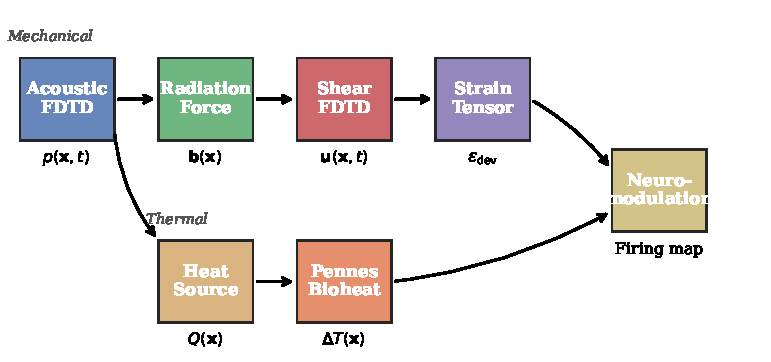
\includegraphics[width=0.92\linewidth]{fig1_pipeline.pdf}
\caption{Pipeline schematic (manuscript Fig.~1). Mechanical branch (top): acoustic FDTD $p(\mathbf{x},t)$ $\to$ radiation force $\mathbf{b}(\mathbf{x})$ $\to$ shear FDTD $\mathbf{u}(\mathbf{x},t)$ $\to$ deviatoric strain $\varepsilon_{\mathrm{dev}}$. Thermal branch (bottom): heat source $Q(\mathbf{x})$ $\to$ Pennes bioheat $\Delta T(\mathbf{x})$. Both feed the neuromodulation block, producing the per-voxel firing map. The validation report sections mirror this structure: \S\ref{sec:acoustic_inputs}--\ref{sec:acoustic_outputs} cover the acoustic-FDTD inputs and outputs (top-left), \S\ref{sec:thermal_outputs} the bioheat (bottom), \S\ref{sec:elastic_outputs} the radiation-force / shear-FDTD / strain block (top-middle), and \S\ref{sec:neural_outputs} (when present) the neuromodulation block (top-right).}
\label{fig:pipeline}
\end{figure}

\section*{Scope}
This report validates the inputs and outputs of a single Fullwave acoustic +
shear-wave simulation, organised along the pipeline branches of
Fig.~\ref{fig:pipeline}. Section~\ref{sec:acoustic_inputs} covers the
inputs to the acoustic FDTD; subsequent sections cover acoustic outputs,
thermal rise, elastic outputs (ARF / strain / membrane tension), and
the per-voxel neural firing map.

\section{Acoustic Inputs}\label{sec:acoustic_inputs}

\subsection{Parameters at a glance}\label{sec:params_compact}

\begin{table}[h!]
\centering
\scriptsize
\setlength{\tabcolsep}{4pt}
\renewcommand{\arraystretch}{1.05}
\begin{minipage}[t]{0.32\linewidth}\centering
\textbf{Grid \& timing}\\[2pt]
\begin{tabular}{lr}
\toprule
$f_0$               & 500 kHz \\
$c_0$               & 1540 m/s \\
PPW                 & 10 \\
CFL                 & 0.20 \\
$dx$                & 0.308 mm \\
$dt$                & 40.00 ns \\
Domain              & 130 $\times$ 80 $\times$ 80 mm \\
Voxels              & 422$\times$260$\times$260 \\
$n_T$               & 4221 \\
Sim time            & 168.8 $\mu$s \\
\bottomrule
\end{tabular}
\end{minipage}\hfill
\begin{minipage}[t]{0.32\linewidth}\centering
\textbf{Source spec}\\[2pt]
\begin{tabular}{lr}
\toprule
Type             & tips\_bowl \\
$R_{\text{outer}}$ & 32.0 mm \\
$R_{\text{inner}}$ & 0.0 mm \\
ROC ($F$)        & 63.0 mm \\
Elements         & 4 \\
Layers           & 3 \\
$p_0$            & 0.40 MPa \\
Cycles           & 2 \\
Drop-off         & 2.0 \\
Voxels           & 73760 \\
\bottomrule
\end{tabular}
\end{minipage}\hfill
\begin{minipage}[t]{0.32\linewidth}\centering
\textbf{Placement}\\[2pt]
\begin{tabular}{lr}
\toprule
Scalp            &  \\
Target           & ACC\_left \\
Req. $F$         & 63 mm \\
Req. $R$         & 32 mm \\
Perp residual    & 0.65 mm \\
Scalp$\to$tgt    & 40.2 mm \\
Apex$\to$tgt     & 63.0 mm \\
Sagitta          & 8.7 mm \\
EEG offset       & auto-pick (no EEG constraint) \\
$\hat n_{3D}$    & (-0.06, -0.40, -0.91) \\
\bottomrule
\end{tabular}
\end{minipage}
\caption{FDTD grid (left), bowl source spec (center), and anatomical placement (right). Placement is derived via the SyN MNI$\to$Halle warp from the requested 10-20 scalp site to the requested cortical target.}
\end{table}


\begin{figure}[H]\centering
\includegraphics[width=0.95\linewidth]{fig_inputs_placement_3d.png}
\caption{\large\textbf{ $\to$ ACC\_left: 3D placement on the Halle skull.}\\
\normalsize Top two rows: axial / sagittal / coronal slices through the bowl apex over the native-resolution (0.125\,mm) skull CT, with the brain shown against two atlas backgrounds warped to subject space --- the MNI152 T1 template (row~1) and the Harvard-Oxford cortical parcellation (row~2) --- and the bowl outline drawn in plane. Bottom row: three 3D camera angles with bowl wireframe, outer-bone surface, pial brain mesh, and target ROI. The target region (green) is the warped Harvard-Oxford label, or a 12\,mm sphere about the MNI coordinate when the target has no atlas label.}\label{fig:placement_3d}
\end{figure}


\begin{figure}[H]\centering
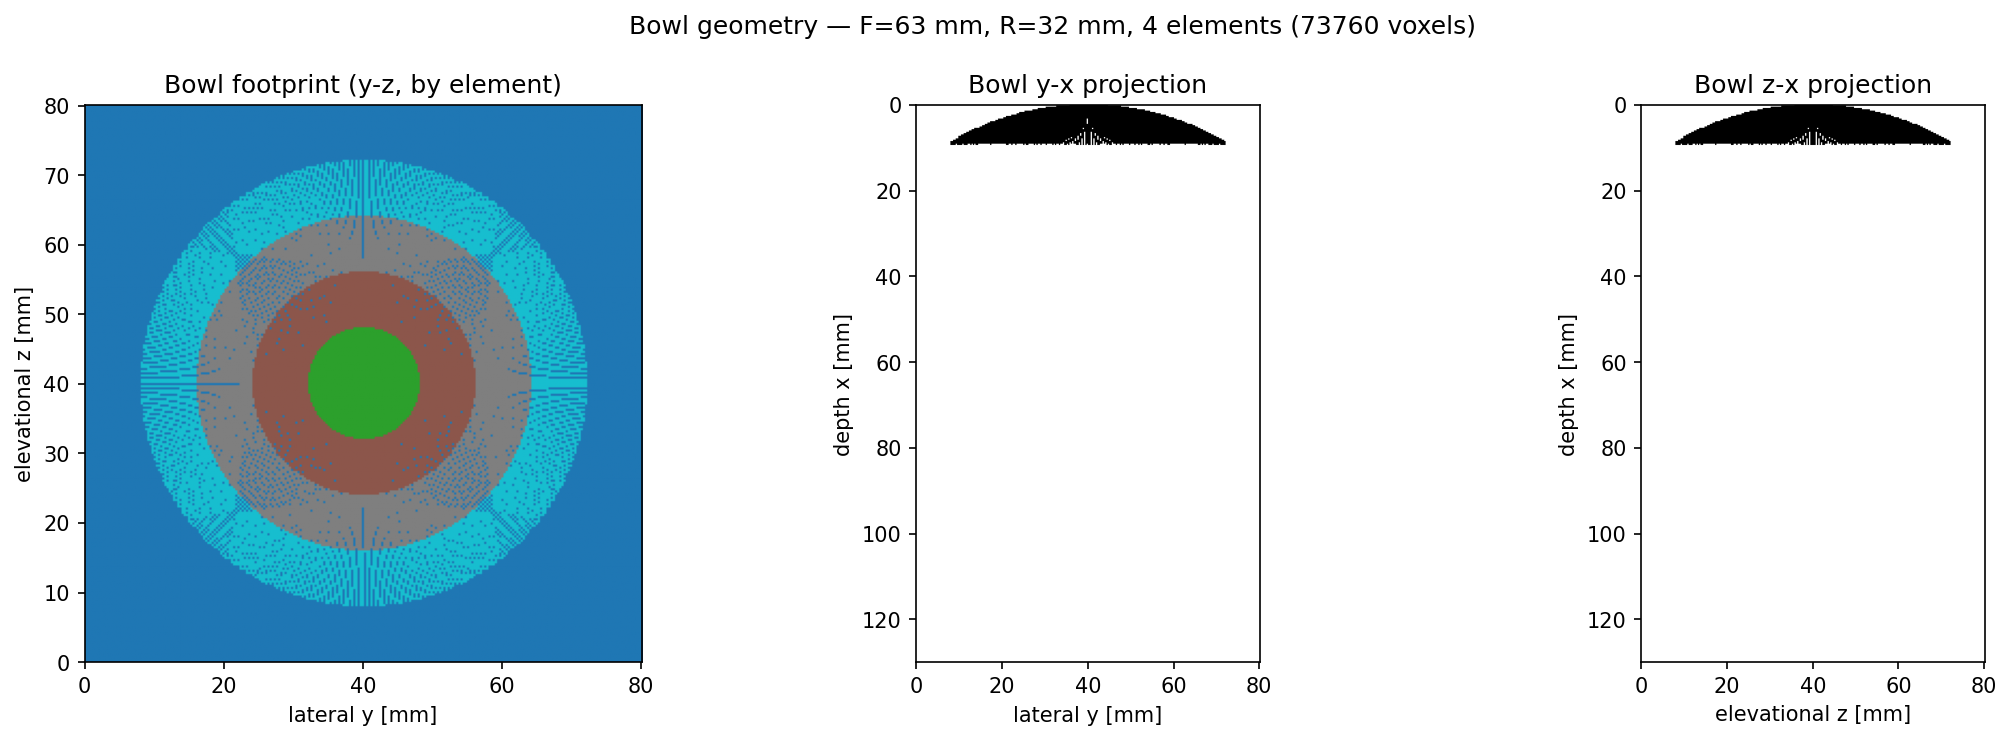
\includegraphics[width=\linewidth]{fig_inputs_bowl_geometry.png}
\caption{Bowl source mask on the FDTD slab grid: y-z aperture footprint colored by annular element (left), x-y projection (middle), x-z projection (right).}\label{fig:bowl_geom}
\end{figure}

\subsection{Acoustic medium}\label{sec:medium}
\begin{table}[h!]
\centering
\scriptsize
\setlength{\tabcolsep}{6pt}
\begin{tabular}{lr|lr}
\toprule
NRRD source        & \texttt{\textasciitilde{}/.cache/fullwave25/skull\_microCT\_zenodo/halle\_skull.nrrd} & HU thresholds        & 700 -- 1973 \\
Speed range req.   & 1540 -- 2900 m/s & Density range req.   & 1000 -- 2200 kg/m\(^3\) \\
Blur $\sigma$      & 0.00 mm & Background           & tissue \\
Built $c$ extent   & 1540 -- 2900 m/s & Built $\rho$ extent  & 1000 -- 2200 kg/m\(^3\) \\
Built $\alpha$ ext.& 0.50 -- 20.00 dB/(MHz cm) & Skull voxels         & 25366 \\
Built $\beta$ ext. & 4.80 -- 5.50 (dimensionless) & & \\
\bottomrule
\end{tabular}
\caption{Medium-builder configuration and resulting voxel-property extents on the slab grid.}
\end{table}

\begin{figure}[H]\centering
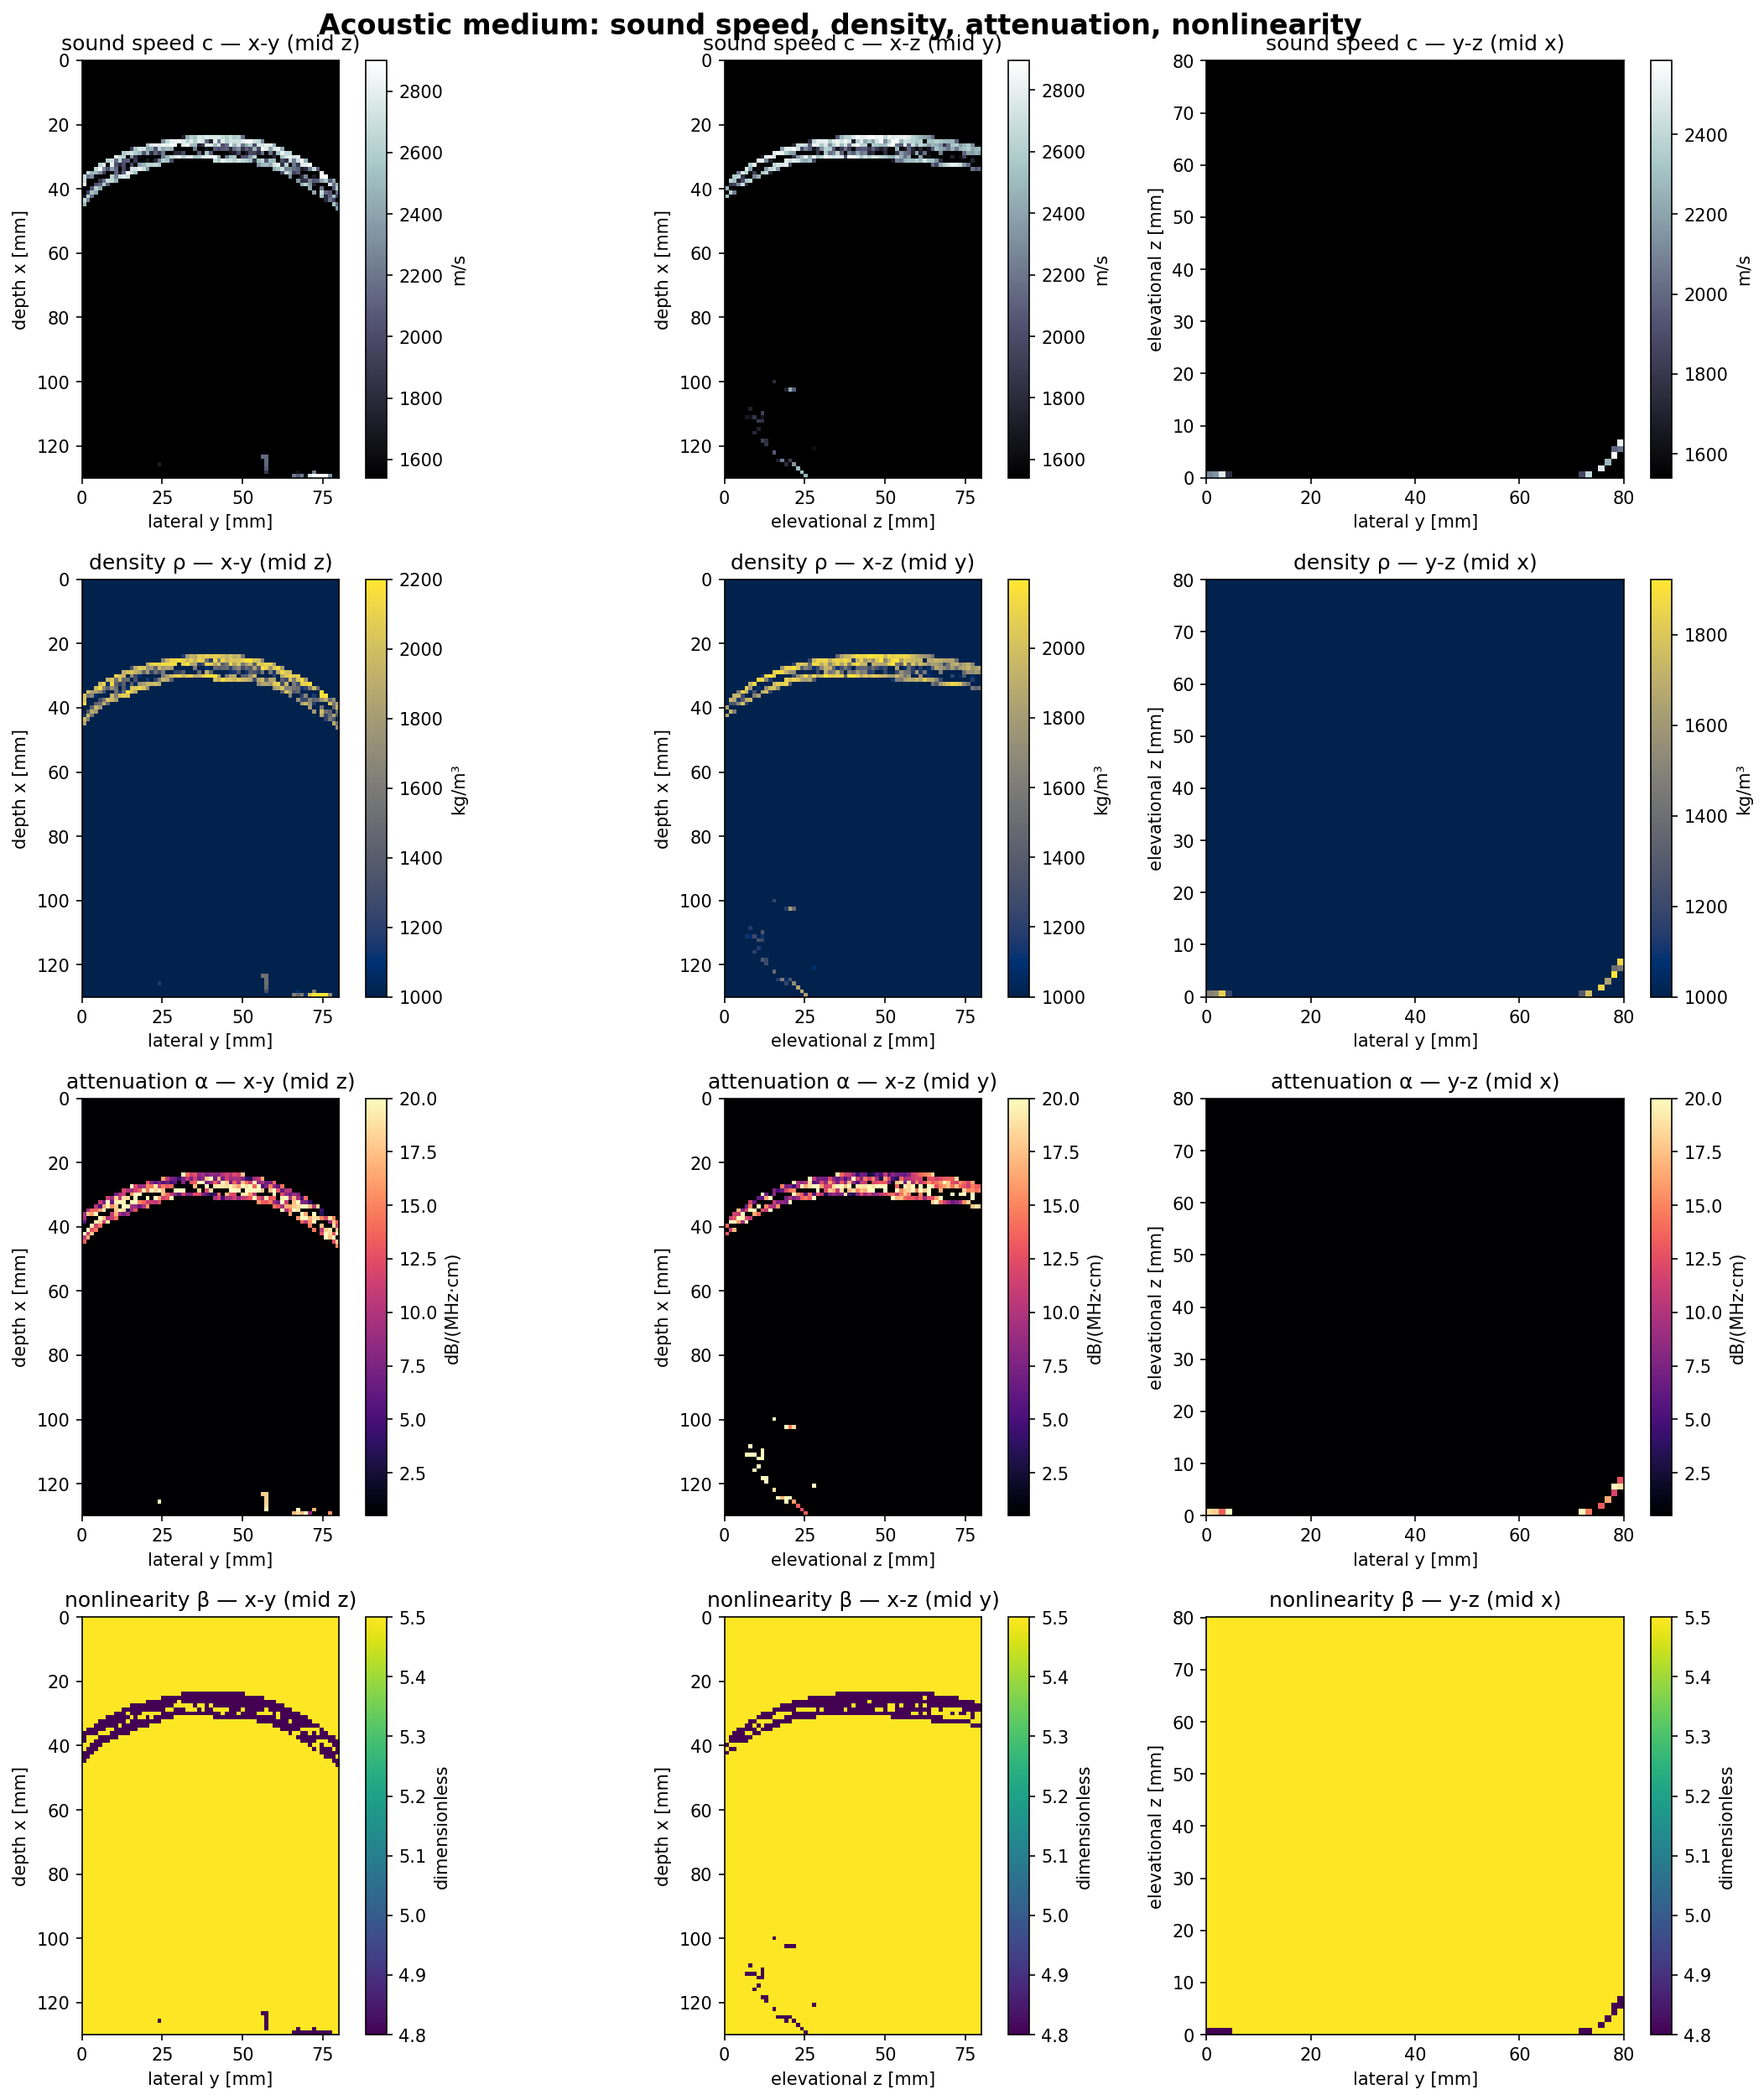
\includegraphics[width=\linewidth]{fig_inputs_medium.png}
\caption{Acoustic medium maps: sound speed $c$, density $\rho$, power-law attenuation $\alpha$, and nonlinearity coefficient $\beta$. Each row shows orthogonal mid-slices in x-y, x-z, and y-z.}\label{fig:medium}
\end{figure}

\subsection{Excitation waveform (per-pulse)}\label{sec:excitation}
\begin{figure}[H]\centering
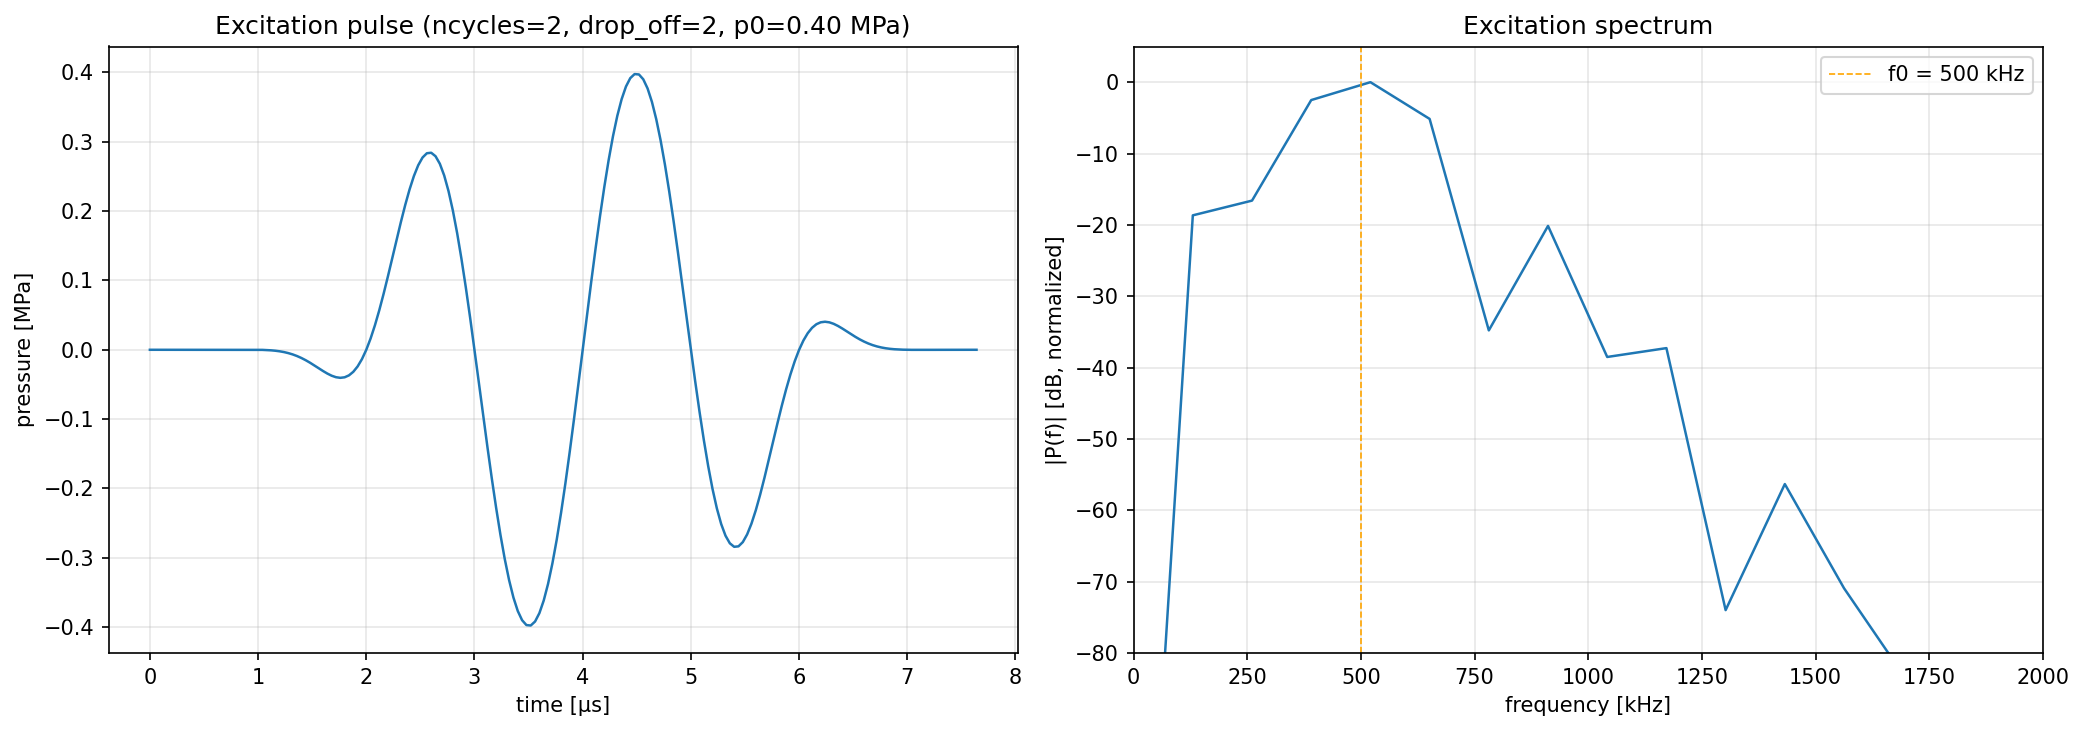
\includegraphics[width=\linewidth]{fig_inputs_excitation.png}
\caption{Per-voxel excitation pulse driving every bowl voxel (left) and its magnitude spectrum (right). All voxels fire the same pulse; geometric focusing arises from the bowl curvature.}\label{fig:excitation}
\end{figure}

\begin{table}[h!]
\centering
\scriptsize
\setlength{\tabcolsep}{6pt}
\begin{tabular}{lr|lr|lr}
\toprule
Cycles                  & 2 & Drop-off               & 2.0 & $p_0$                  & 0.40 MPa \\
$n_{\text{tic}}$        & 192   & Pulse duration         & 7.68 $\mu$s & CW correction          & 2.609 \\
Firing voxels           & 73760 & & & & \\
\bottomrule
\end{tabular}
\caption{Per-pulse excitation parameters derived from the source spec.}
\end{table}



\subsection{Neuromodulation sequence}\label{sec:sequence}

The FDTD captures the 20.0 ms
acoustic-radiation-force push window. The full session-level pulse schedule
that this push is embedded in is summarised below.


\begin{figure}[H]\centering
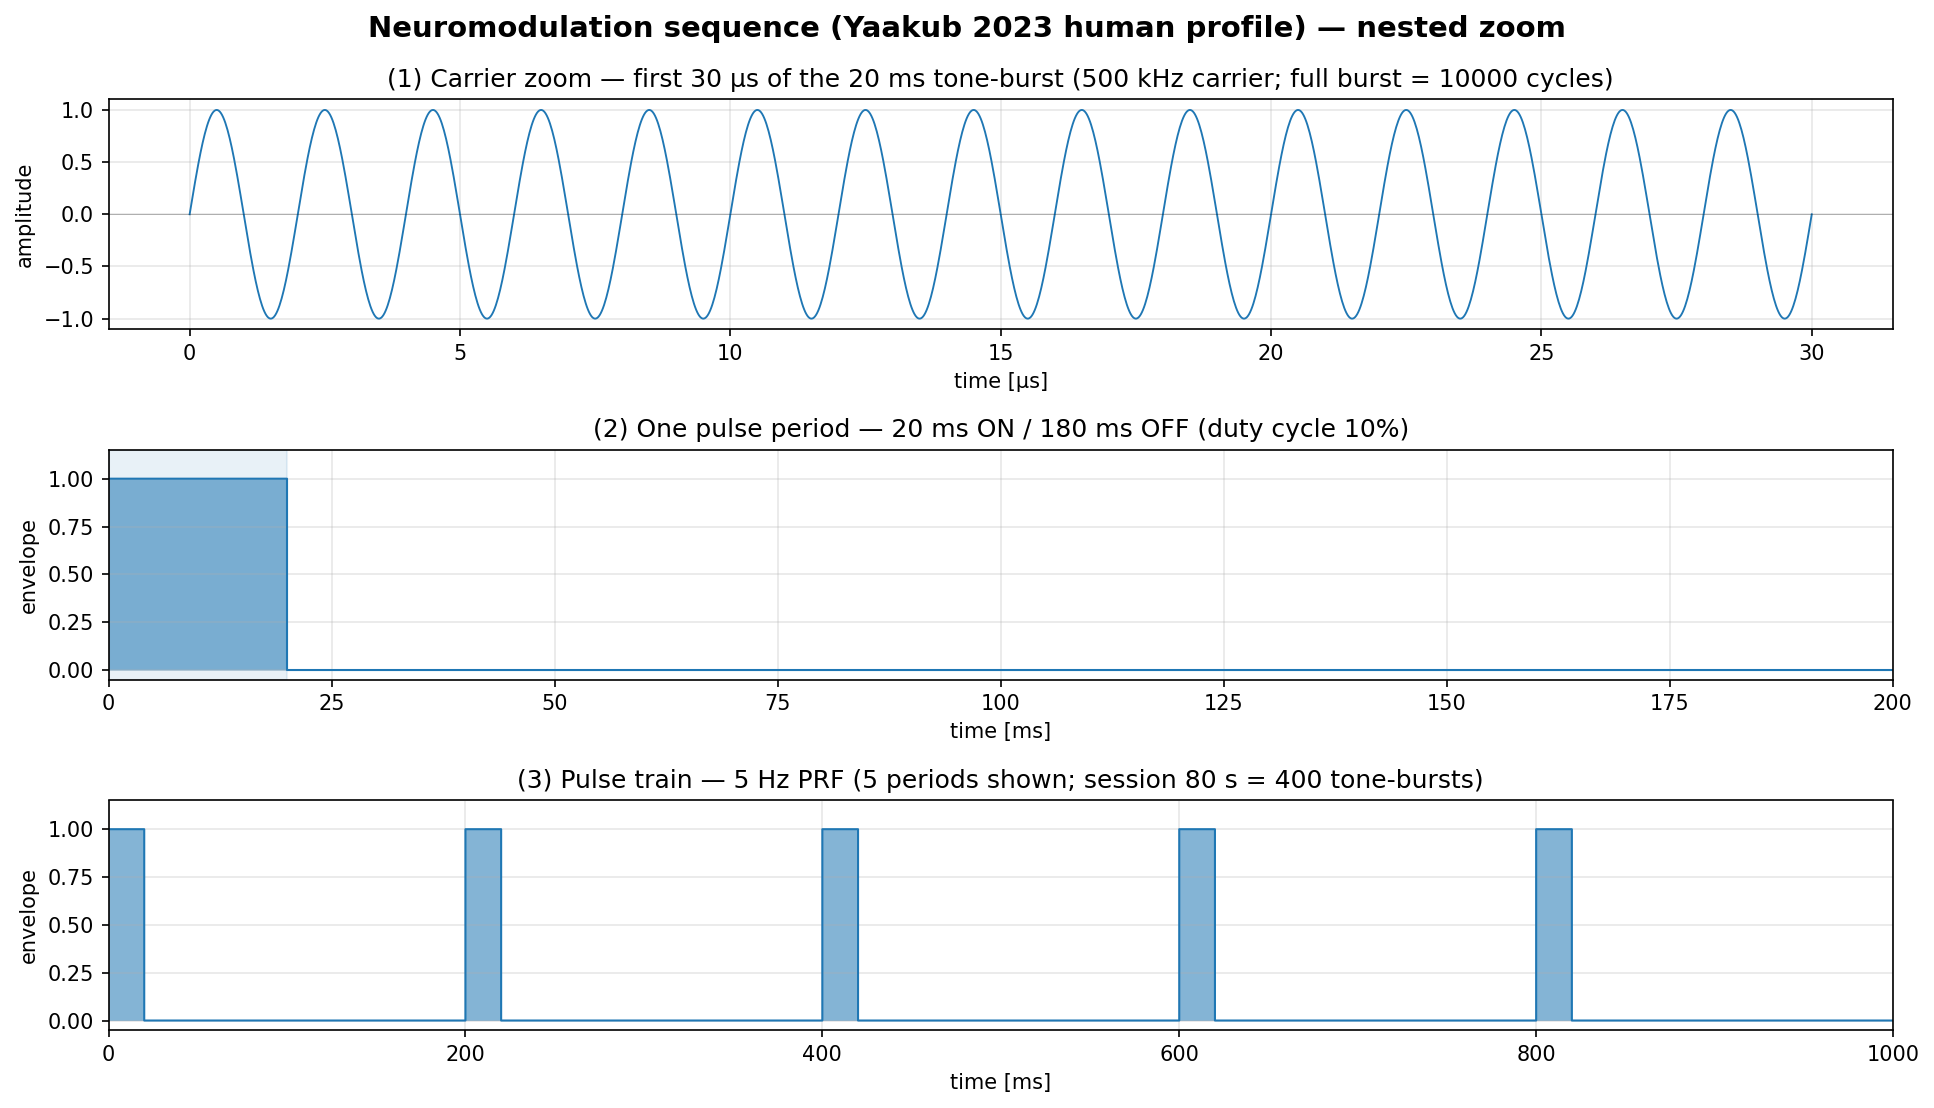
\includegraphics[width=\linewidth]{fig_inputs_sequence.png}
\caption{Yaakub 2023 human TUS protocol shown at three nested time scales: a zoom of the 500 kHz carrier within the tone-burst (top), one 200 ms pulse period showing 20 ms ON / 180 ms OFF (middle), and a 5 Hz pulse train across five periods (bottom).}\label{fig:sequence}
\end{figure}


\begin{table}[h!]
\centering
\scriptsize
\setlength{\tabcolsep}{6pt}
\begin{tabular}{lr|lr}
\toprule
Profile                         & yaakub\_human & Envelope                & rectangular CW tone-burst (no nested sub-bursts) \\
Carrier $f_0$                   & 500 kHz & Tone-burst duration     & 20 ms \\
PRF                             & 5.0 Hz & Pulse period            & 200 ms \\
Duty cycle                      & 10 \% & ISI (off-time)          & 180 ms \\
Session duration                & 80 s & Pulses per session      & 400 \\
ARF push window (FDTD)          & 20.0 ms & Target $I_{\text{SPPA}}$ & 30 W/cm\(^2\) \\
\bottomrule
\end{tabular}
\caption{Session-level TUS protocol (Yaakub 2023 human profile). The FDTD solves one tone-burst's ARF window; the table shows how that push is repeated in vivo.}
\end{table}




\section{Acoustic Outputs}\label{sec:acoustic_outputs}


\subsection{Pulse normalization and gating}\label{sec:pulse_norm}

The saved propagation map records a tone burst that is silent for most
of the saved window.  Recovering a continuous-wave-equivalent intensity
field requires two multiplicative corrections applied to the time-mean
of $p^2$: the silence correction lifts the full-window mean to the
active-pulse-window mean, and the cw correction (Gaussian-envelope
peak vs.\ sinusoidal RMS) lifts further to a continuous-wave reference.

\begin{table}[h!]
\centering
\scriptsize
\setlength{\tabcolsep}{6pt}
\begin{tabular}{lr|lr}
\toprule
$n_t$ saved (snapshots)            & 603                          & $n_{\mathrm{tic}}$ (source steps, full grid) & 192 \\
Sampling modulus time $\mathrm{smt}$ & 7          & Source steps saved $n_{\mathrm{tic}}/\mathrm{smt}$ & 27 \\
Silence correction $n_t / n_{\mathrm{src}}$ & 22.33 & CW correction (burst envelope) & 2.609 \\
\multicolumn{3}{r}{Pulse normalization (silence $\times$ cw)} & 58.27 \\
\bottomrule
\end{tabular}
\caption{Pulse-gating constants used to convert the saved $\langle p^2 \rangle$ field into a continuous-wave-equivalent intensity. The silence correction is the ratio of total saved snapshots to the number of active source steps (= $n_{\mathrm{tic}} / \mathrm{smt}$); the cw correction lifts the Gaussian-burst peak to a sinusoidal-RMS reference; their product is multiplied into $\langle p^2 \rangle$ before computing the intensity field rendered in Figs.~\ref{fig:acoustic_intensity}.}
\label{tab:pulse_norm}
\end{table}

\paragraph{Scaling the short-pulse output to a long-pulse exposure.}
The Fullwave run simulates a short Gaussian-windowed tone-burst of $n_{\mathrm{src}}$ active source steps embedded in $n_t$ saved snapshots, after which the source is silent and the field rings down.  The saved $\langle p^2 \rangle_{xyz}(t)$ has two regimes: an \emph{active-pulse window} where the spatial mean tracks the Gaussian burst envelope, and a \emph{silent ring-down} window where stored energy decays through the absorbing boundaries.  The two pulse-normalization constants in Table~\ref{tab:pulse_norm} convert this short-pulse output into the continuous-wave-equivalent intensity that an arbitrarily long real-world pulse would produce.

The \emph{silence correction} $n_t / n_{\mathrm{src}}$ is the duty-factor inverse: averaging $\langle p^2 \rangle$ over the full $n_t$-step window dilutes its value by the fraction of the window for which the source is actually emitting, so multiplying by $n_t / n_{\mathrm{src}}$ recovers the time-averaged $\langle p^2 \rangle$ of a CW source.  The \emph{cw correction} (typically $\approx 0.5$ for a half-sinusoid burst envelope, with the exact value tabulated) is the ratio of the burst's mean-square to a unit-amplitude CW sinusoid's mean-square; dividing $\langle p^2 \rangle$ by it lifts the Gaussian-burst peak to a sinusoidal-RMS reference.  Their product (silence $\times$ cw, also tabulated as ``Pulse normalization'') is the single multiplicative factor applied to the saved $\langle p^2 \rangle$ before the intensity field shown in Figs.~\ref{fig:acoustic_intensity} is computed.

Energy conservation then gives the relationship between the short and long pulses directly: a CW source delivering the same per-cycle PNP as the simulated burst deposits energy at a rate $n_t / n_{\mathrm{src}}$ times higher (the silence factor has the dimensions of a duty inverse), so total energy and time-averaged intensity scale by the same constant.  Peak quantities (PNP, PPP, MI) are unaffected by the correction; cumulative quantities ($I_{\mathrm{SPTA}}$, thermal index, $\Delta T$) all scale linearly with the pulse-normalization factor and therefore with simulated burst length once the geometry of the field has converged.

\subsection{Exposure metrics}\label{sec:exposure_metrics}

The metrics below are computed directly from the saved Fullwave acoustic
output (per-voxel pressure-time history, particle velocity, and
radiation-force density) on the downsampled validation grid, after the
pulse-normalization correction in Table~\ref{tab:pulse_norm}.  The
$\Delta T$ and strain-derived rows are produced by the bioheat and
shear-wave sub-pipelines and are reported in their own sections.

\begin{table}[h!]
\centering
\scriptsize
\setlength{\tabcolsep}{6pt}
\renewcommand{\arraystretch}{1.05}


\begin{tabular}{l r  l}
\toprule
\textbf{Quantity} & \textbf{Transcranial}  & \textbf{Unit} \\
\midrule
PNP                                  & 0.485        & MPa \\
PPP                                  & 0.500        & MPa \\
Mechanical Index                     & 0.69             & - \\
Thermal Index (soft tissue)          & 4.147        & - \\
Thermal Index (cranial)              & 21.771     & - \\
$I_{\mathrm{SPPA}}$                  & 8.12    & W/cm$^2$ \\
$I_{\mathrm{SPTA}}$                  & 8.117    & W/cm$^2$ \\
ARF density                          & 323.02   & N/m$^3$ \\
$-6$\,dB volume                      & 161 & mm$^3$ \\
FWHM lateral ($y$)                   & 3.70      & mm \\
FWHM elevation ($z$)                 & 3.70      & mm \\
FWHM axial ($x$)                     & 22.18      & mm \\
$\langle I \rangle$ in $-6$\,dB vol  & 5.29   & W/cm$^2$ \\
Peak particle velocity               & 1.186e-08 & m/s \\
ARF impulse / pulse                  & 6.460e+00 & Pa$\cdot$s \\
\bottomrule
\end{tabular}
\caption{Acoustic exposure metrics from the FDTD output.  ISPTA uses the within-burst duty cycle of 1.00; pulse duration 20000.00 $\mu$s.  Strain-derived and bioheat-derived rows ($\Delta T$, peak strain, peak strain rate, peak strain gradient) are reported in subsequent sections.}
\label{tab:acoustic_outputs}
\end{table}

\subsection{Pressure snapshots — early / focal / post-focal}\label{sec:pressure_snapshots}
\begin{figure}[H]\centering
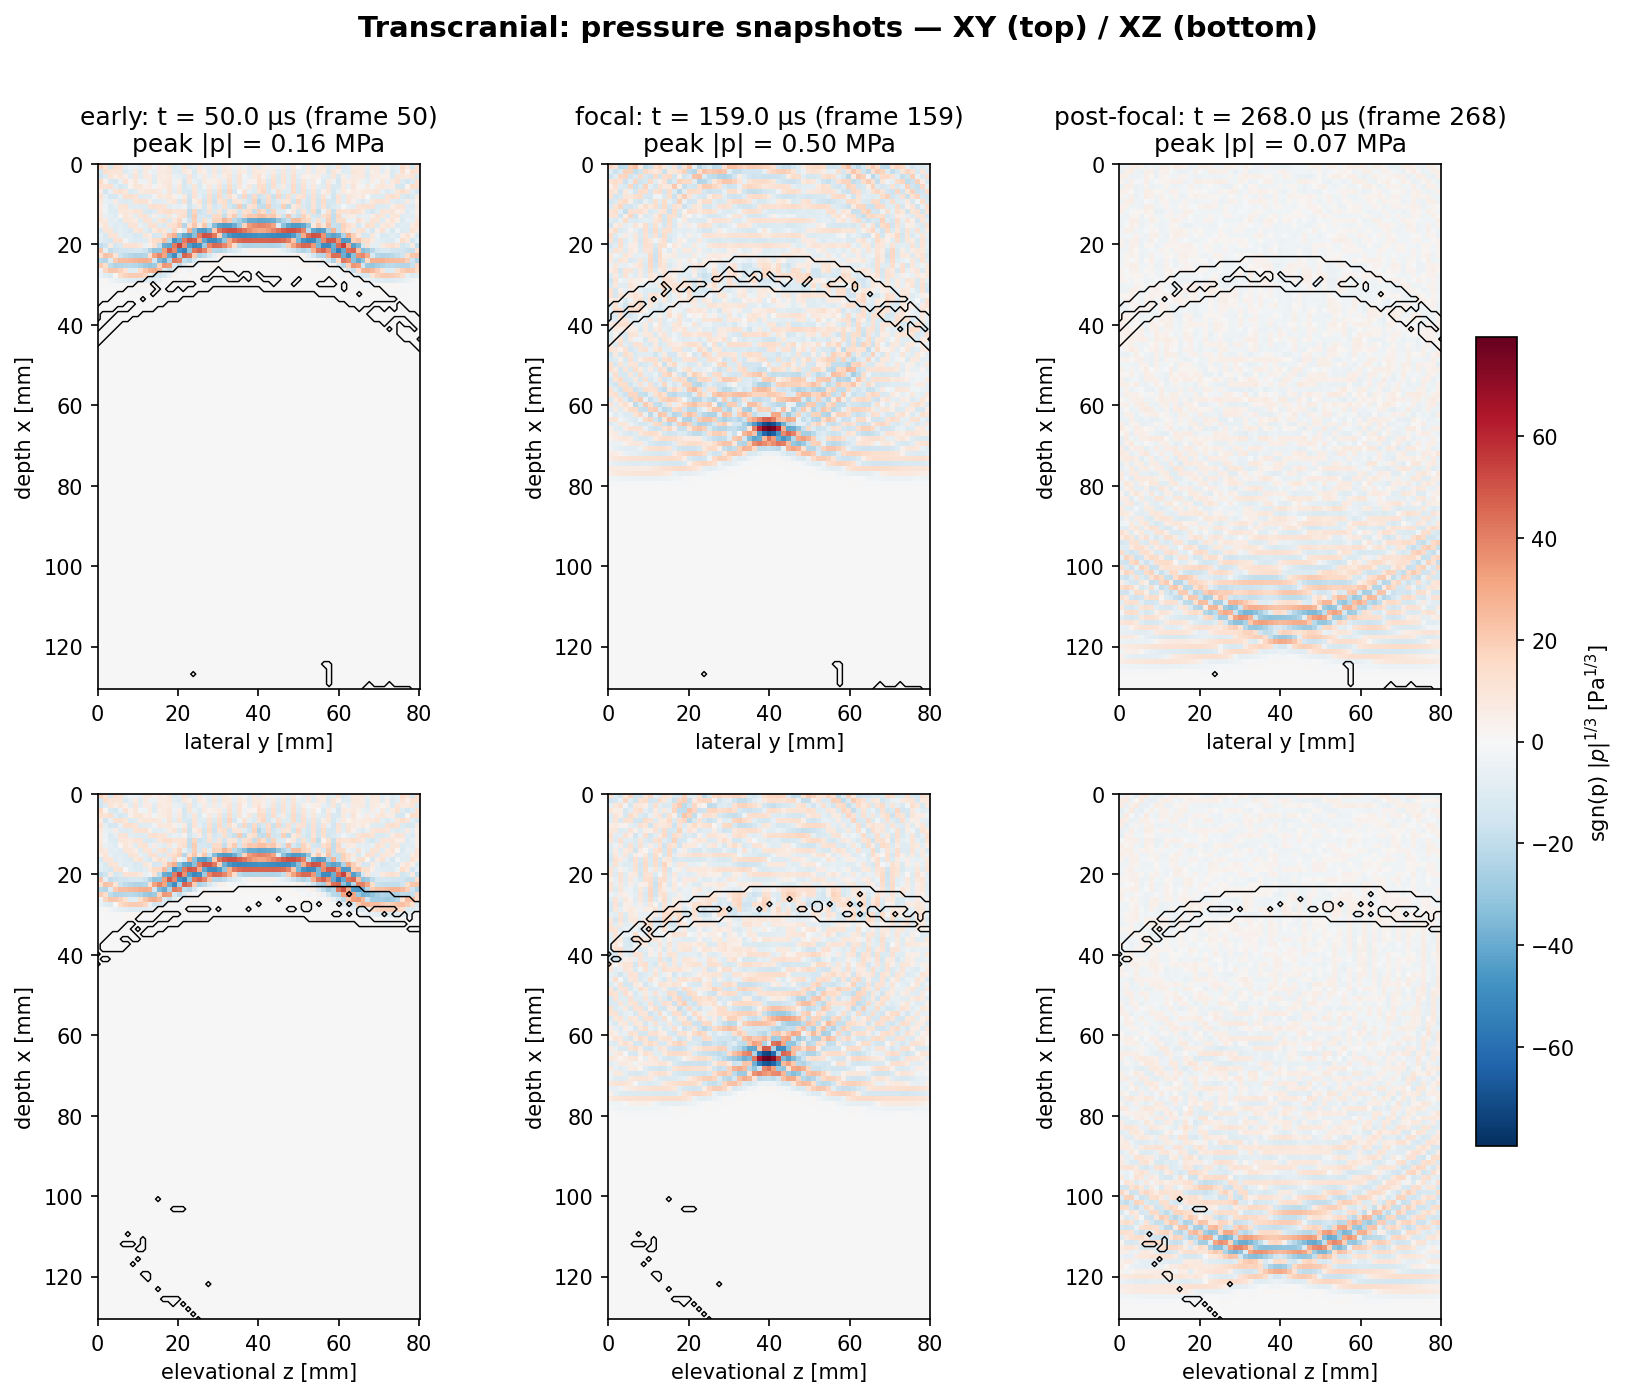
\includegraphics[width=\linewidth]{acoustic_pressure_snapshots.png}
\caption{Acoustic pressure snapshots at three timepoints: early (wave entering the domain), focal (global peak $|p|$), and post-focal (wave past the geometric focus). Top row: XY mid-z slices; bottom row: XZ mid-y slices. Colorscale is the sign-preserving cube-root compression $\mathrm{sgn}(p)\,|p|^{1/3}$ to make low-amplitude propagating wavefronts visible alongside the focal peak. Black contour outlines the skull mask ($c > 1600$\,m/s). Frame indices, timepoints, and per-frame peak $|p|$ in MPa are annotated above each panel.\\
{\scriptsize Frames: early $t=50.0$ µs (peak $|p|=0.16$ MPa) | focal $t=159.0$ µs (peak $|p|=0.50$ MPa) | post $t=268.0$ µs (peak $|p|=0.07$ MPa). Global peak $|p|=0.50$ MPa.}}\label{fig:pressure_snapshots}
\end{figure}

\subsection{Focal intensity — slices and 3D iso-surfaces}\label{sec:intensity}
\begin{figure}[H]\centering
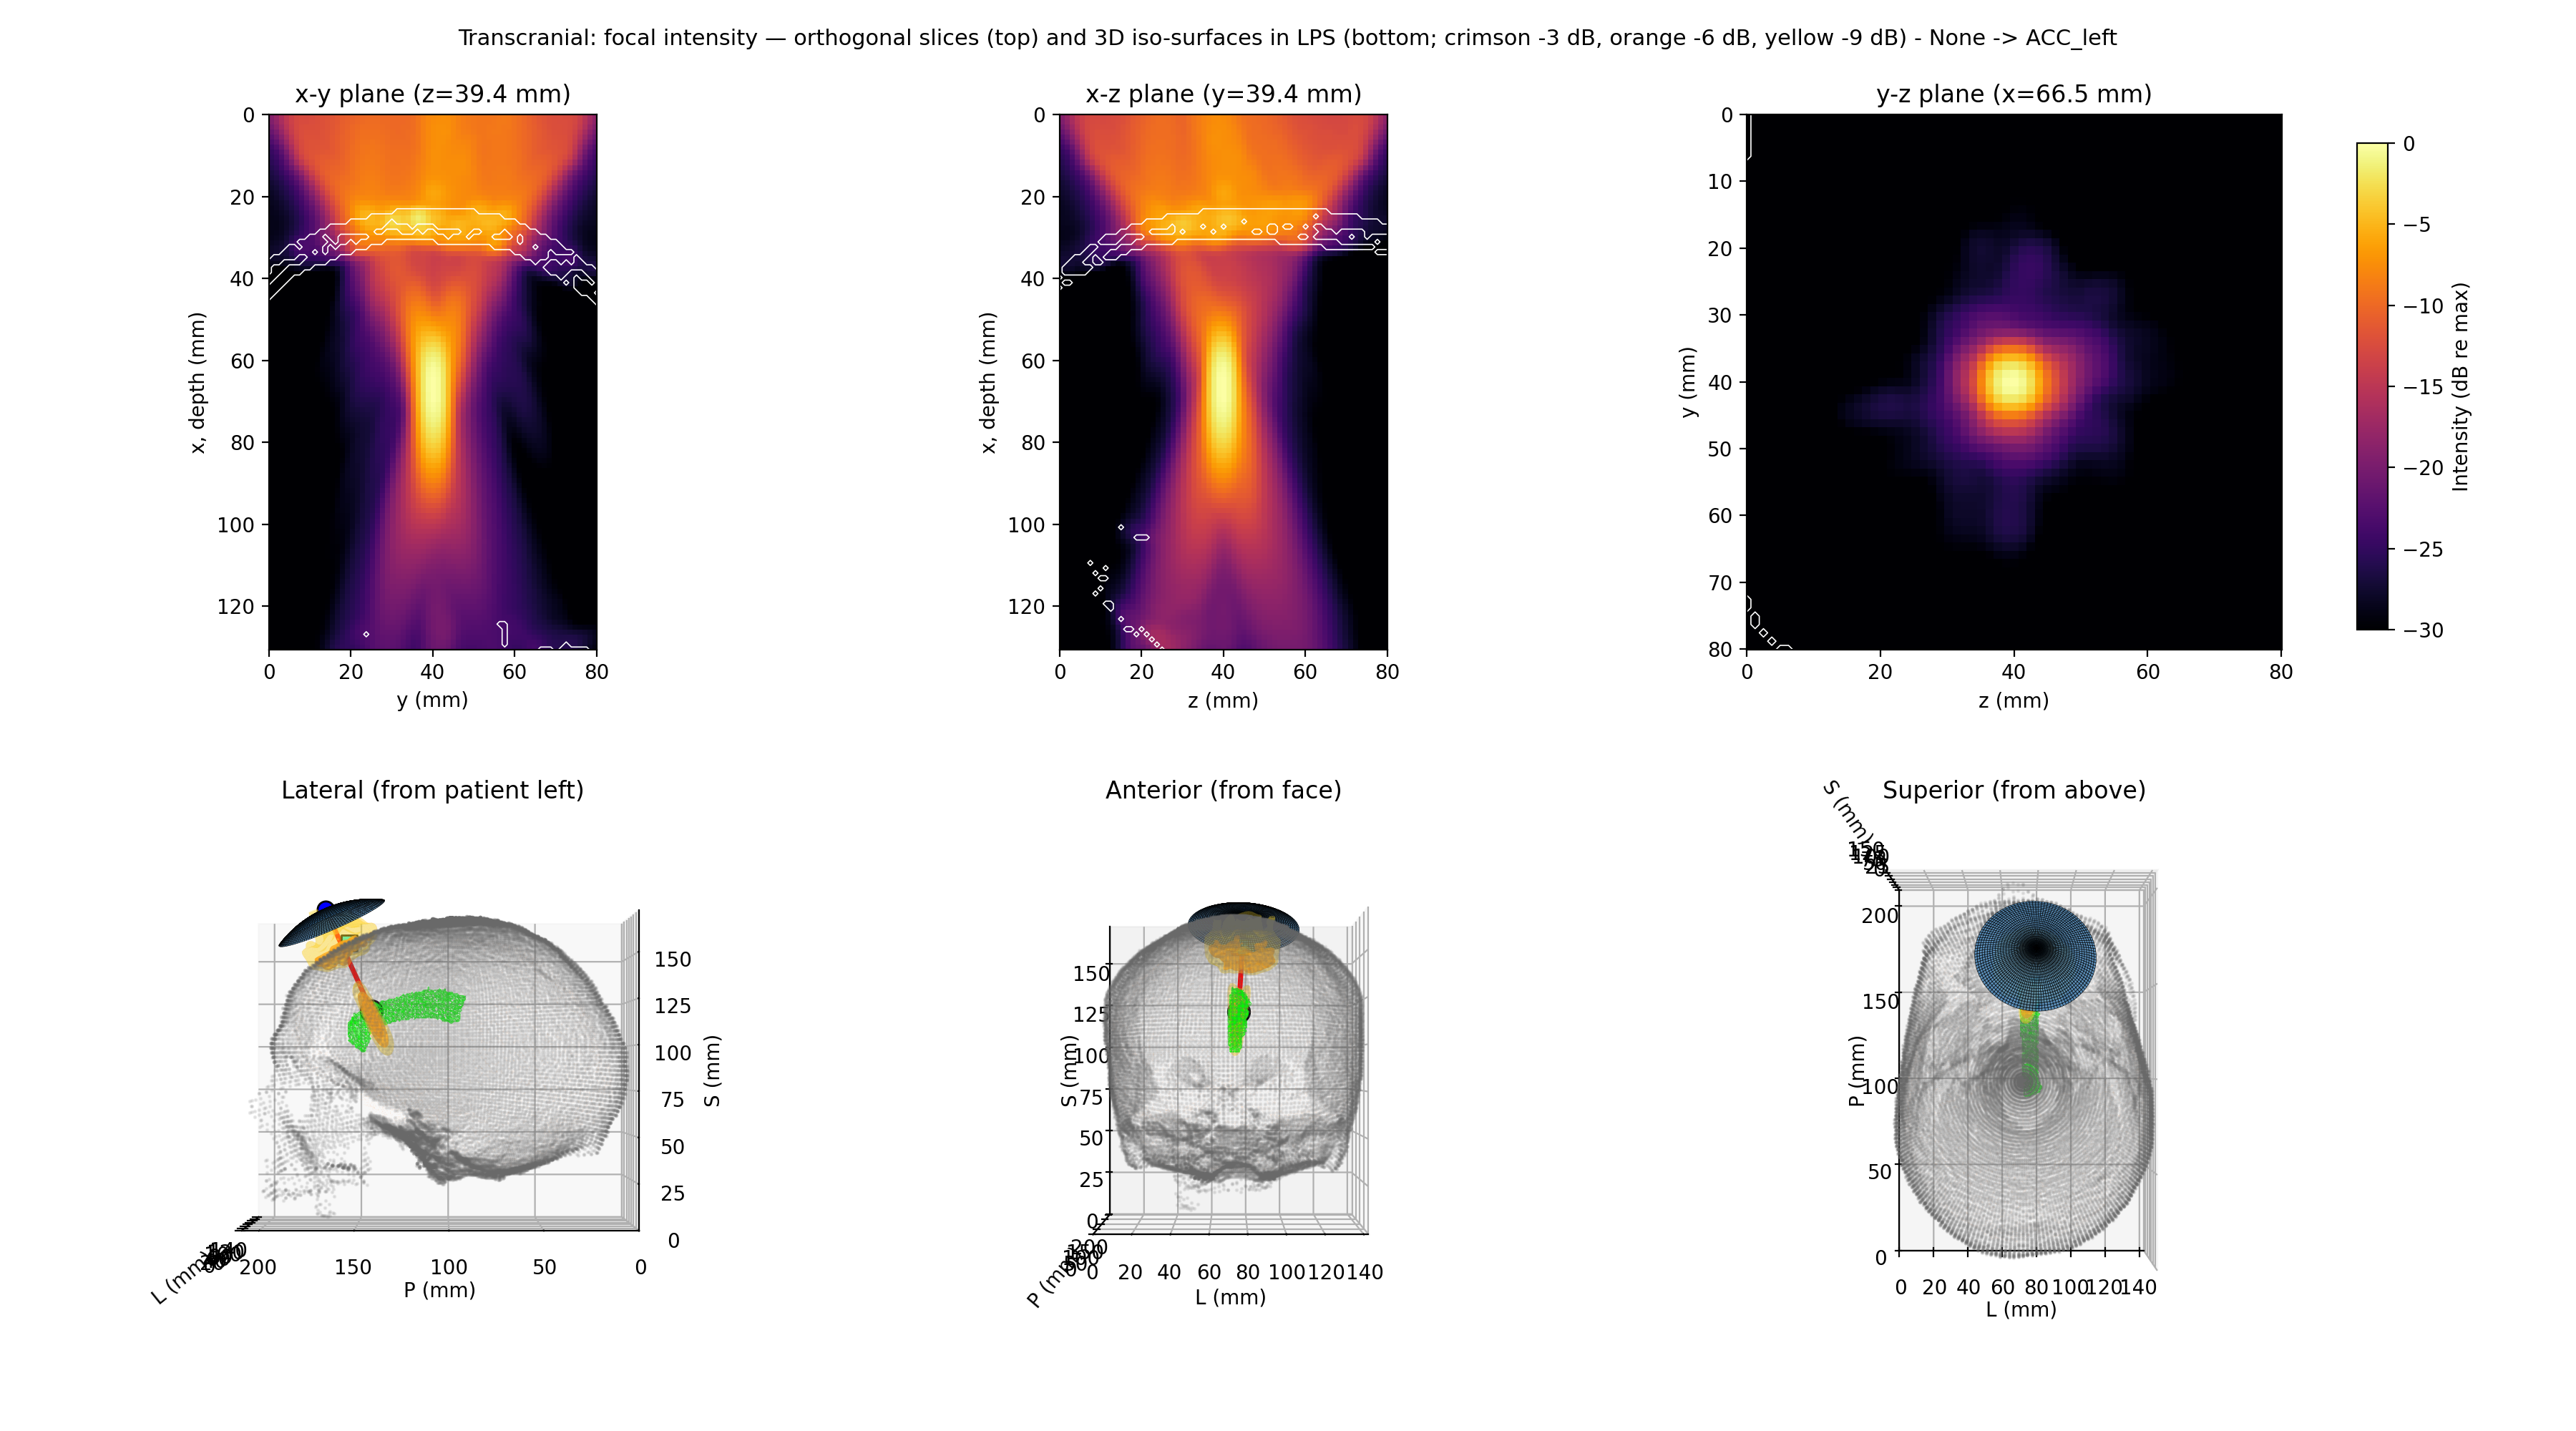
\includegraphics[width=\linewidth]{acoustic_intensity_combined.png}
\caption{Top: orthogonal slices of intensity through the focal voxel in dB re max, with the skull mask ($c > 1700$\,m/s) contoured in white. Bottom: same focal lobe rendered in LPS coordinates with the skull point cloud, pial brain mesh, target ROI (lime), and bowl wireframe (steelblue), viewed from three camera angles. Nested iso-surfaces: crimson $-3$ dB, orange $-6$ dB, yellow $-9$ dB.}\label{fig:acoustic_intensity}
\end{figure}







\section{Thermal Outputs}\label{sec:thermal_outputs}


\subsection{Thermal-rise metrics}\label{sec:thermal_metrics}

The Pennes bioheat equation is solved on the same downsampled validation
grid used for Section~\ref{sec:acoustic_outputs}, driven by the heat
source $Q = 2 \alpha I$ derived from the unwrapped propagation map and
lifted to the continuous-wave reference via the same pulse normalisation
(Table~\ref{tab:pulse_norm}).  The simulation runs the full theta-burst
schedule from Section~\ref{sec:sequence}: each acoustic ON segment lasts
20~ms with an in-burst duty cycle
of 1.00, repeated every
200~ms for
400 groups (total 80.0~s).
The bioheat time step is $dt_{\mathrm{heat}} = 1.50e+00$~s.

\begin{table}[h!]
\centering
\scriptsize
\setlength{\tabcolsep}{6pt}
\renewcommand{\arraystretch}{1.05}
\begin{tabular}{lrl}
\toprule
\textbf{Quantity} & \textbf{Transcranial} & \textbf{Unit} \\
\midrule
Skull absorption fraction $f_{\mathrm{abs}}^{\mathrm{skull}}$ (Pinton 2012) & 0.30 & --- \\
\midrule
Peak $\Delta T$ at session end             & 0.9242 & K \\
Peak $\Delta T$ over the session           & 0.9364 & K \\
Brain-tissue peak $\Delta T$ (final)       & 0.7351 & K \\
Skull peak $\Delta T$ (final)              & 0.9242 & K \\
$\Delta T$ per single-burst pulse (no diffusion) & 0.0222 & K \\
CEM43 thermal dose (peak voxel)            & 8.172e-04 & min \\
\bottomrule
\end{tabular}
\caption{Thermal-rise metrics from the bioheat solve over the session-level theta-burst schedule.  Heat source $Q = 2\alpha I$ with the Pinton 2012 skull-absorption fraction $f_{\mathrm{abs}}^{\mathrm{skull}} = 0.30$ applied to skull voxels only ($c > 1600$\,m/s); soft tissue uses the full $\alpha$. The CEM43 dose is computed at the spatial-peak voxel by Sapareto--Dewey integration over the captured frame series. The single-burst $\Delta T$ row is the conduction-free upper bound $Q\cdot t_{\mathrm{on}}/(\rho c)$ at the peak voxel and is included for sanity checking.}
\label{tab:thermal_outputs}
\end{table}

\subsection{Thermal-rise time history}\label{sec:thermal_history}
\begin{figure}[H]\centering
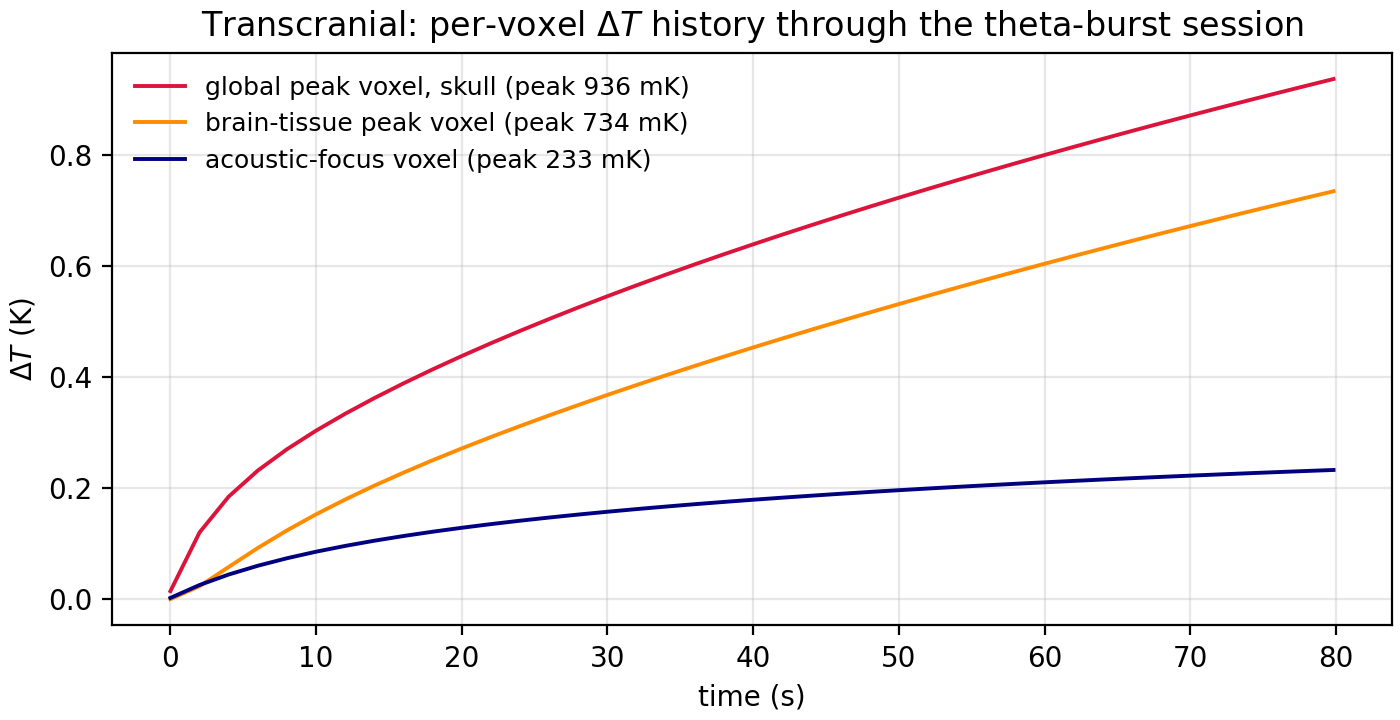
\includegraphics[width=\linewidth]{thermal_time_history.png}
\caption{Spatial-peak $\Delta T$ over the session (left), and per-frame $\Delta T$ traces (right) at two voxels: the global hot voxel (crimson, typically at the skull where attenuation is highest) and the acoustic-focus voxel inside brain tissue (navy, the brain voxel with the largest time-averaged $\langle p^2 \rangle$).  Both peak values are reported in the legend.}\label{fig:thermal_history}
\end{figure}

\subsection{Three-plane thermal-rise views}\label{sec:thermal_ortho}
\begin{figure}[H]\centering
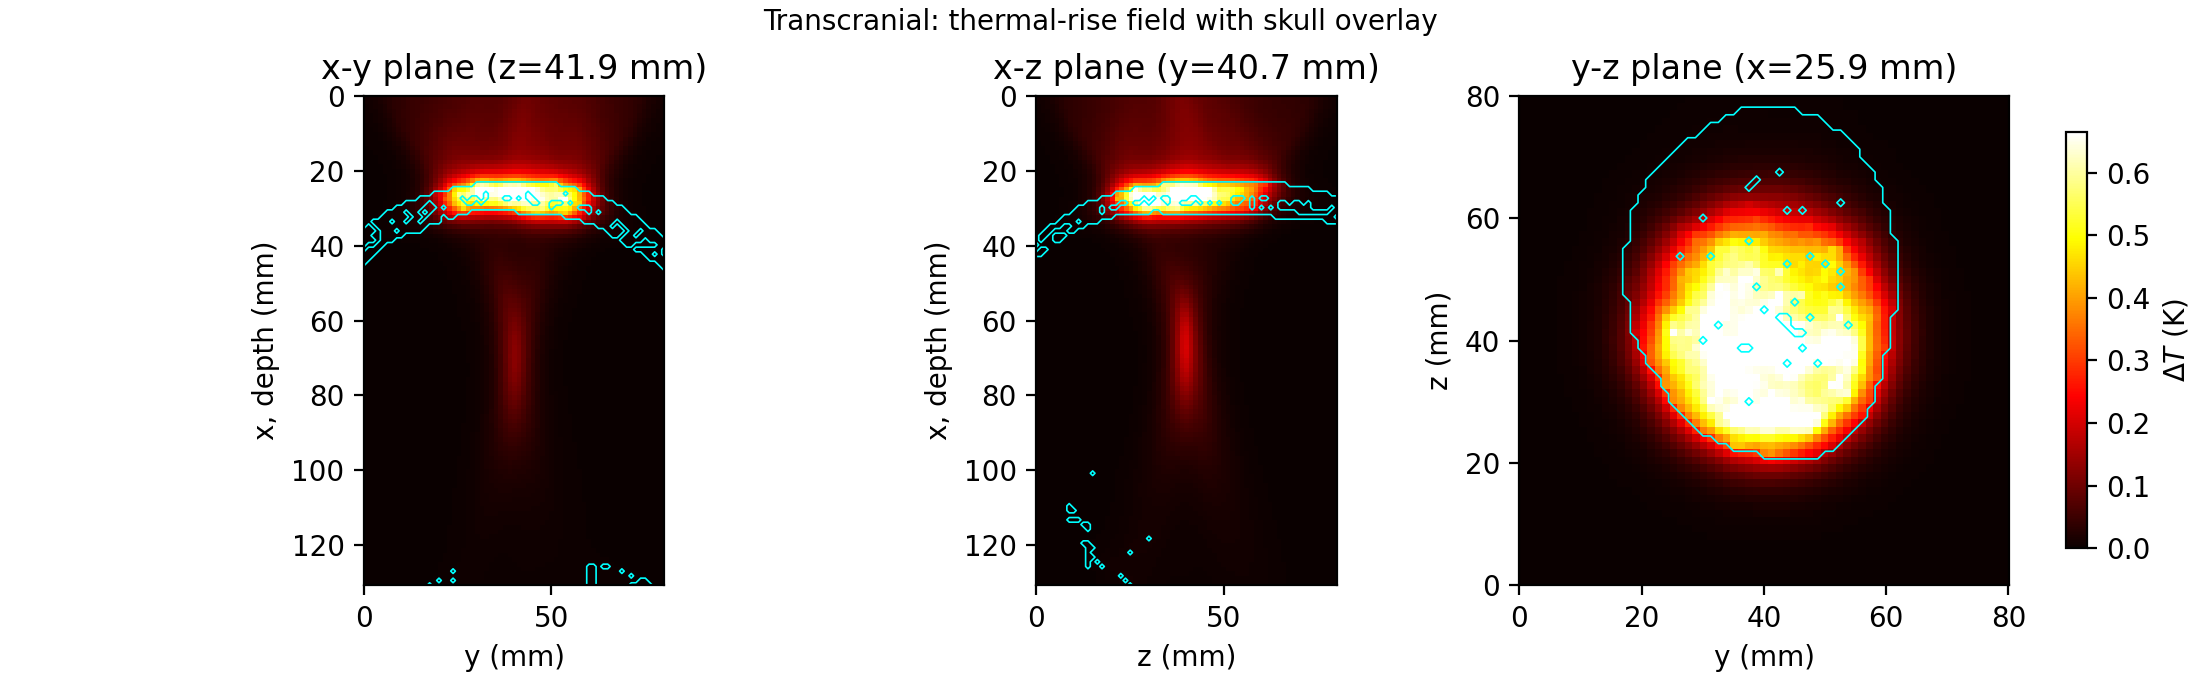
\includegraphics[width=\linewidth]{thermal_ortho_dT.png}
\caption{Orthogonal slices of $\Delta T$ at session end through the peak-temperature voxel. Depth ($x$) is on the vertical axis with 0 at the top (radiology convention); cyan contour shows the skull mask ($c > 1600$\,m/s).}\label{fig:thermal_ortho}
\end{figure}

\subsection{Three-dimensional thermal-rise rendering}\label{sec:thermal_3d}
\begin{figure}[H]\centering
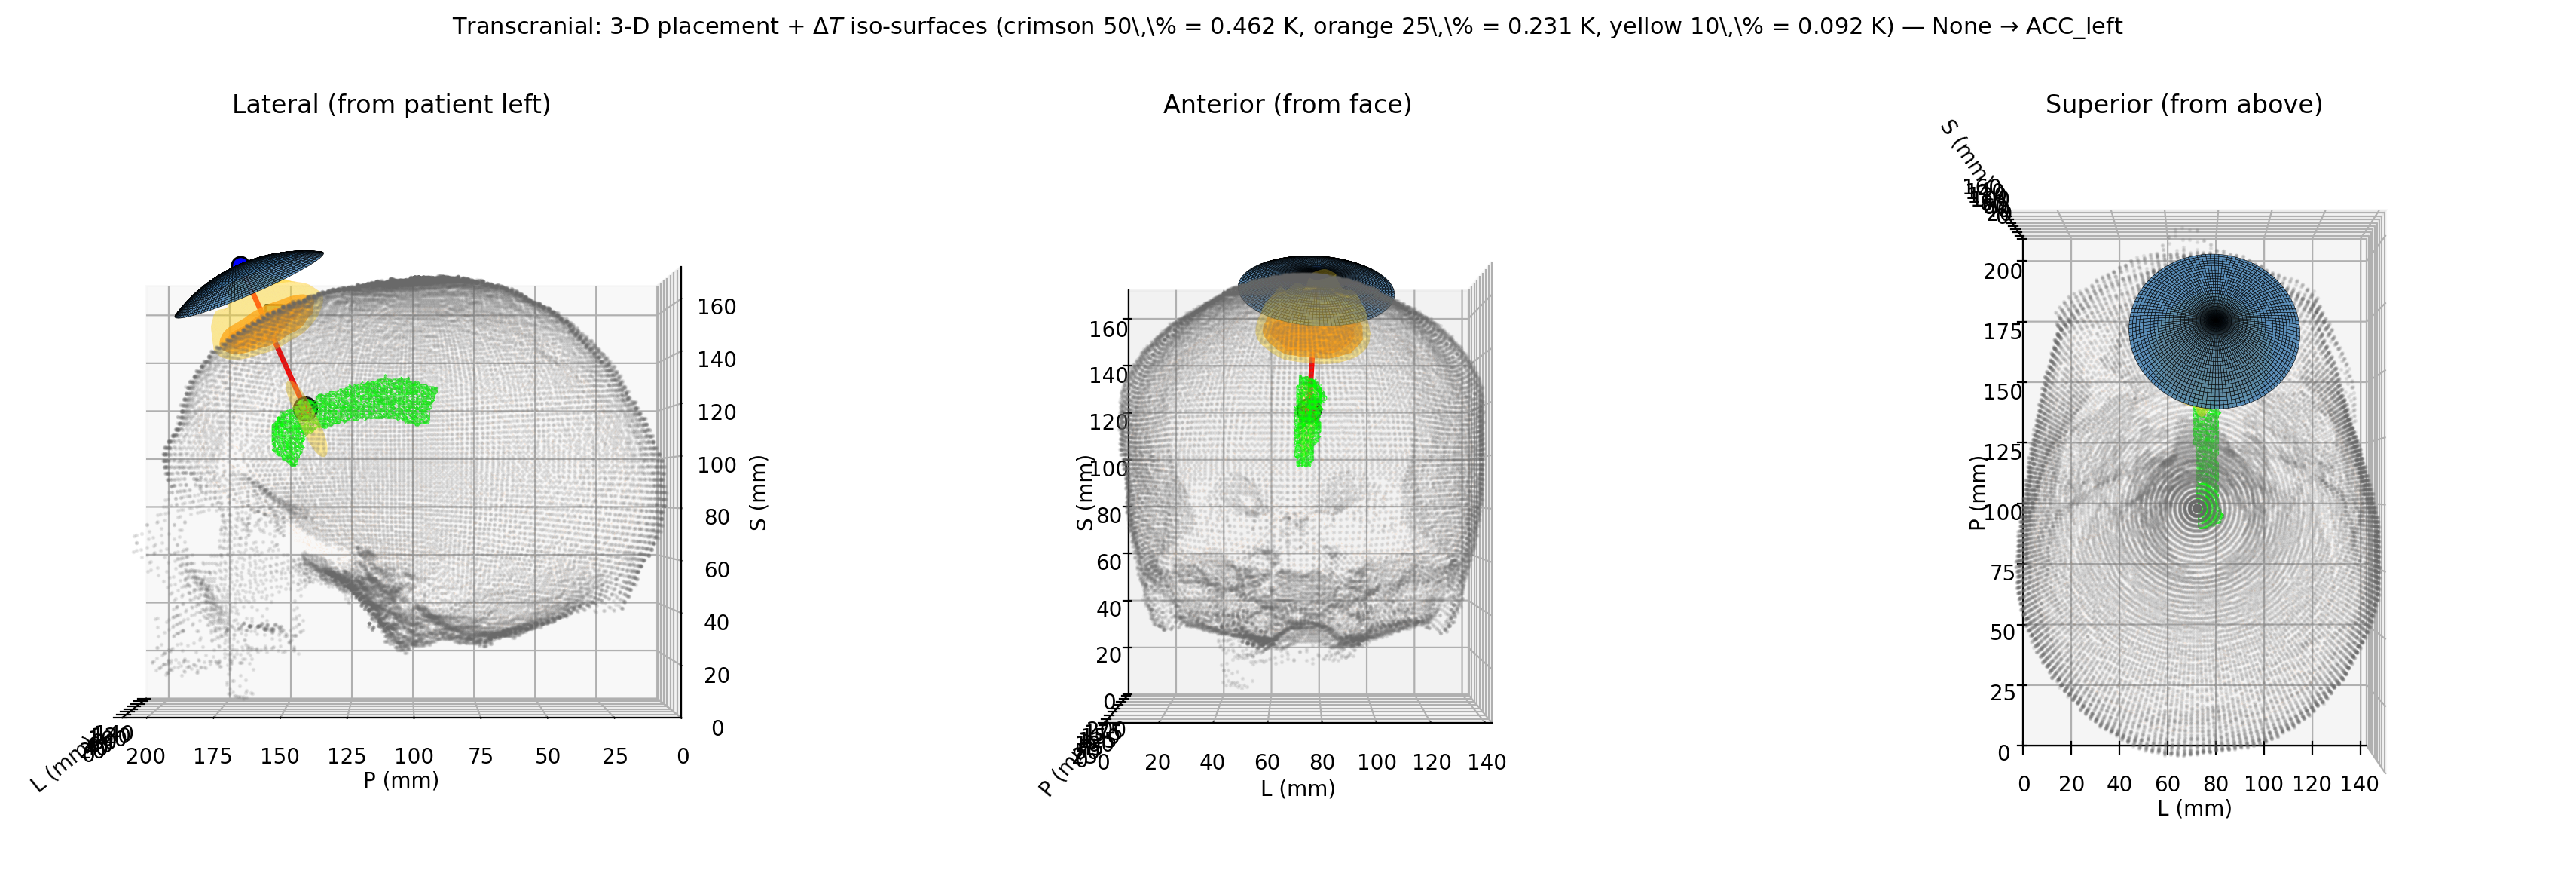
\includegraphics[width=\linewidth]{thermal_3d_dT.png}
\caption{Three-camera 3-D rendering of the $\Delta T$ field, patterned on Fig.~\ref{fig:acoustic_intensity}: full skull point cloud (grey), pial brain mesh (translucent tan), target ROI (lime), bowl wireframe (steelblue), beam axis (red line), and apex (blue) / scalp contact (cyan square) / target (lime) / focus (red star) markers, with the $\Delta T$ iso-surfaces overlaid (crimson 50\,\%, orange 25\,\%, yellow 10\,\% of peak).  Three views: lateral, anterior, superior.}\label{fig:thermal_3d}
\end{figure}







\section{Shear-Wave Displacement}\label{sec:displacement_outputs}


The transient shear-wave response to a single Yaakub tone-burst is
solved on the same downsampled validation grid as
Section~\ref{sec:acoustic_outputs} using a staggered-grid Kelvin-Voigt
elastodynamic FDTD.  The body force $\mathbf{F}_{\mathrm{ARF}}$ is
gated by a rectangular envelope (ON for 20\,ms
out of a 200\,ms PRF period); during the OFF
window the displacement relaxes under the visco-elastic body alone.
The trace at the peak ARF voxel and a sequence of $|u_x|$ snapshots
through that voxel summarise the transient.

\begin{table}[h!]\centering\small
\begin{tabular}{lr}
\hline
Peak $|u_x|$ (trace voxel)              & 0.356\,$\mu$m \\
Time to peak                            & 20.0\,ms \\
$|u_x|$ at end of ON window             & 0.355\,$\mu$m \\
Visco-elastic relaxation $\tau$ (OFF fit) & 32.4\,ms \\
Field-wide max $|u_x|$ (XY/XZ snapshots) & 0.356\,$\mu$m \\
Shear time-step                          & 33.24\,$\mu$s \\
Number of shear time-steps               & 6018 \\
\hline
\end{tabular}
\caption{Transient shear-wave displacement metrics for a single Yaakub tone-burst.  ``Trace voxel'' is the per-voxel time-history at the peak-ARF location used to fit $\tau$; ``Field-wide max'' is the absolute maximum over the orthogonal-plane snapshot stacks.  The two can differ when the trace voxel does not coincide with the moving spatial peak.}\label{tab:displacement_outputs}
\end{table}



\subsection{ARF density — three-plane views}\label{sec:arf_ortho}
\begin{figure}[H]\centering
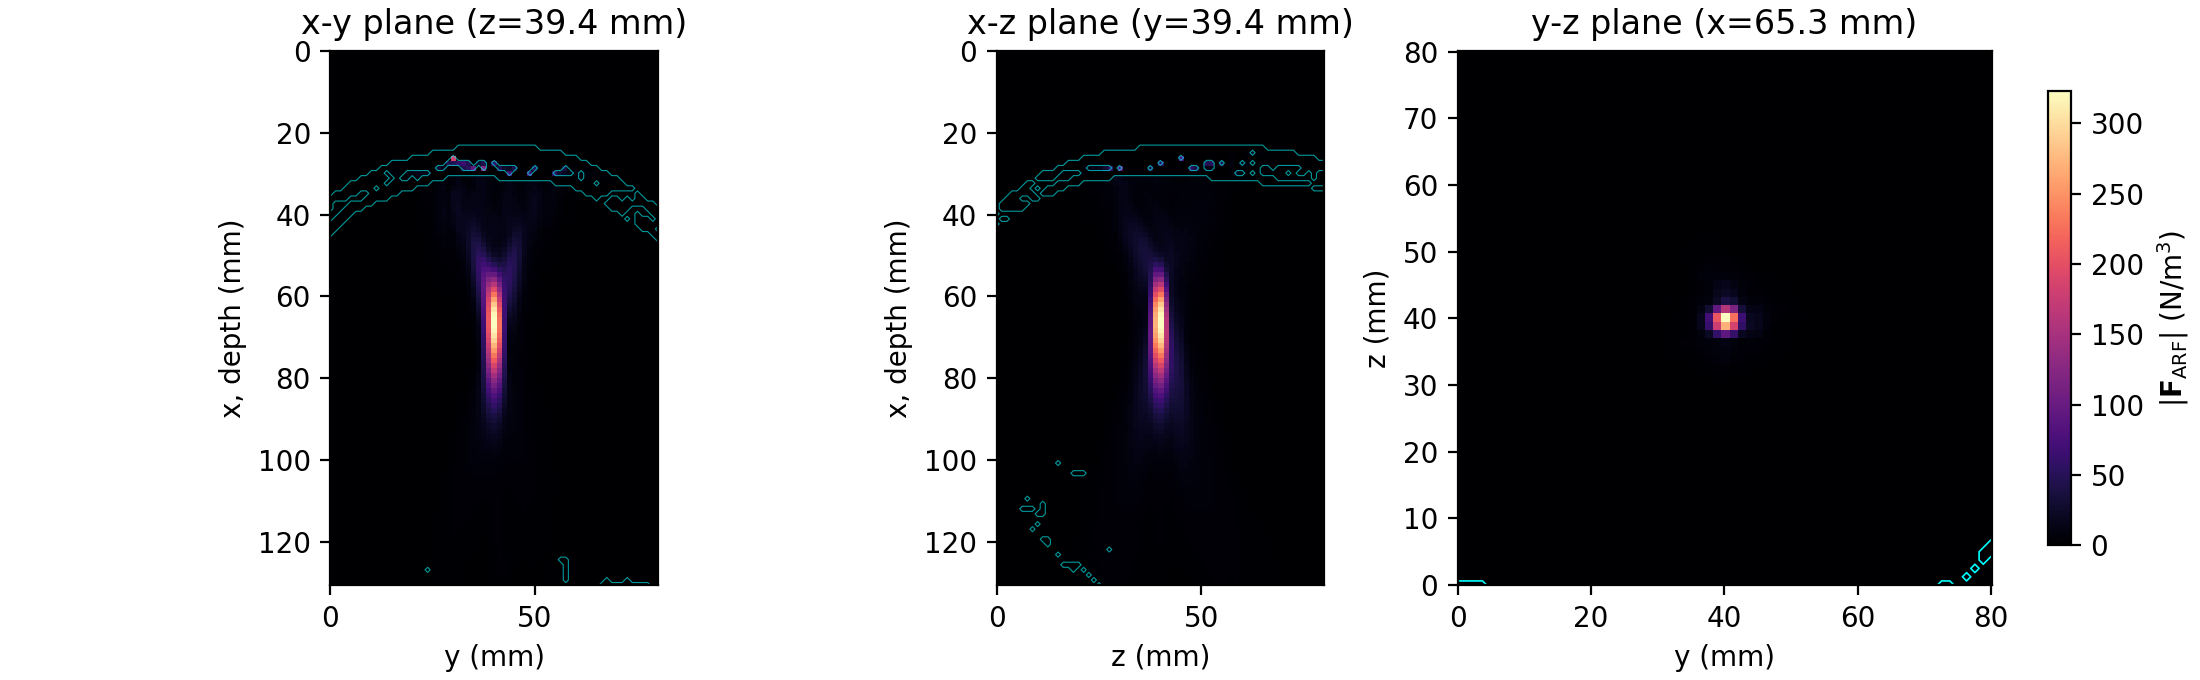
\includegraphics[width=\linewidth]{elastic_arf_ortho.png}
\caption{Orthogonal slices of the ARF body-force density $|\mathbf{F}_{\mathrm{ARF}}|$ through the brain-restricted peak voxel.  ARF is the acoustic body force that drives the displacement trace and snapshots in the following two subsections.  Cyan contour shows the skull mask ($c>1600$\,m/s).}\label{fig:arf_ortho}
\end{figure}

\subsection{ARF density — 3-D rendering}\label{sec:arf_3d}
\begin{figure}[H]\centering
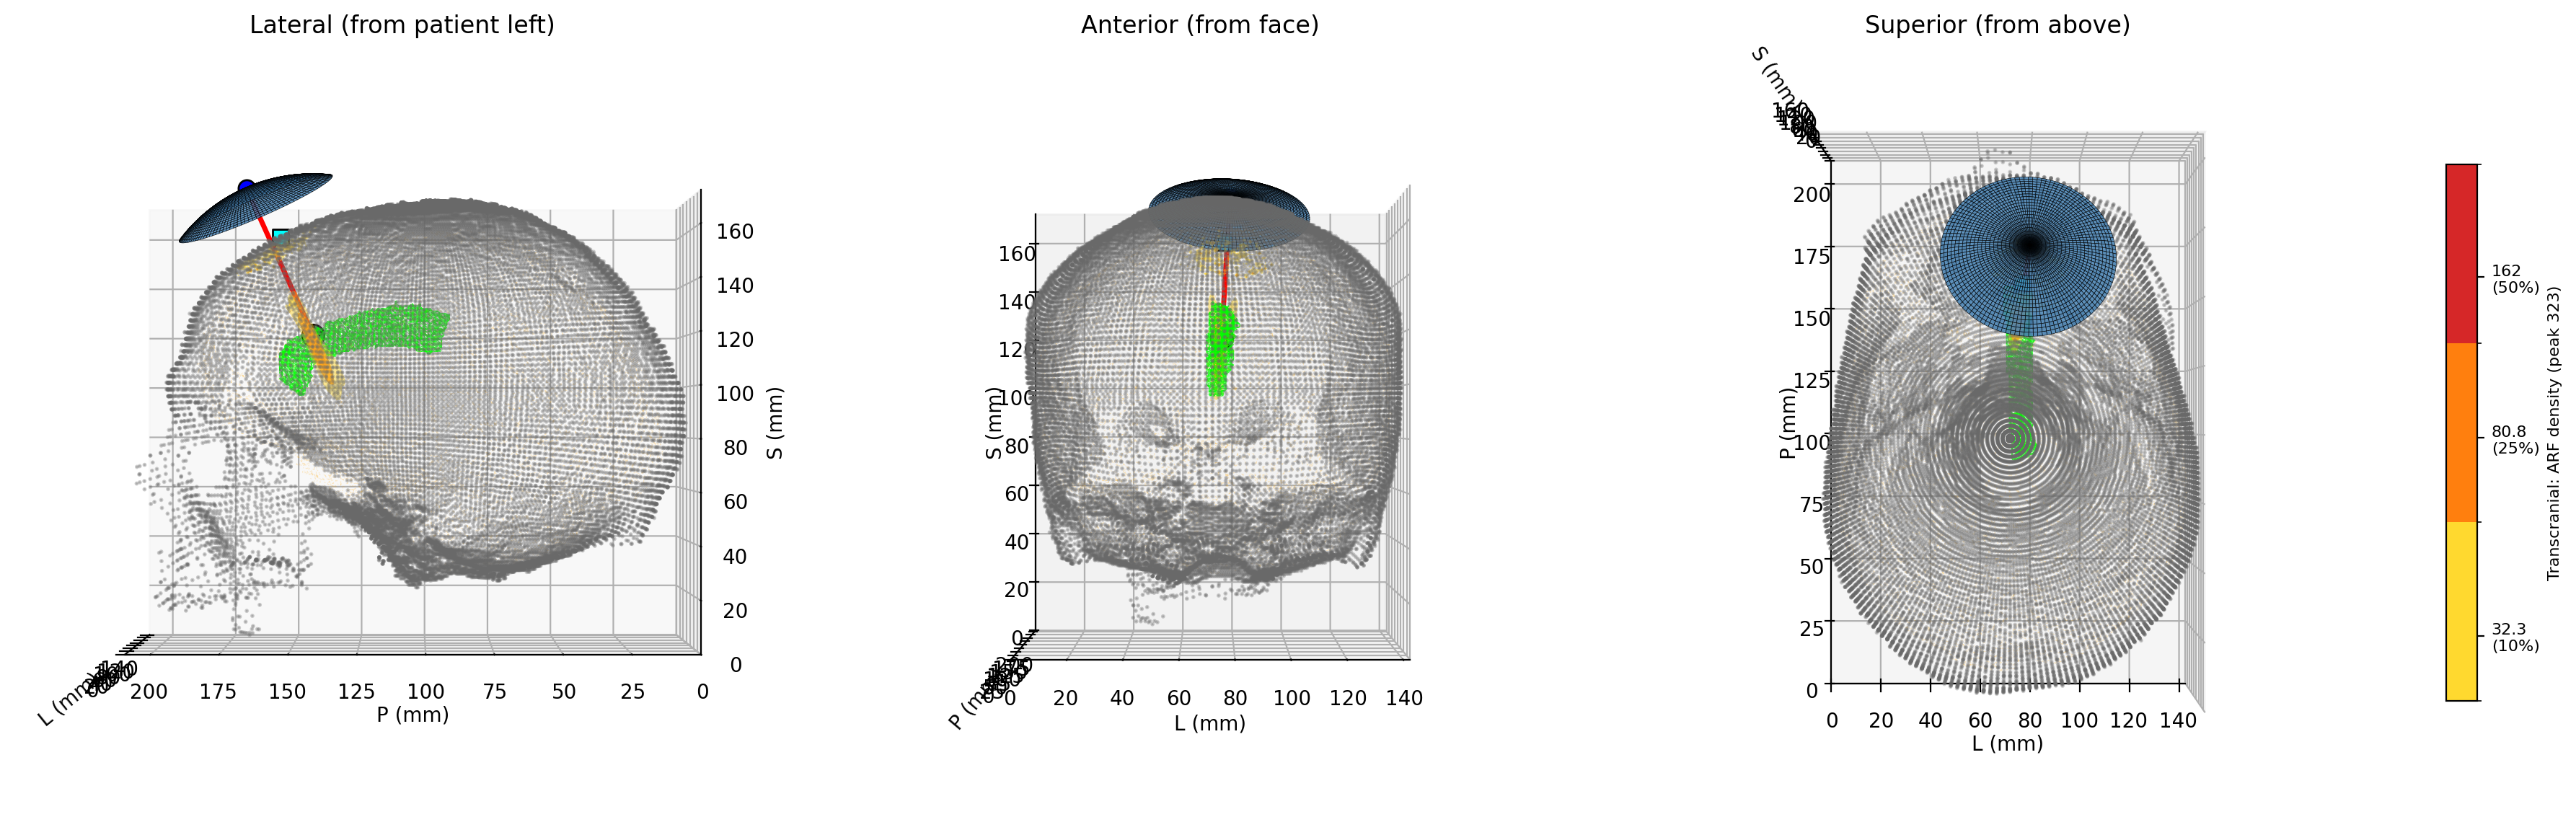
\includegraphics[width=\linewidth]{elastic_arf_3d.png}
\caption{Three-camera 3-D rendering of the ARF body-force density patterned on Fig.~\ref{fig:thermal_3d}: full skull point cloud, pial brain mesh, target ROI, bowl wireframe, beam axis, and apex/scalp/target/focus markers in LPS, with iso-surfaces at 50\,\% / 25\,\% / 10\,\% of peak overlaid.  Three views: lateral, anterior, superior.}\label{fig:arf_3d}
\end{figure}


\subsection{Displacement at peak ARF voxel}\label{sec:displacement_trace}
\begin{figure}[H]\centering
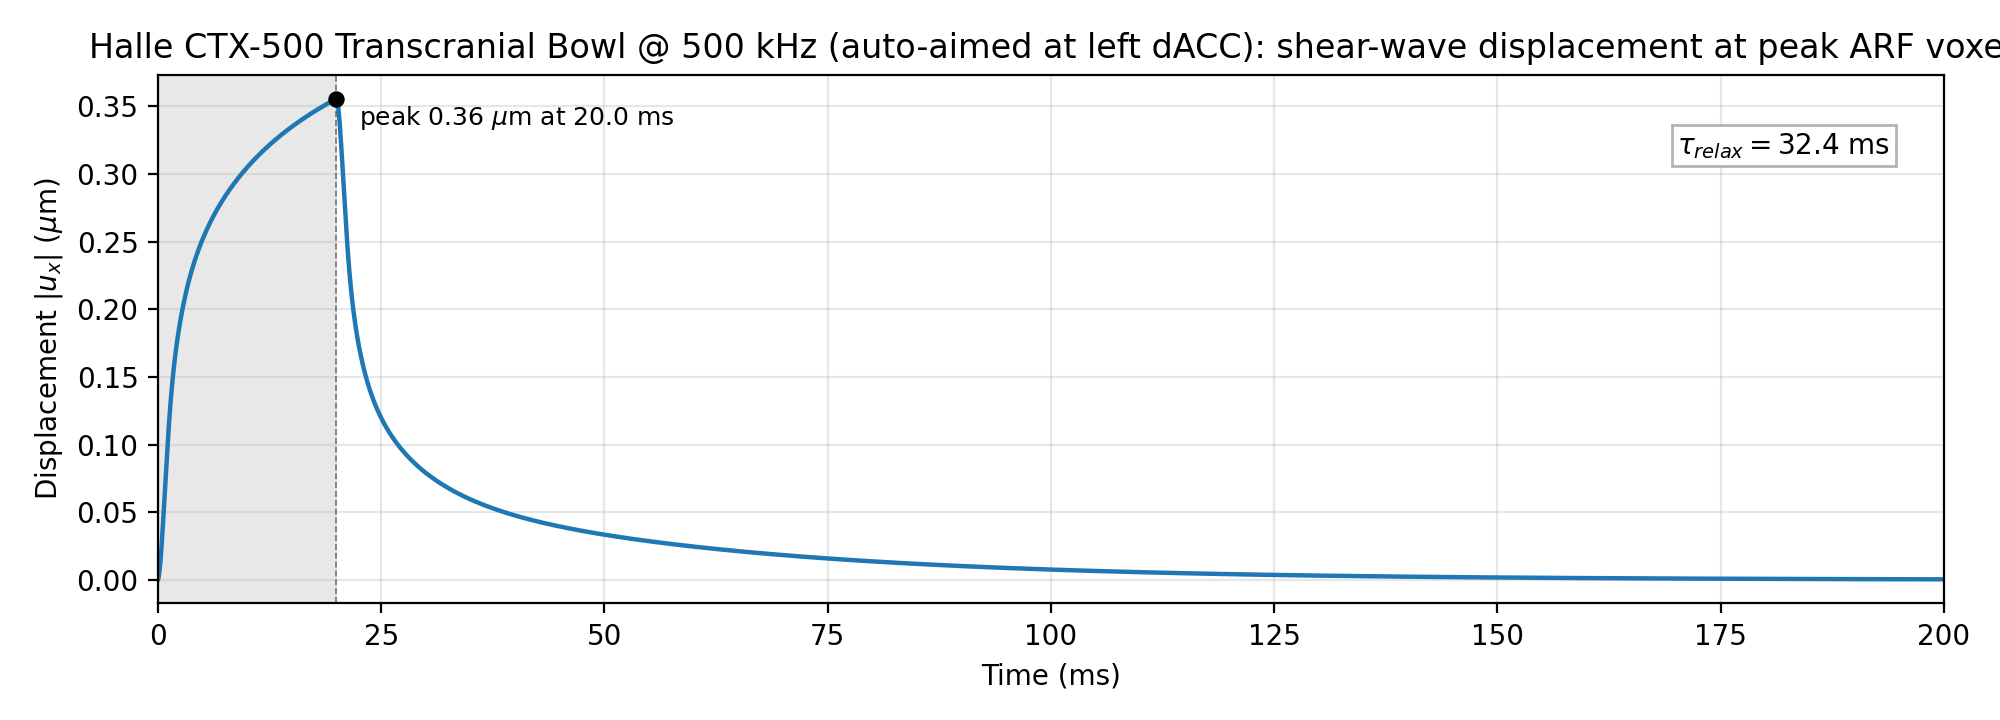
\includegraphics[width=\linewidth]{fig_disp_trace.png}
\caption{$|u_x|$ at the peak ARF voxel over one PRF period.  The shaded band marks the 20\,ms ON window during which the gated radiation force pushes the medium; the unshaded 180\,ms OFF window shows the visco-elastic relaxation back toward zero displacement.  $\tau$ is fit by linear regression of $\log |u_x|$ against $t$ on the OFF segment.}\label{fig:displacement_trace}
\end{figure}

\subsection{Snapshots through peak ARF voxel}\label{sec:displacement_snapshots}
\begin{figure}[H]\centering
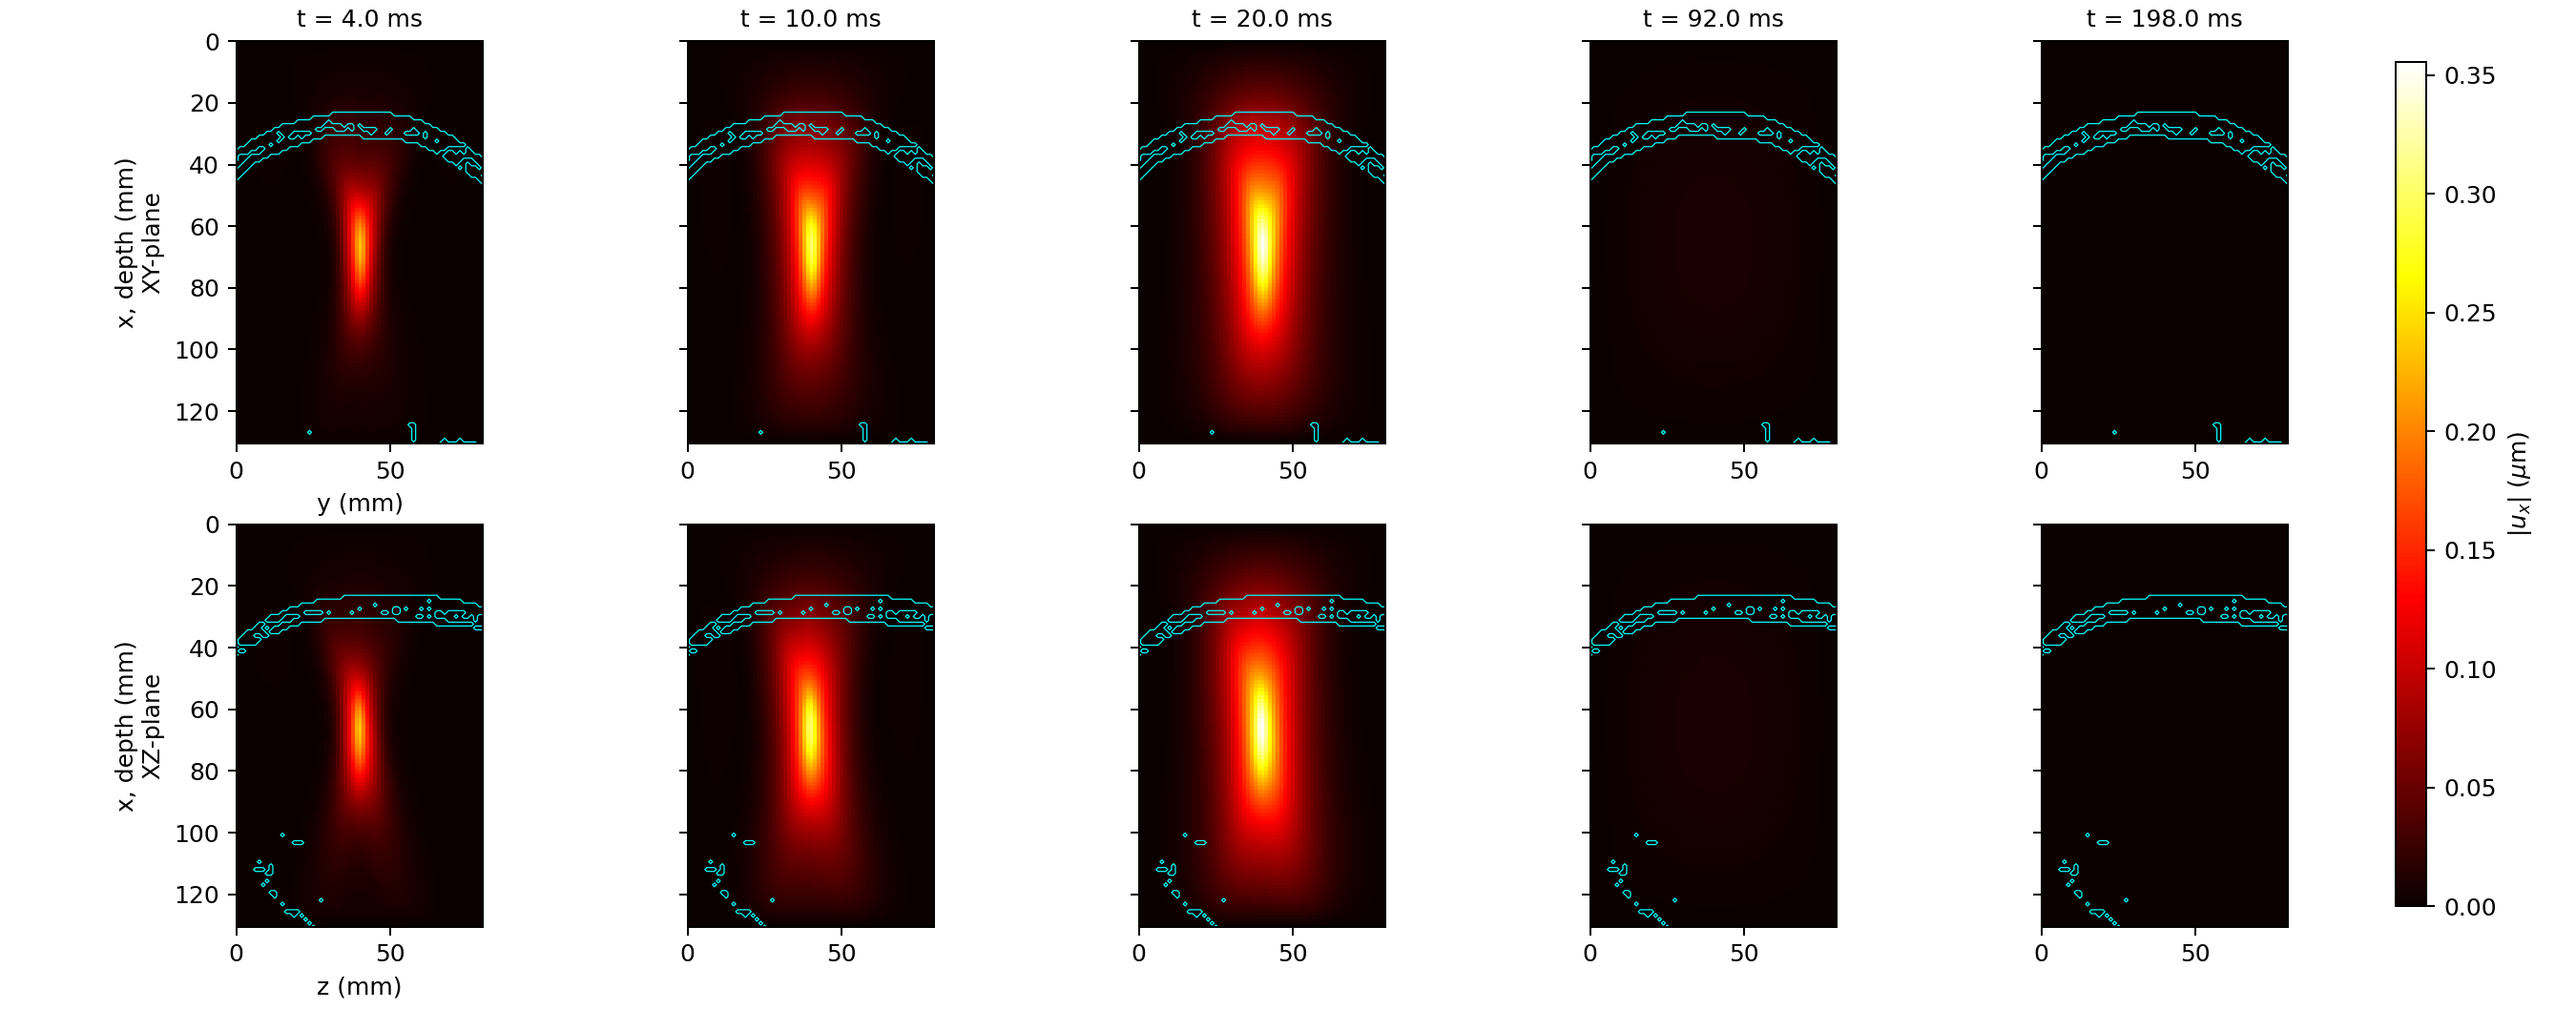
\includegraphics[width=\linewidth]{fig_disp_snapshots.png}
\caption{$|u_x|$ snapshots on the XY (top) and XZ (bottom) planes through the peak ARF voxel at five representative times spanning one PRF period.  The first three columns sample the ON ramp-up; the last two the OFF relaxation.  Cyan contours mark the skull mask ($c > 1700$\,m/s).  All panels share the colourmap (right).}\label{fig:displacement_snapshots}
\end{figure}







\section{Elastic Outputs}\label{sec:elastic_outputs}


The static elastic equilibrium driven by the acoustic radiation force
$\mathbf{F}_{\mathrm{ARF}} = 2\alpha \mathbf{I}/c$ is solved on the same
downsampled validation grid as Sections~\ref{sec:acoustic_outputs}
and~\ref{sec:thermal_outputs}.  Three voxelwise scalar fields are
reported: (i) the ARF body-force magnitude itself, (ii) the equivalent
deviatoric (von Mises) strain
$\varepsilon_{\mathrm{eq}} = \sqrt{\tfrac{2}{3}\,\varepsilon^{\mathrm{dev}}_{ij}\varepsilon^{\mathrm{dev}}_{ij}}$
computed from the displacement field by central differences on the
strain tensor, and (iii) the membrane tension
$T = K_A\,\alpha\,\varepsilon_{\mathrm{eq}}$
with the lipid-bilayer area-expansion
modulus $K_A = 0.25$~N/m and
the multi-scale coupling factor $\alpha = 1000$
(same convention as the neural section, so the elastic and neural
tension renderings are directly comparable).  Each field is
shown as three orthogonal slices through its brain-restricted peak
voxel (depth on the vertical axis, $0$ at the top), followed by a
three-camera 3-D iso-surface rendering.

\begin{table}[h!]
\centering
\scriptsize
\setlength{\tabcolsep}{6pt}
\renewcommand{\arraystretch}{1.05}
\begin{tabular}{lrrrl}
\toprule
\textbf{Quantity} & \textbf{Peak (full)} & \textbf{Peak (brain only)} & \textbf{Peak (skull)} & \textbf{Unit} \\
\midrule
$|\mathbf{F}_{\mathrm{ARF}}|$              & 3.230e+02     & 3.230e+02     & 1.806e+01     & N/m$^3$ \\
$\varepsilon_{\mathrm{eq}}$                & 2.313e-05  & 2.313e-05  & 0.000e+00  & — \\
$T = K_a\,|\varepsilon_{\mathrm{vol}}|$    & 5.782e+00 & 5.782e+00 & 0.000e+00 & N/m \\
\bottomrule
\end{tabular}
\caption{Peak elastic-output magnitudes from the static shear-FDTD equilibrium.  The brain-only column excludes voxels with $c>1600$\,m/s; ARF concentrates in skull due to absorption while strain and tension peak near the focal lobe.}\label{tab:elastic_outputs}
\end{table}

\subsection{Equivalent deviatoric strain — three-plane views}\label{sec:strain_ortho}
\begin{figure}[H]\centering
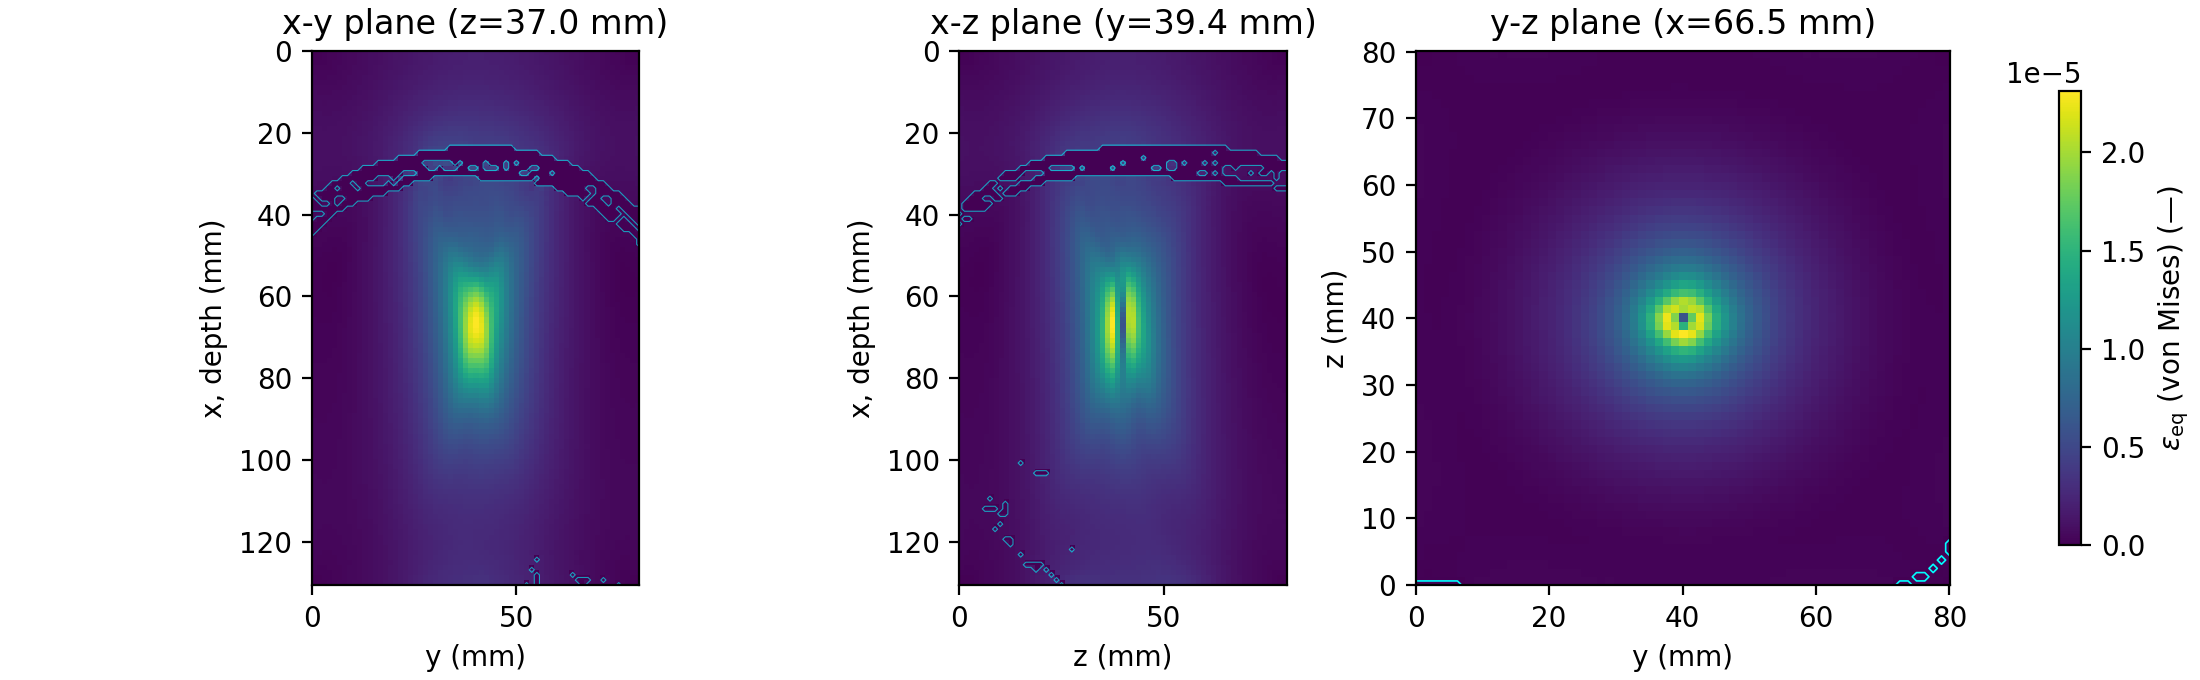
\includegraphics[width=\linewidth]{elastic_strain_ortho.png}
\caption{Orthogonal slices of the equivalent deviatoric strain $\varepsilon_{\mathrm{eq}}$ through its brain-restricted peak voxel.  Skull voxels ($c>1600$ m/s) are masked to zero before peak finding and rendering, since the shear-FDTD elastic discontinuity at the skull-brain boundary produces large spurious gradients there.}\label{fig:strain_ortho}
\end{figure}



\subsection{Equivalent deviatoric strain — tensor snapshots}\label{sec:eeq_time}
\begin{figure}[H]\centering
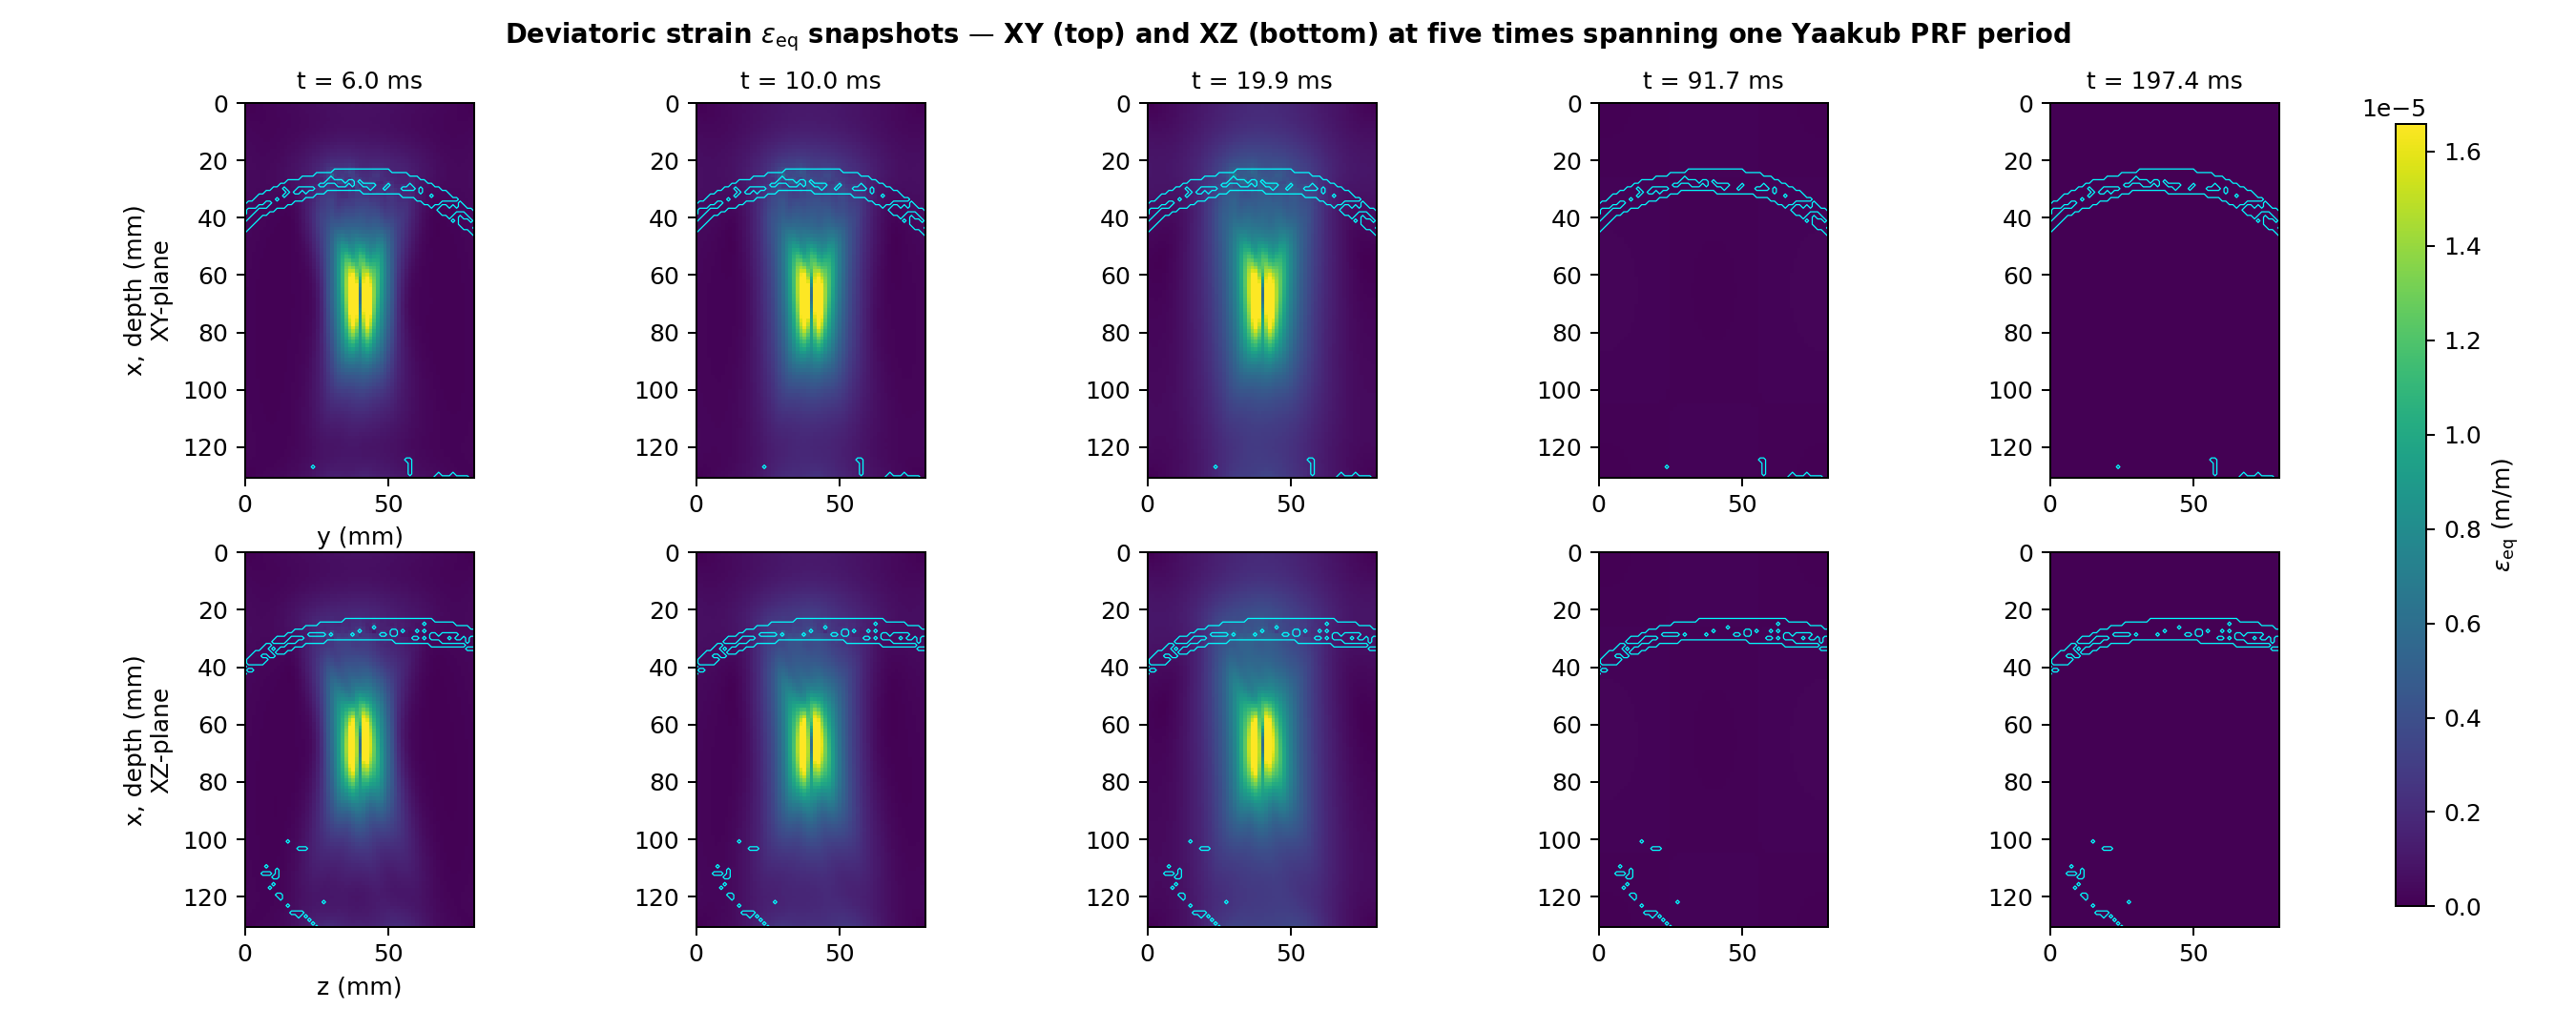
\includegraphics[width=\linewidth]{elastic_eeq_time.png}
\caption{True deviatoric strain tensor $\varepsilon_{\mathrm{eq}} = \sqrt{\tfrac{2}{3}\,\varepsilon^{\mathrm{dev}}_{ij}\varepsilon^{\mathrm{dev}}_{ij}}$ at five times spanning one Yaakub PRF period, computed by central differences on the full 3-D displacement trajectory ``displacement\_4d.npy''.  Three columns trace the ON ramp-up; the last two trace the OFF relaxation.  Top row: $x$--$y$ slice at mid elevation; bottom: $x$--$z$ slice at mid lateral.  Cyan contour: skull mask.  Field-wide max $\varepsilon_{\mathrm{eq}} = 2.31e-05$.}\label{fig:eeq_time}
\end{figure}




\subsection{Membrane tension — tensor snapshots}\label{sec:tension_time}
\begin{figure}[H]\centering
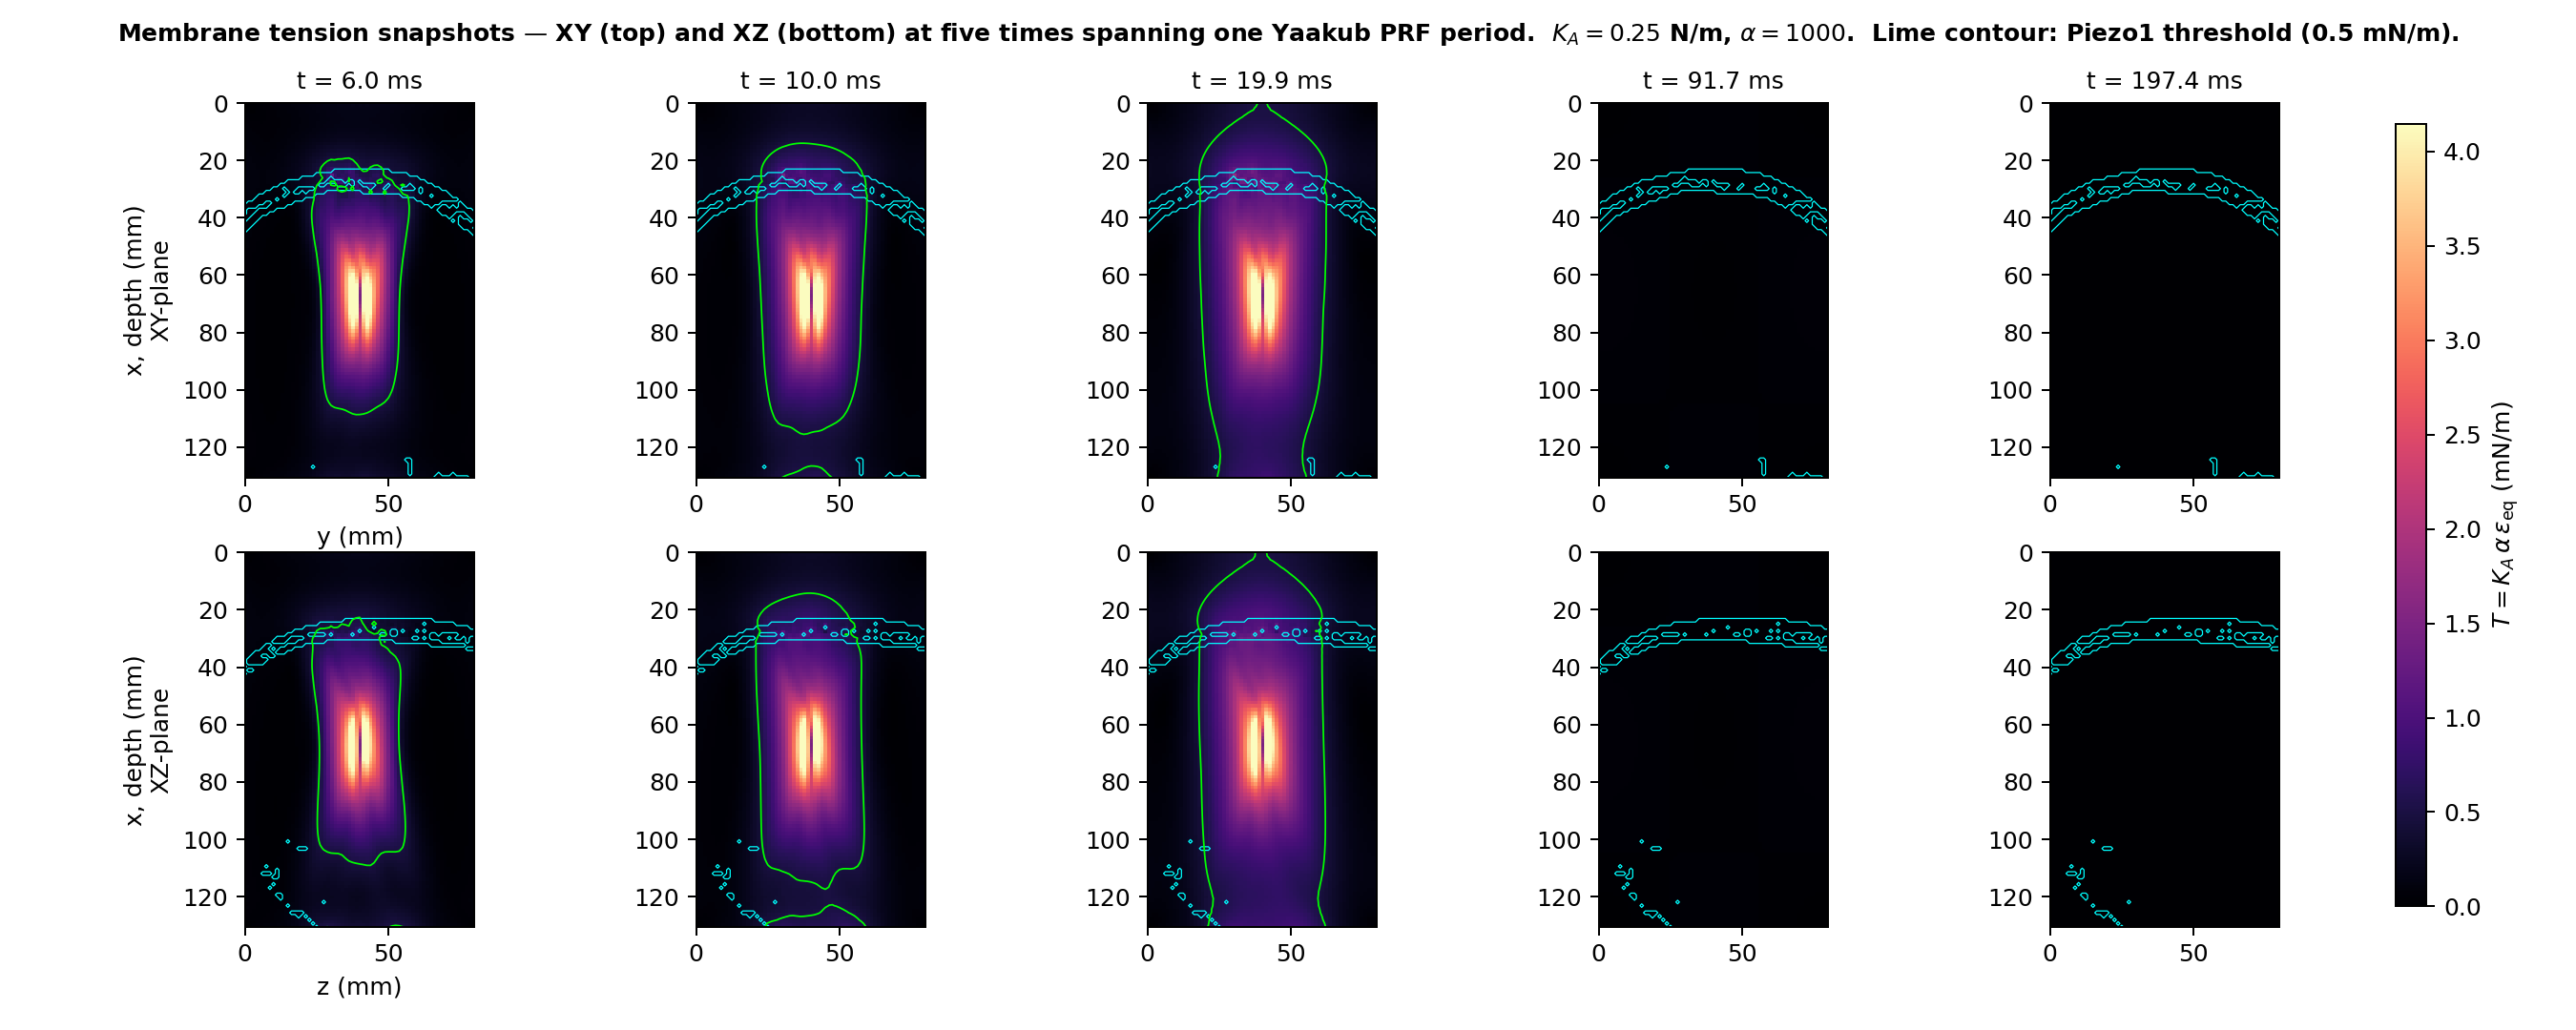
\includegraphics[width=\linewidth]{elastic_tension_time.png}
\caption{Membrane tension $T = K_A\,\alpha\,\varepsilon_{\mathrm{eq}}$ at the same five times as Fig.~\ref{fig:eeq_time}, with $K_A = 0.25$\,N/m and the multi-scale tissue\,$\to$\,membrane coupling factor $\alpha = 1000$.  Cyan contour: skull mask.  Lime contour: Piezo1 firing threshold (0.5\,mN/m).  Field-wide max $T = 5.78$\,mN/m.}\label{fig:tension_time}
\end{figure}





\subsection{Passive-membrane depolarisation $\Delta V$}\label{sec:depolarization}
The conductance-weighted steady-state depolarisation per voxel,
$\Delta V_{\mathrm{passive}} = V_{\mathrm{ss}}(T(\mathbf{x})) - V_{\mathrm{rest}}$, is a cell-type-independent readout: the firing-zone for any spike threshold drops out as the iso-surface $\Delta V = V_{\mathrm{thresh}} - V_{\mathrm{rest}}$ set by the cell substrate (e.g. $\sim$+15\,mV for cortical-pyramidal AIS, $\sim$+8\,mV for fast-spiking interneurons).  Computed analytically from the static-equilibrium tension field with Piezo1 ($\bar{g} = 0.10$\,mS/cm$^2$, $E_{\mathrm{rev}} = 0$\,mV), TREK-1 ($\bar{g} = 0.04$\,mS/cm$^2$, $E_{\mathrm{rev}} = -90$\,mV), and the Pospischil cortical leak ($\bar{g}_L = 0.0167$\,mS/cm$^2$, $E_L = -70.3$\,mV).  Brain-peak $\Delta V_{\mathrm{passive}} = 52.99$\,mV.

\begin{figure}[H]\centering
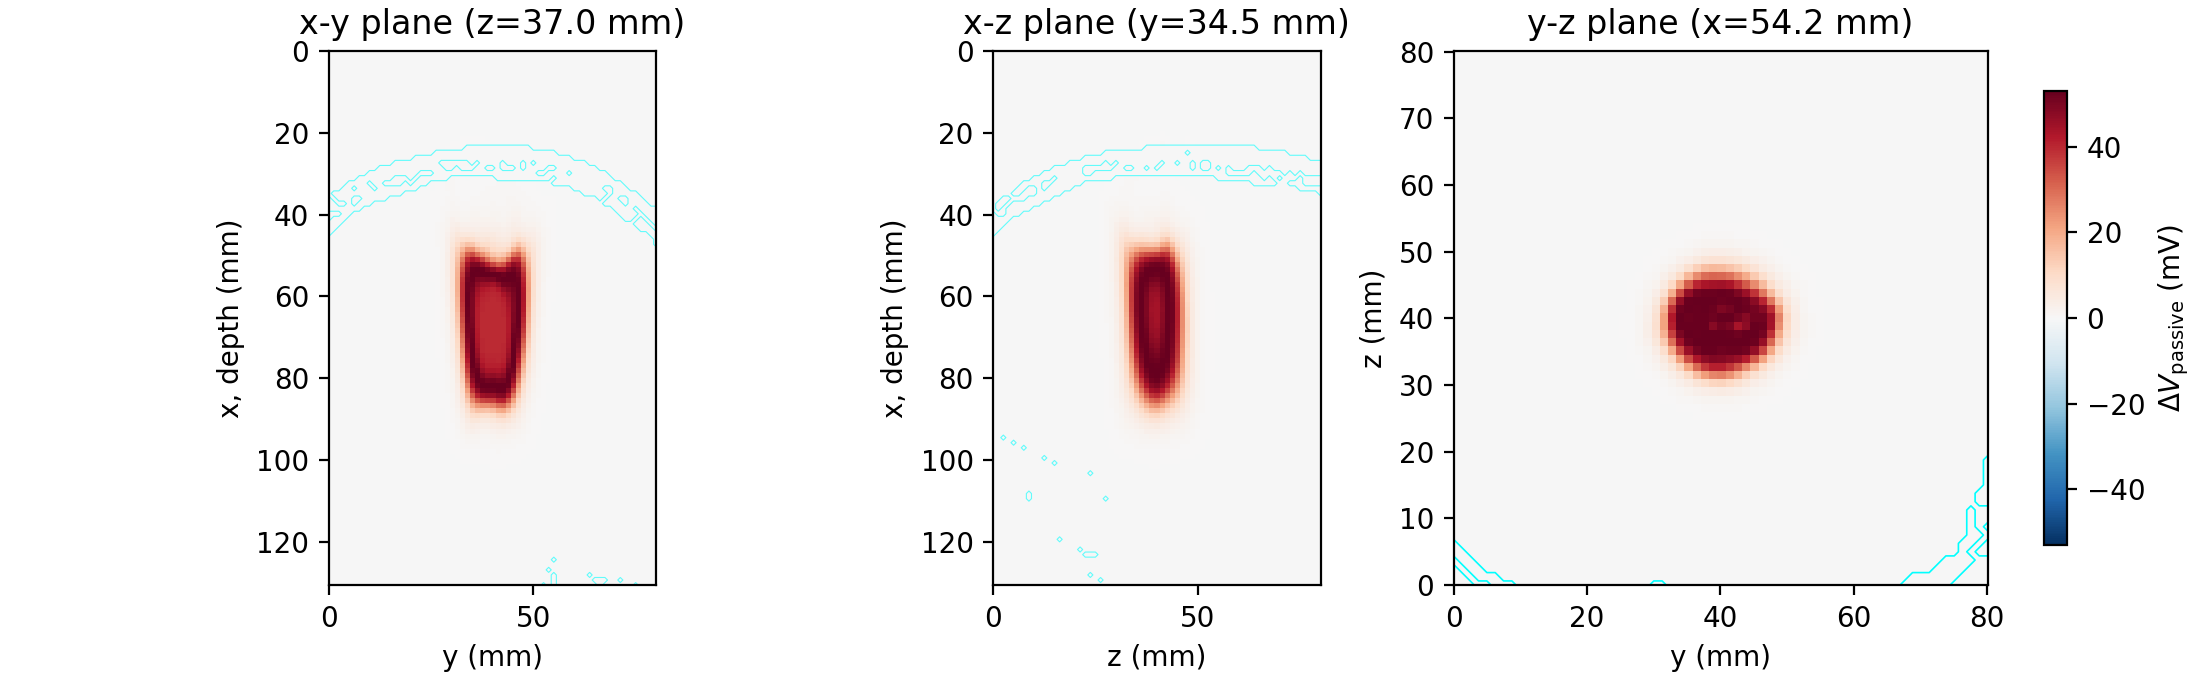
\includegraphics[width=\linewidth]{elastic_depolarization_ortho.png}
\caption{Passive-membrane $\Delta V_{\mathrm{passive}}$ on three orthogonal slices through the brain-restricted peak voxel.  Diverging colourmap with zero centred so depolarising and (TREK-1-driven) hyperpolarising contributions are both visible; cyan contour: skull mask.}\label{fig:depolarization_ortho}
\end{figure}

\begin{figure}[H]\centering
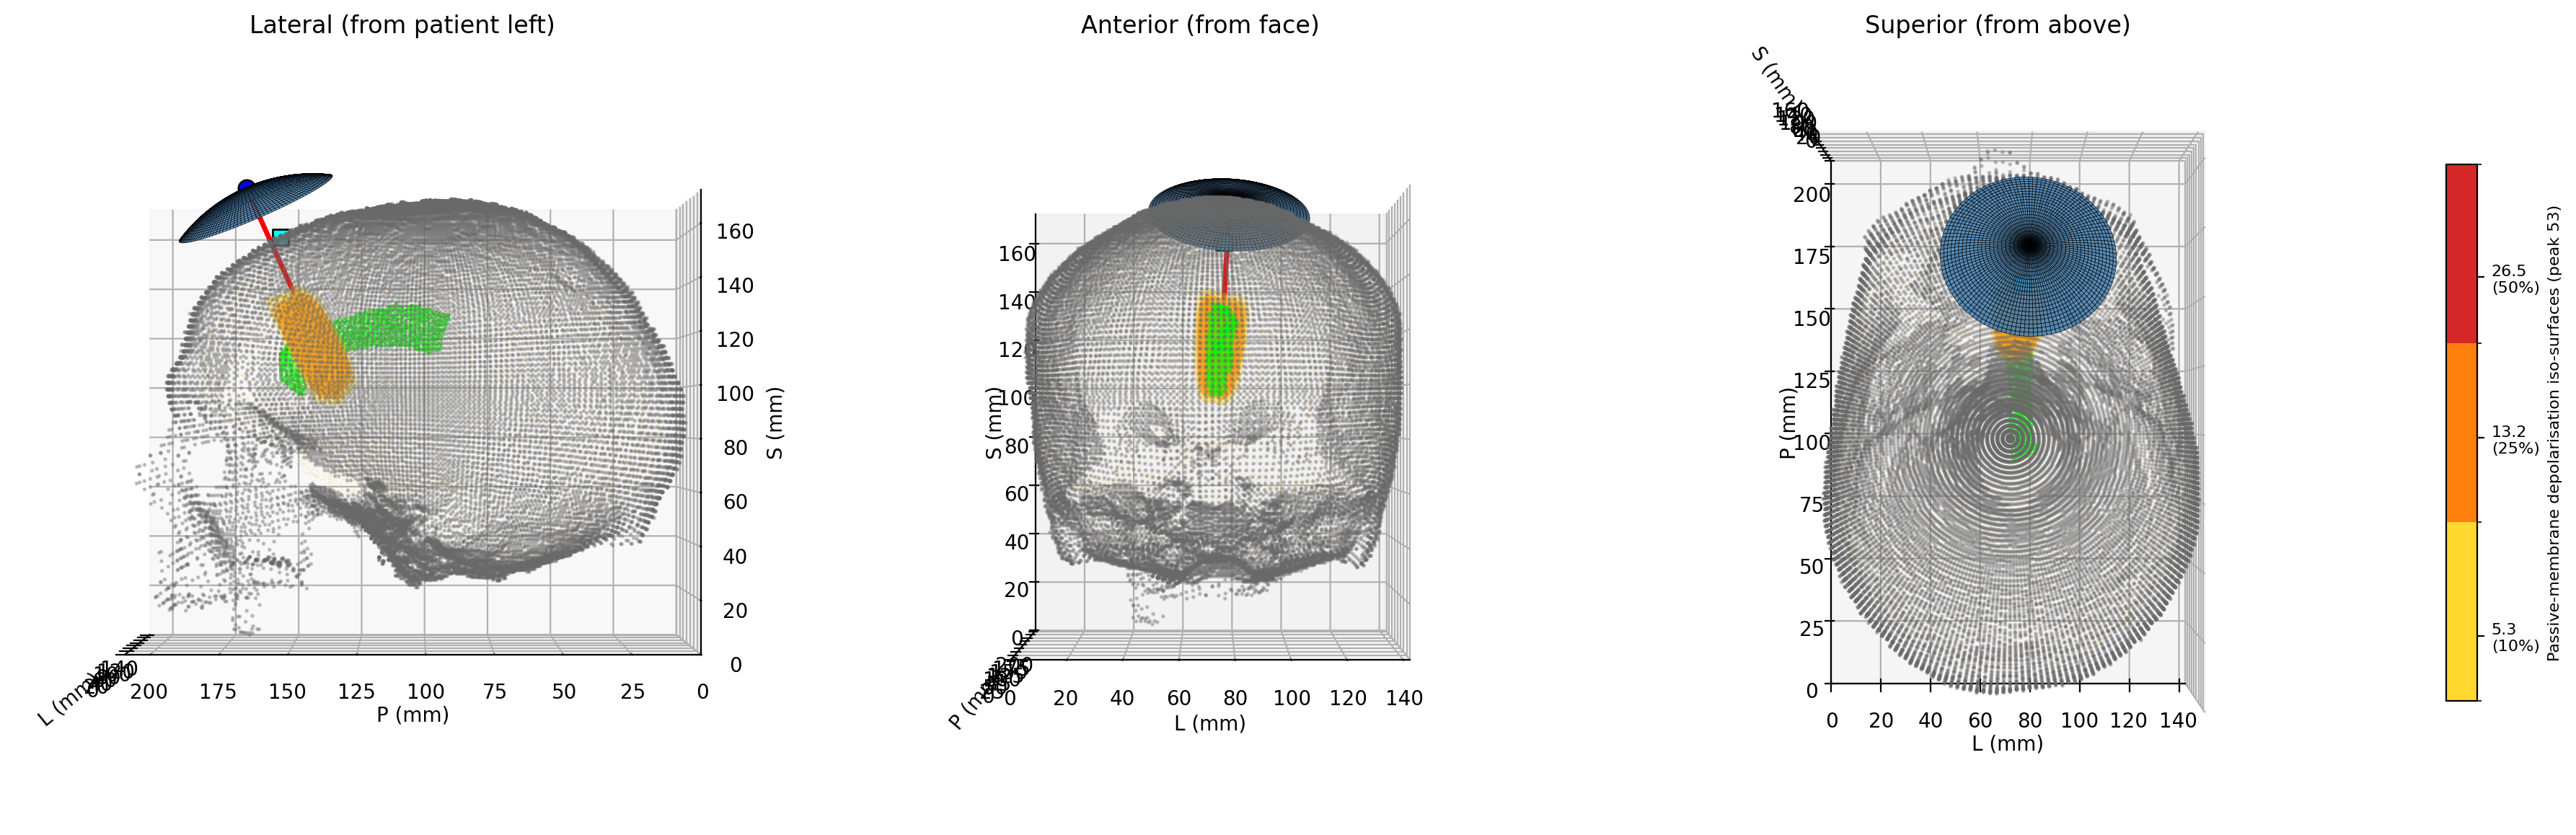
\includegraphics[width=\linewidth]{elastic_depolarization_3d.png}
\caption{Three-camera 3-D rendering of the depolarisation field with iso-surfaces at 50\,\% / 25\,\% / 10\,\% of the brain-peak $\Delta V_{\mathrm{passive}}$, patterned on Fig.~\ref{fig:thermal_3d}.  The 50\,\% iso-surface bounds the volume that is depolarised at least halfway to the focal-voxel maximum; readers can map any cell-type-specific spike threshold to the corresponding iso-level on this continuous field.}\label{fig:depolarization_3d}
\end{figure}


\subsection{Equivalent deviatoric strain — 3-D rendering}\label{sec:strain_3d}
\begin{figure}[H]\centering
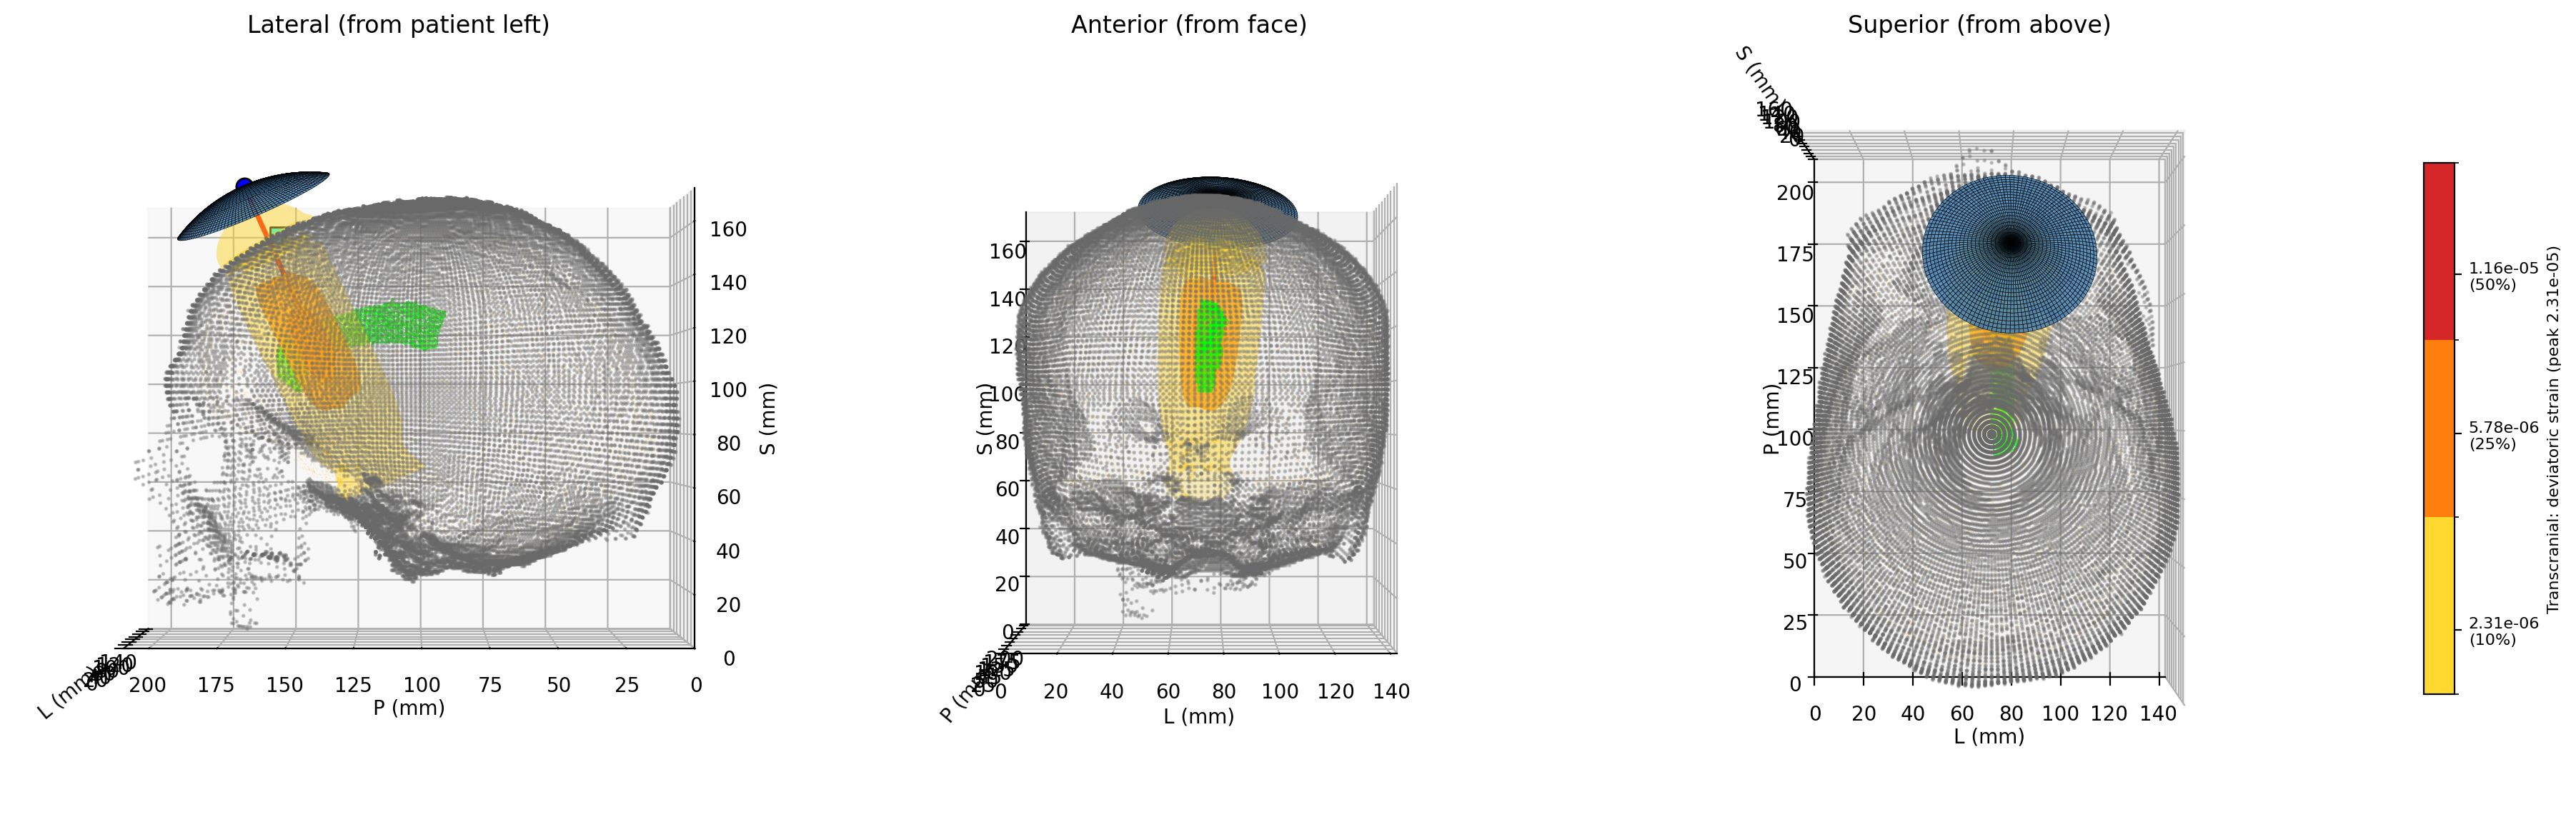
\includegraphics[width=\linewidth]{elastic_strain_3d.png}
\caption{Three-camera 3-D rendering of $\varepsilon_{\mathrm{eq}}$ patterned on Fig.~\ref{fig:thermal_3d}: full skull point cloud, pial brain mesh, target ROI, bowl wireframe, beam axis, and apex/scalp/target/focus markers in LPS, with iso-surfaces at 50\,\% / 25\,\% / 10\,\% of brain-peak strain overlaid.  Three views: lateral, anterior, superior.}\label{fig:strain_3d}
\end{figure}

\subsection{Membrane tension — three-plane views}\label{sec:tension_ortho}
\begin{figure}[H]\centering
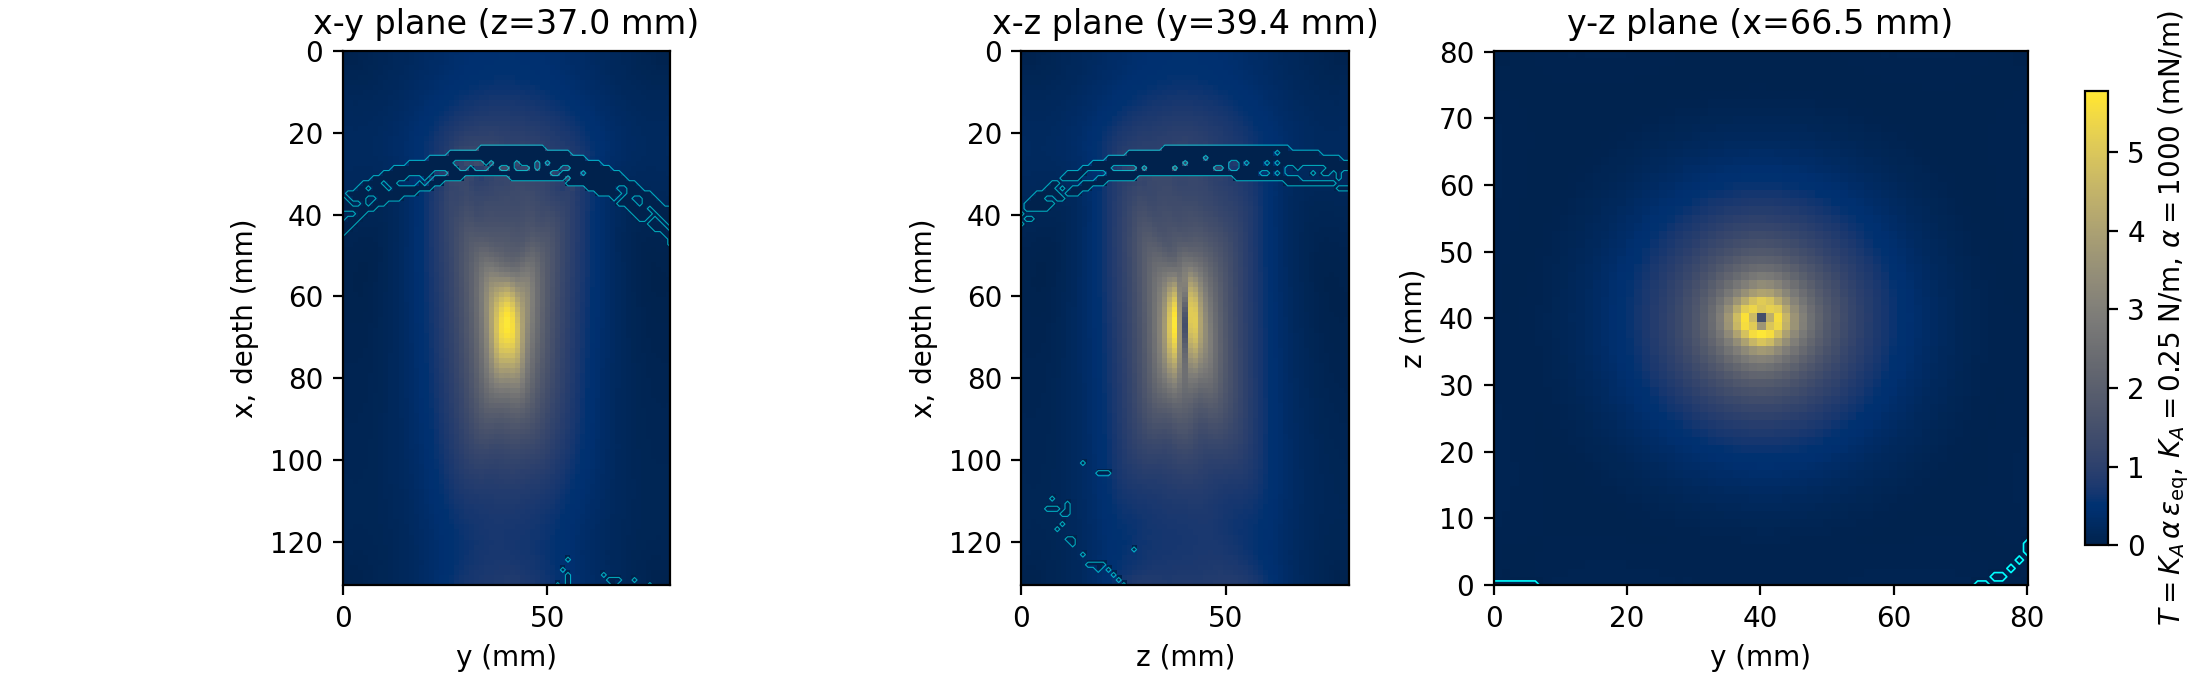
\includegraphics[width=\linewidth]{elastic_tension_ortho.png}
\caption{Orthogonal slices of the membrane-tension proxy $T = K_a\,|\varepsilon_{\mathrm{vol}}|$ through its brain-restricted peak voxel.  Skull voxels are masked to zero (the membrane-tension model applies to neuronal lipid bilayers, which exist only in brain tissue; the apparent tension at the skull-brain interface in earlier renders was a numerical-gradient artifact at the elastic discontinuity).}\label{fig:tension_ortho}
\end{figure}

\subsection{Membrane tension — 3-D rendering}\label{sec:tension_3d}
\begin{figure}[H]\centering
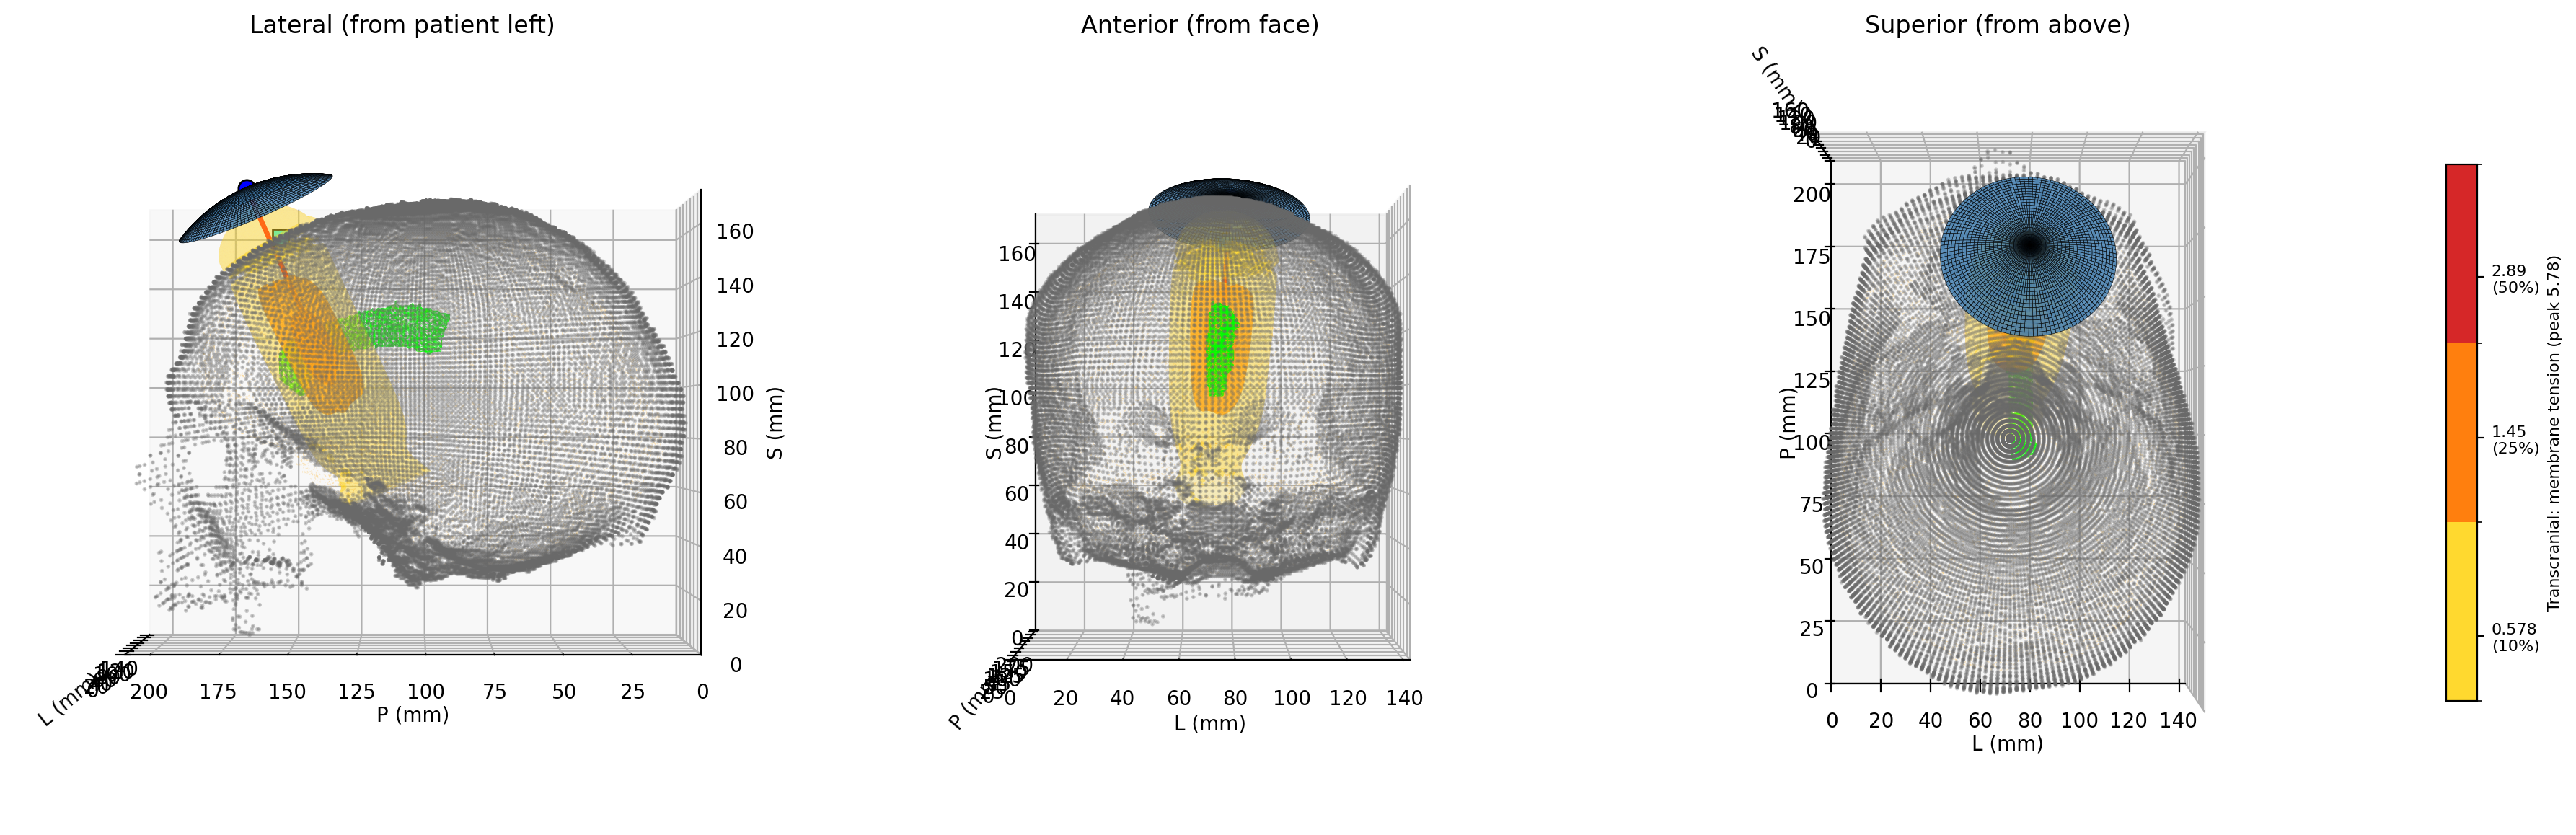
\includegraphics[width=\linewidth]{elastic_tension_3d.png}
\caption{Three-camera 3-D rendering of the membrane-tension proxy $T$ patterned on Fig.~\ref{fig:thermal_3d}: full skull point cloud, pial brain mesh, target ROI, bowl wireframe, beam axis, and apex/scalp/target/focus markers in LPS, with iso-surfaces at 50\,\% / 25\,\% / 10\,\% of the brain-peak tension overlaid.  Three views: lateral, anterior, superior.}\label{fig:tension_3d}
\end{figure}




\section{Neural Outputs}\label{sec:neural_outputs}


A 3-compartment Pinsky--Rinzel cortical pyramidal neuron
(\texttt{MulticompartmentMechanoHHNeuron.cortical\_pyramidal\_3comp})
is instantiated at every brain voxel whose peak membrane tension exceeds
0.50\,mN/m.  Peak tension is
$T = K_a\,\alpha\,\varepsilon_{\mathrm{eq}}$ with
$K_a = 0.25$\,N/m and the
multi-scale tissue\,$\to$\,membrane coupling factor
$\alpha = 1000$
(passed as \texttt{coupling\_factor} to
\texttt{strain\_to\_membrane\_tension}; lifts the voxel-scale
deviatoric strain $\varepsilon_{\mathrm{eq}}$ into the bilayer areal strain).
Peak $T$ across the field is
5.78\,mN/m.  Each neuron is driven by
a within-burst half-sine tension envelope $T(t) = T_{\mathrm{peak}}\sin(\pi t/T_{\mathrm{pulse}})$
with $T_{\mathrm{pulse}} = 20.0$\,ms (theta-burst
ON window from Section~\ref{sec:sequence}); per-voxel spike trains are recorded
over a 20\,ms window.  Session-scale figures
replay the single-burst response across 400 theta groups
($T_{\mathrm{group}} = 200$\,ms).

\begin{table}[h!]
\centering
\scriptsize
\setlength{\tabcolsep}{6pt}
\renewcommand{\arraystretch}{1.05}
\begin{tabular}{lrl}
\toprule
\textbf{Quantity} & \textbf{Value} & \textbf{Unit} \\
\midrule
Voxels above tension threshold      & 3531 & --- \\
Voxels with $\geq 1$ spike / burst  & 3531 & --- \\
Active fraction (per burst)         & 1.000 & --- \\
Peak per-voxel rate                 & 250.00 & Hz \\
Median first-spike latency          & 4.47 & ms \\
$10$th / $90$th \%ile latency       & 3.47 / 12.52 & ms \\
Mean spikes / firing voxel / burst  & 3.47 & --- \\
50\,\%-of-peak iso volume           & 4396.3 & mm$^3$ \\
25\,\%-of-peak iso volume           & 5432.2 & mm$^3$ \\
\bottomrule
\end{tabular}
\caption{Population neural-response metrics for a single theta-burst ON window.}\label{tab:neural_outputs}
\end{table}

\subsection{First-spike latency --- three-plane views}\label{sec:neural_latency}
\begin{figure}[H]\centering
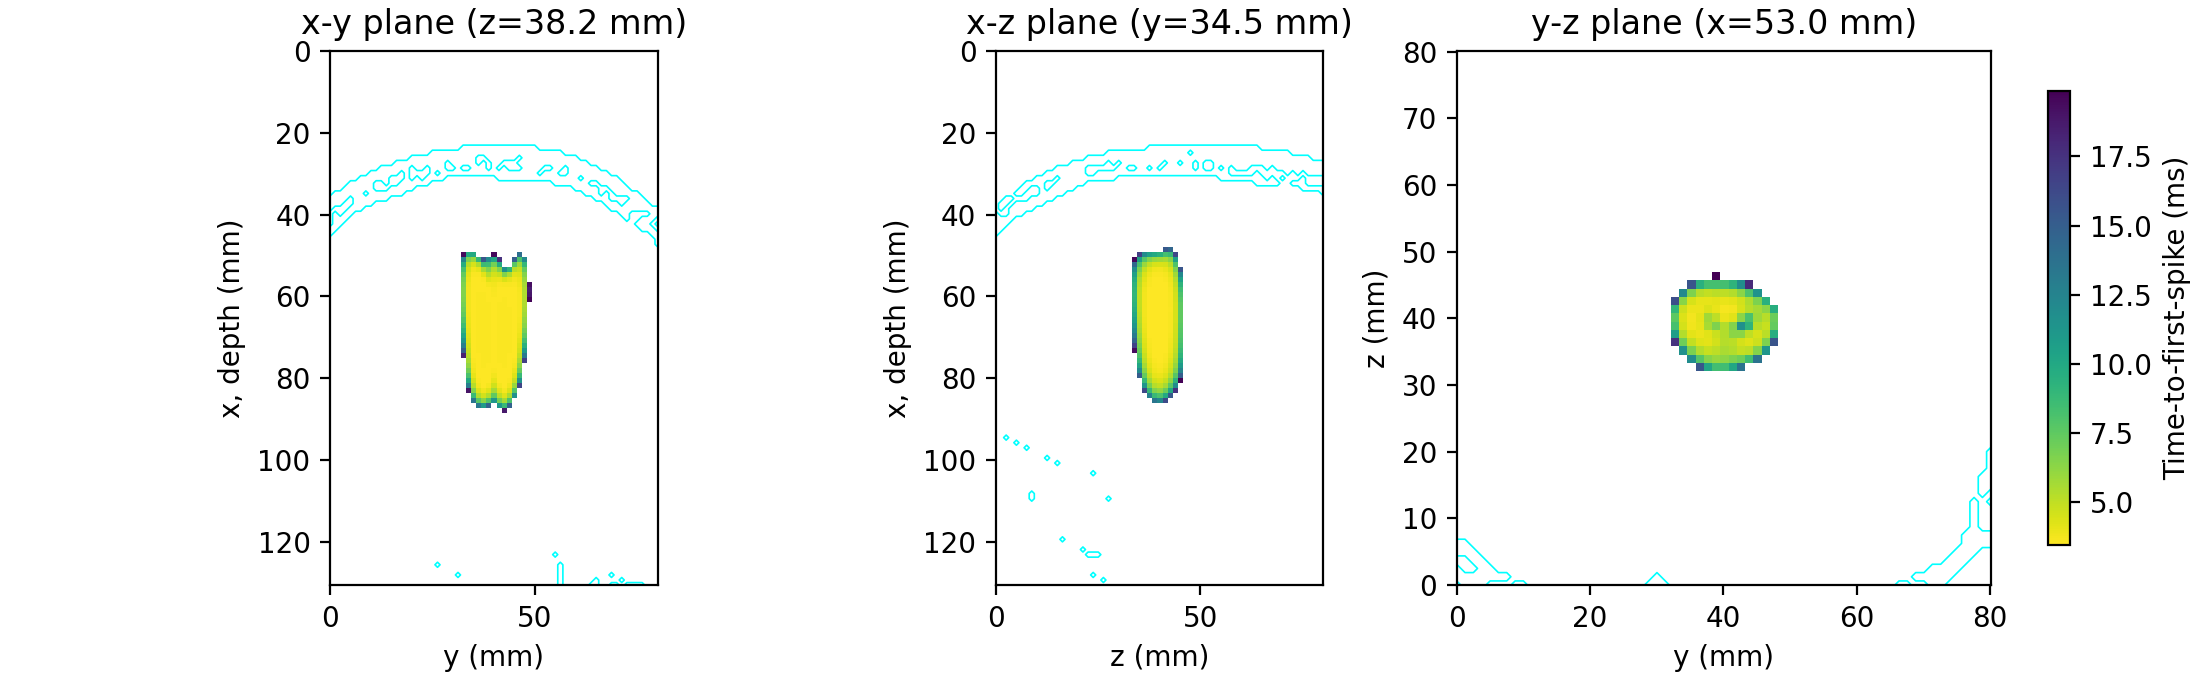
\includegraphics[width=\linewidth]{neural_latency_ortho.png}
\caption{Time-to-first-spike, brain-restricted peak voxel, three orthogonal planes (cyan: skull contour, $c>1600$\,m/s; reversed colour map so faster latencies are brighter; transparent where no spike).}\label{fig:neural_latency}
\end{figure}

\subsection{Per-voxel firing rate --- three-plane views}\label{sec:neural_rate}
\begin{figure}[H]\centering
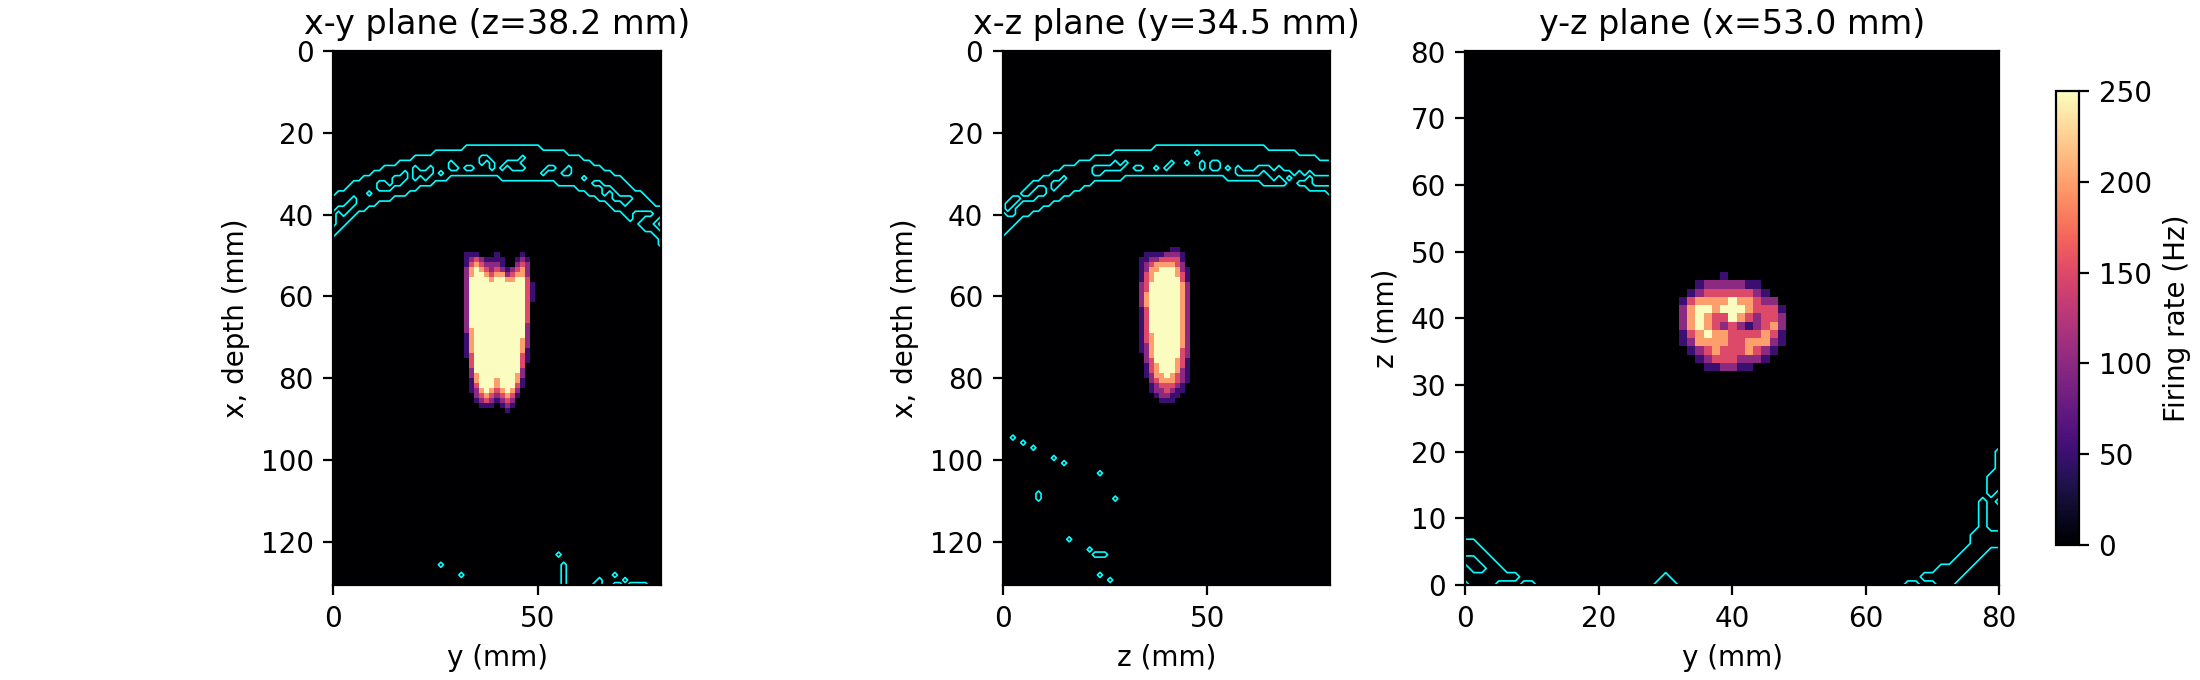
\includegraphics[width=\linewidth]{neural_rate_ortho.png}
\caption{Per-voxel firing rate (Hz) over the captured burst window, ortho slices through the brain-restricted peak.}\label{fig:neural_rate}
\end{figure}

\subsection{Three-dimensional firing iso-surfaces}\label{sec:neural_3d}
\begin{figure}[H]\centering
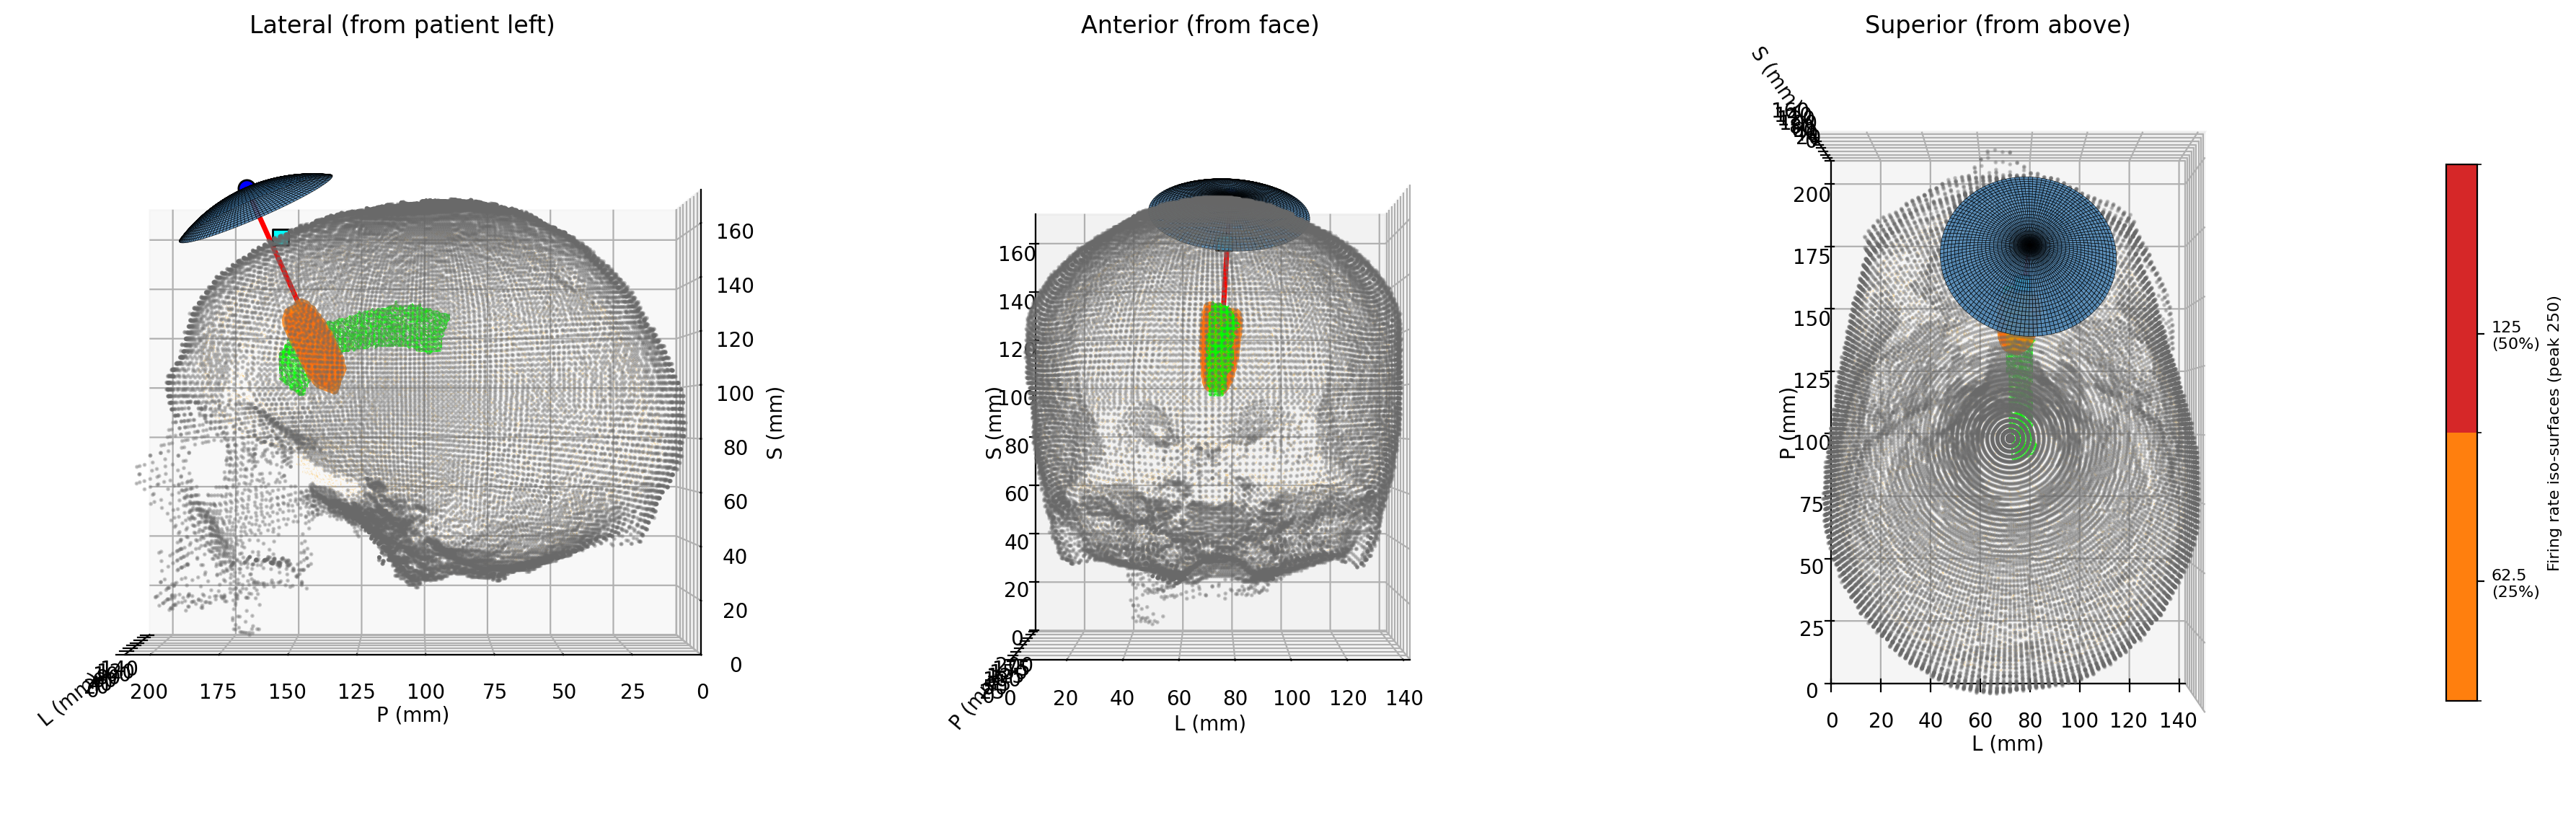
\includegraphics[width=\linewidth]{neural_rate_3d.png}
\caption{Iso-surfaces of the per-voxel firing-rate field at 50\,\% (red) and 25\,\% (orange) of peak; grey point cloud is the skull silhouette.}\label{fig:neural_3d}
\end{figure}

\subsection{Linked tension $\leftrightarrow$ spike snapshots}\label{sec:neural_snapshots}
\begin{figure}[H]\centering
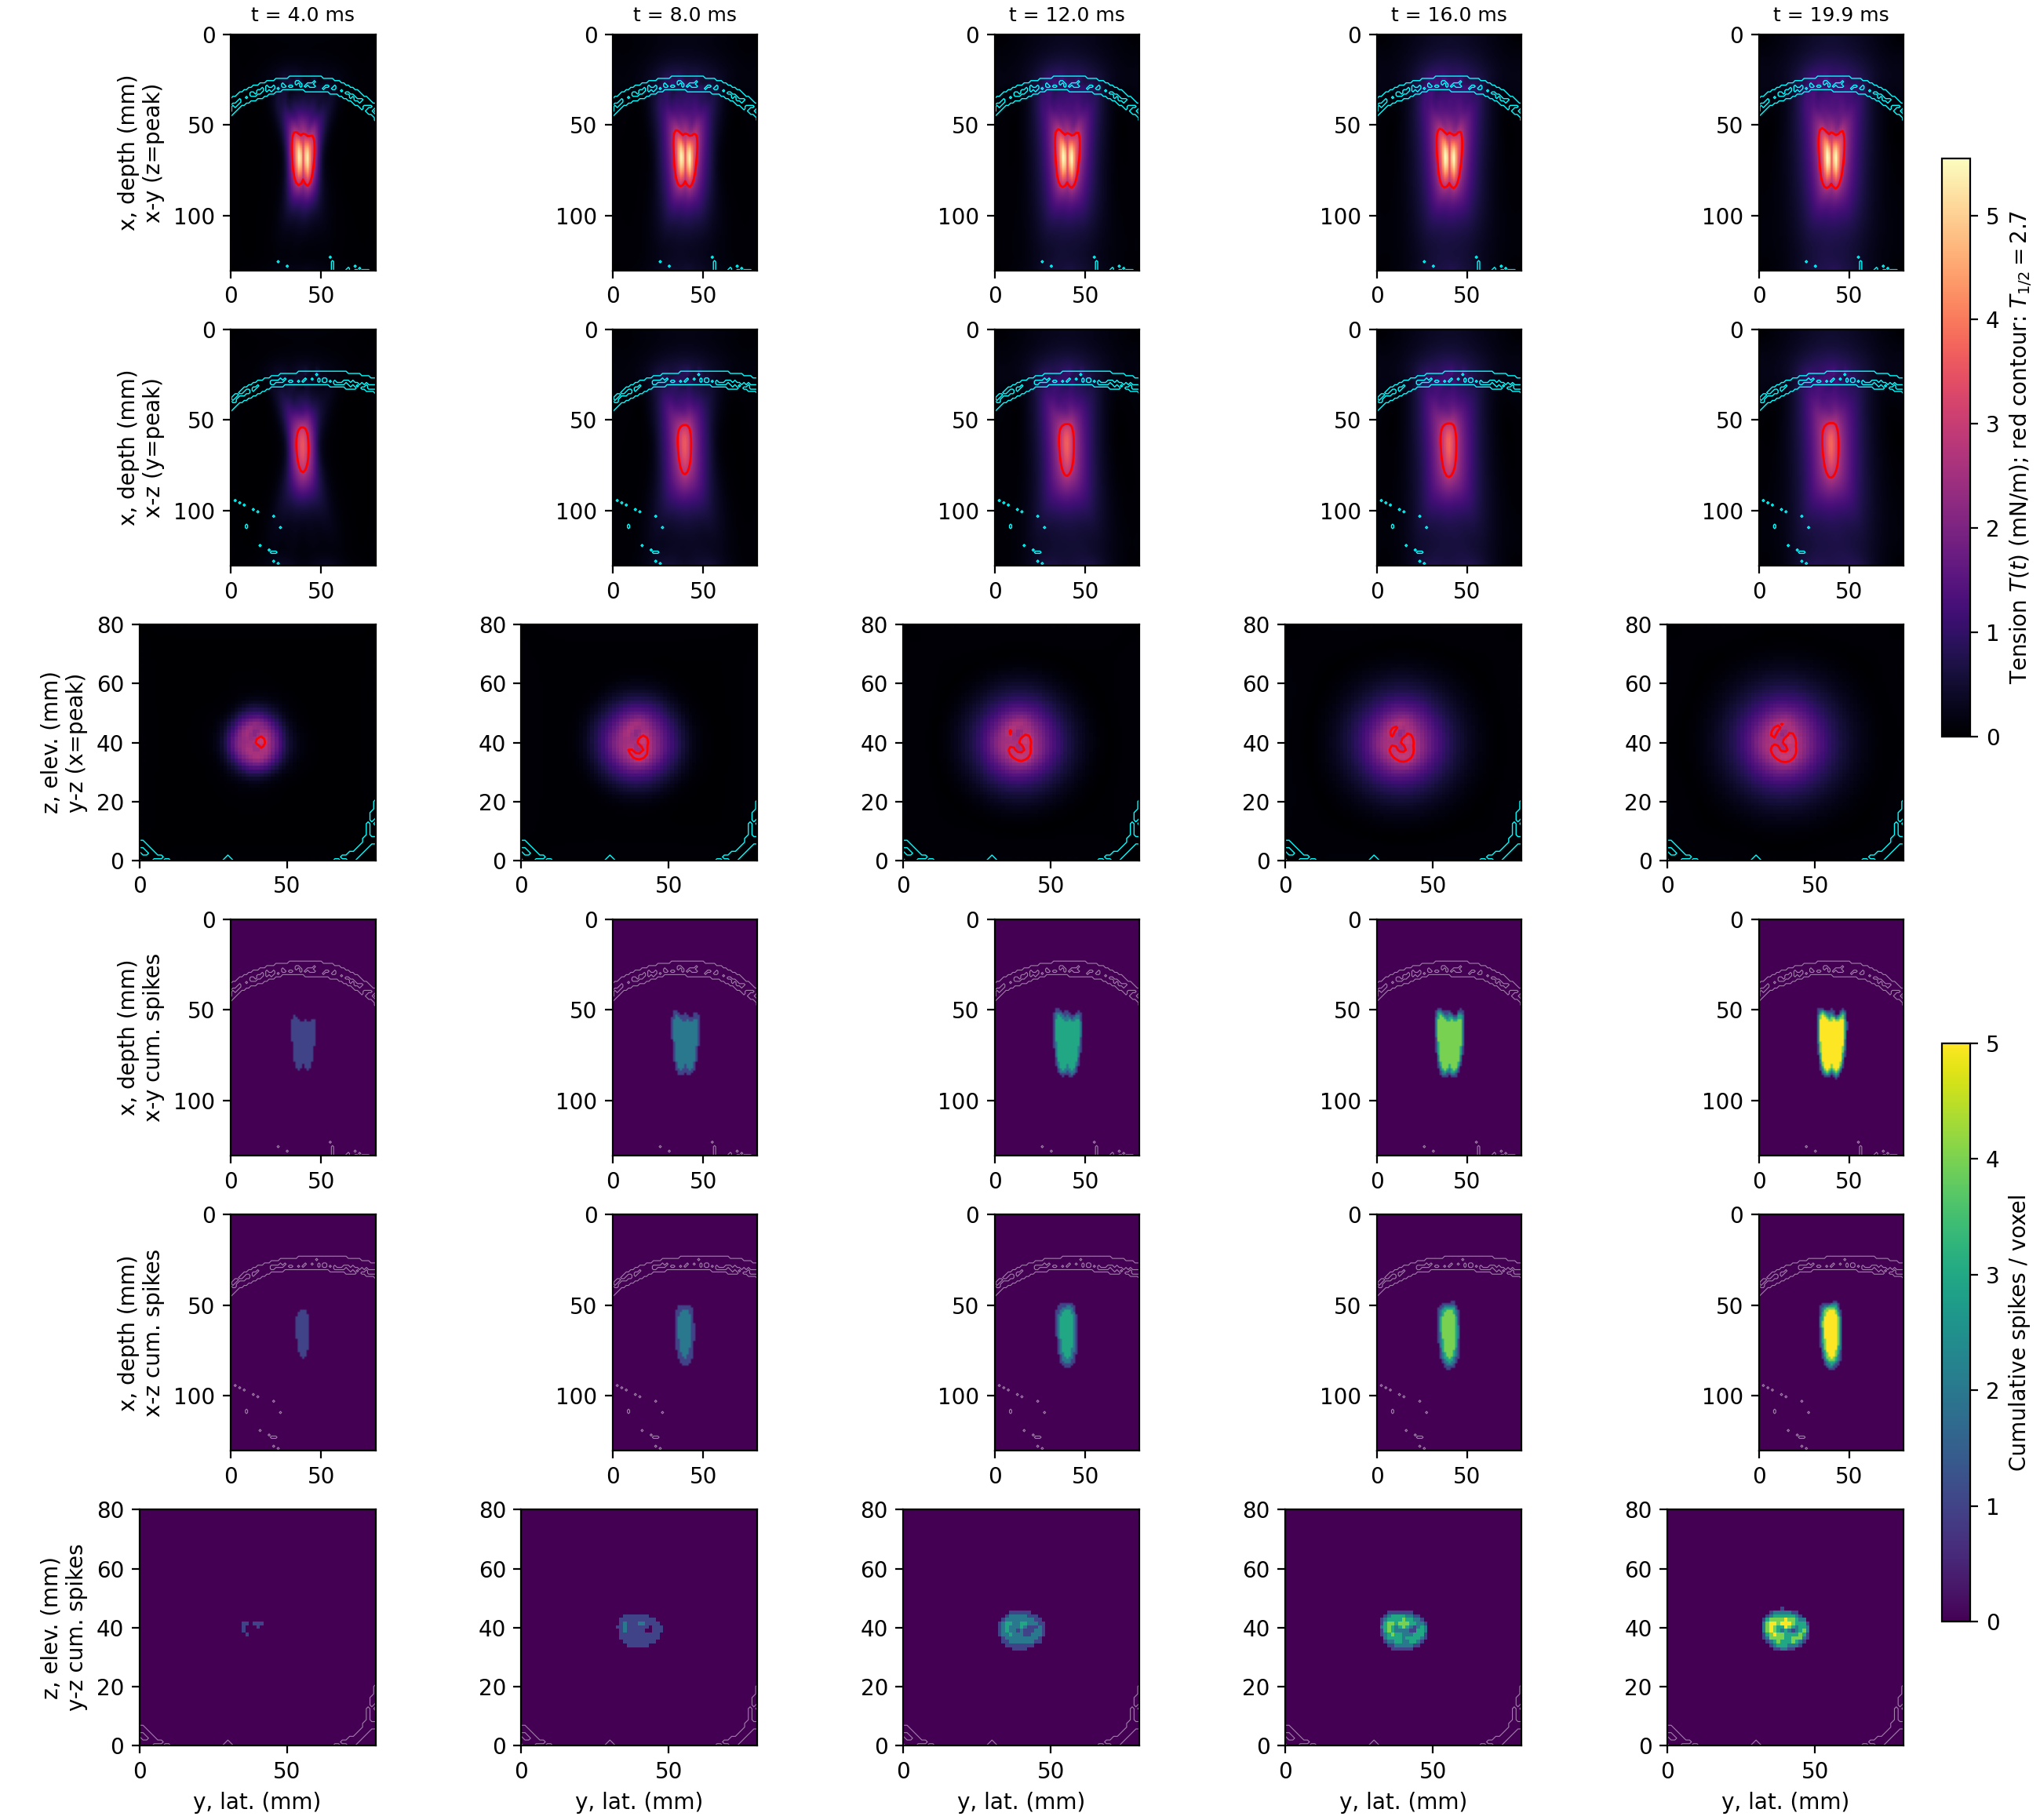
\includegraphics[width=\linewidth]{neural_snapshot_row.png}
\caption{Top row: instantaneous tension on the focal y-z slice at five within-burst times.  Bottom row: cumulative spike count per voxel up to the same time.  The pair makes the mechano $\to$ spike lag visible: voxels recruit a few ms after their tension crests.}\label{fig:neural_snapshots}
\end{figure}

\subsection{Spike raster with anatomical key}\label{sec:neural_raster}
\begin{figure}[H]\centering
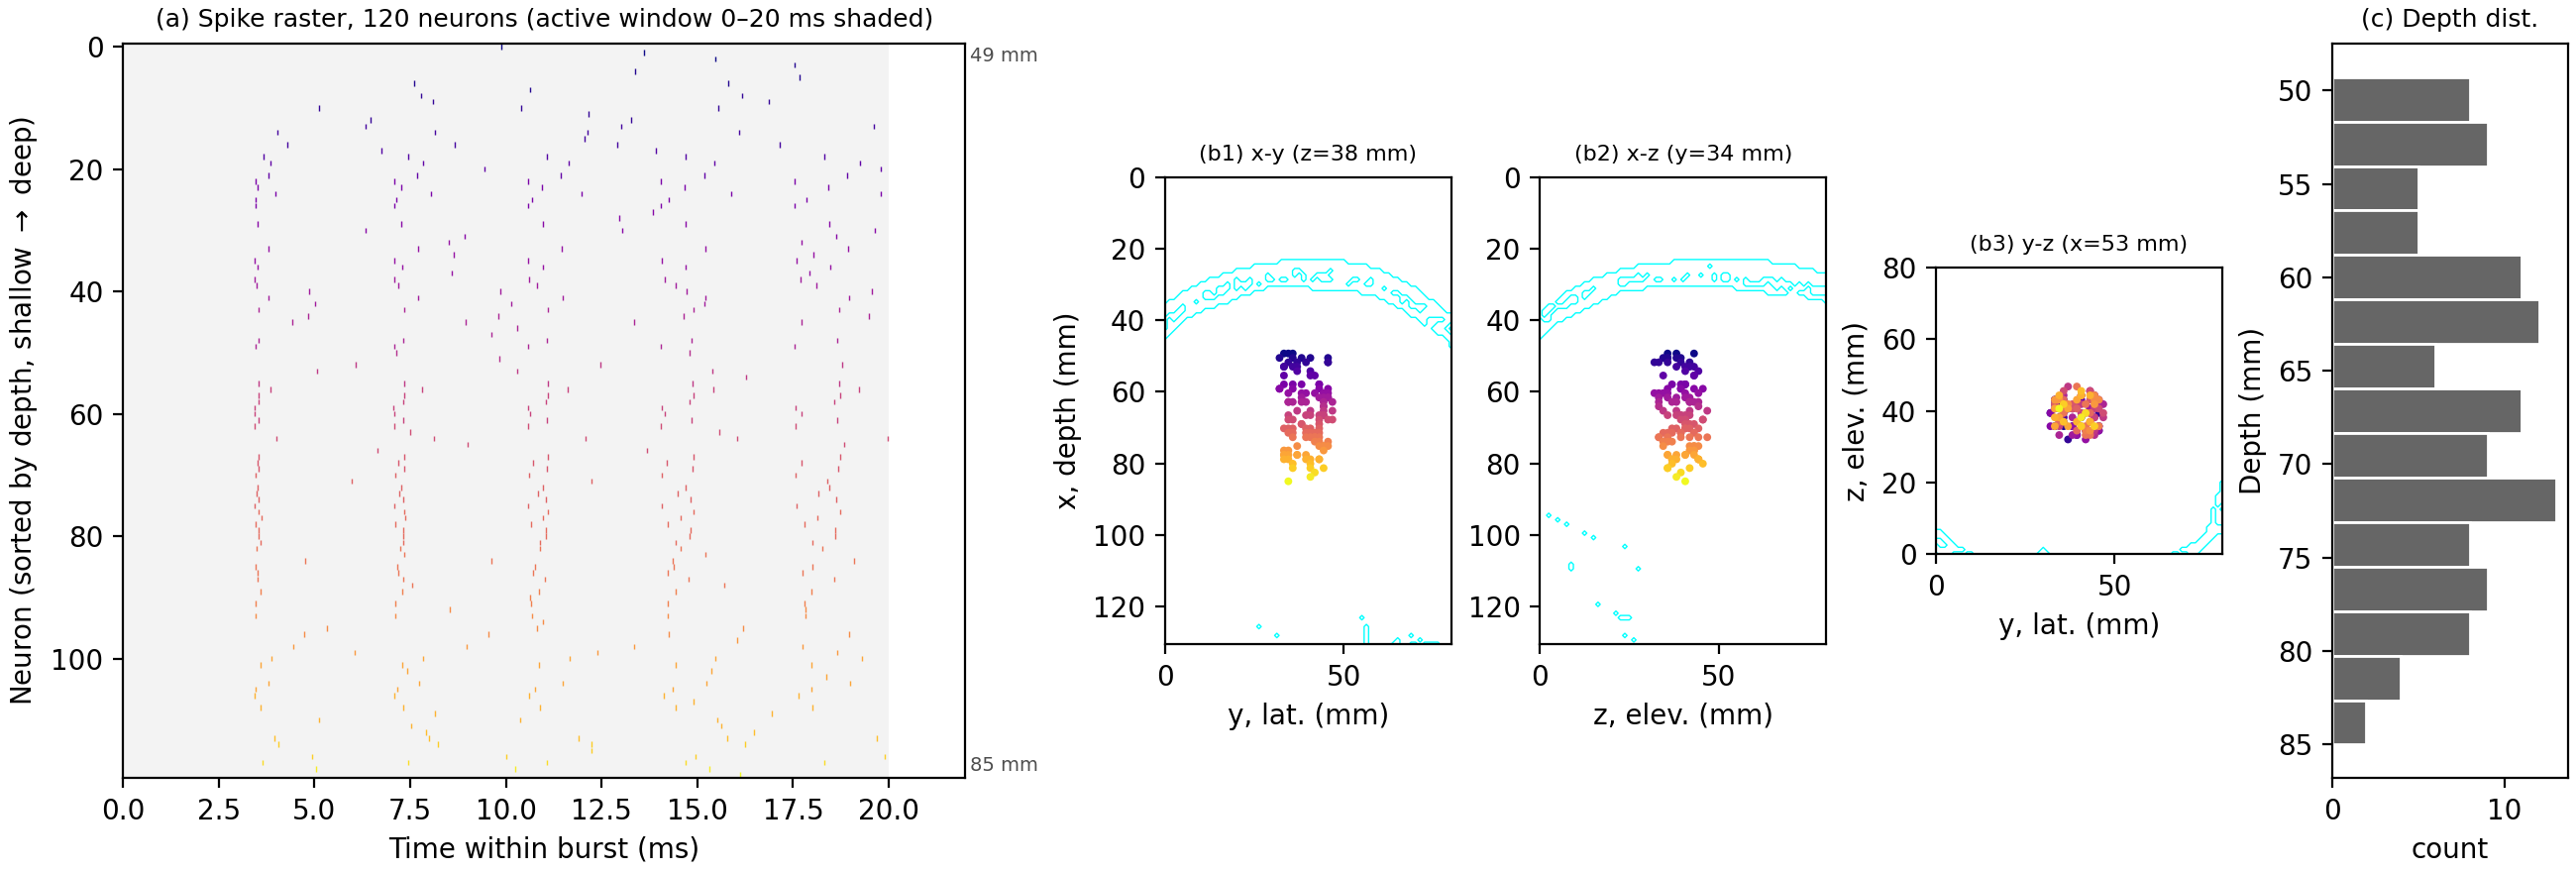
\includegraphics[width=\linewidth]{neural_raster.png}
\caption{(a) Per-burst spike raster sampled across firing voxels, sorted by depth and replicated across three theta groups; tick colour encodes depth.  (b) The same neurons drawn on the focal y-z slice, coloured by depth --- links each raster row back to anatomy.  (c) Depth distribution of the sample.}\label{fig:neural_raster}
\end{figure}

\subsection{Population PSTH and recruitment}\label{sec:neural_psth}
\begin{figure}[H]\centering
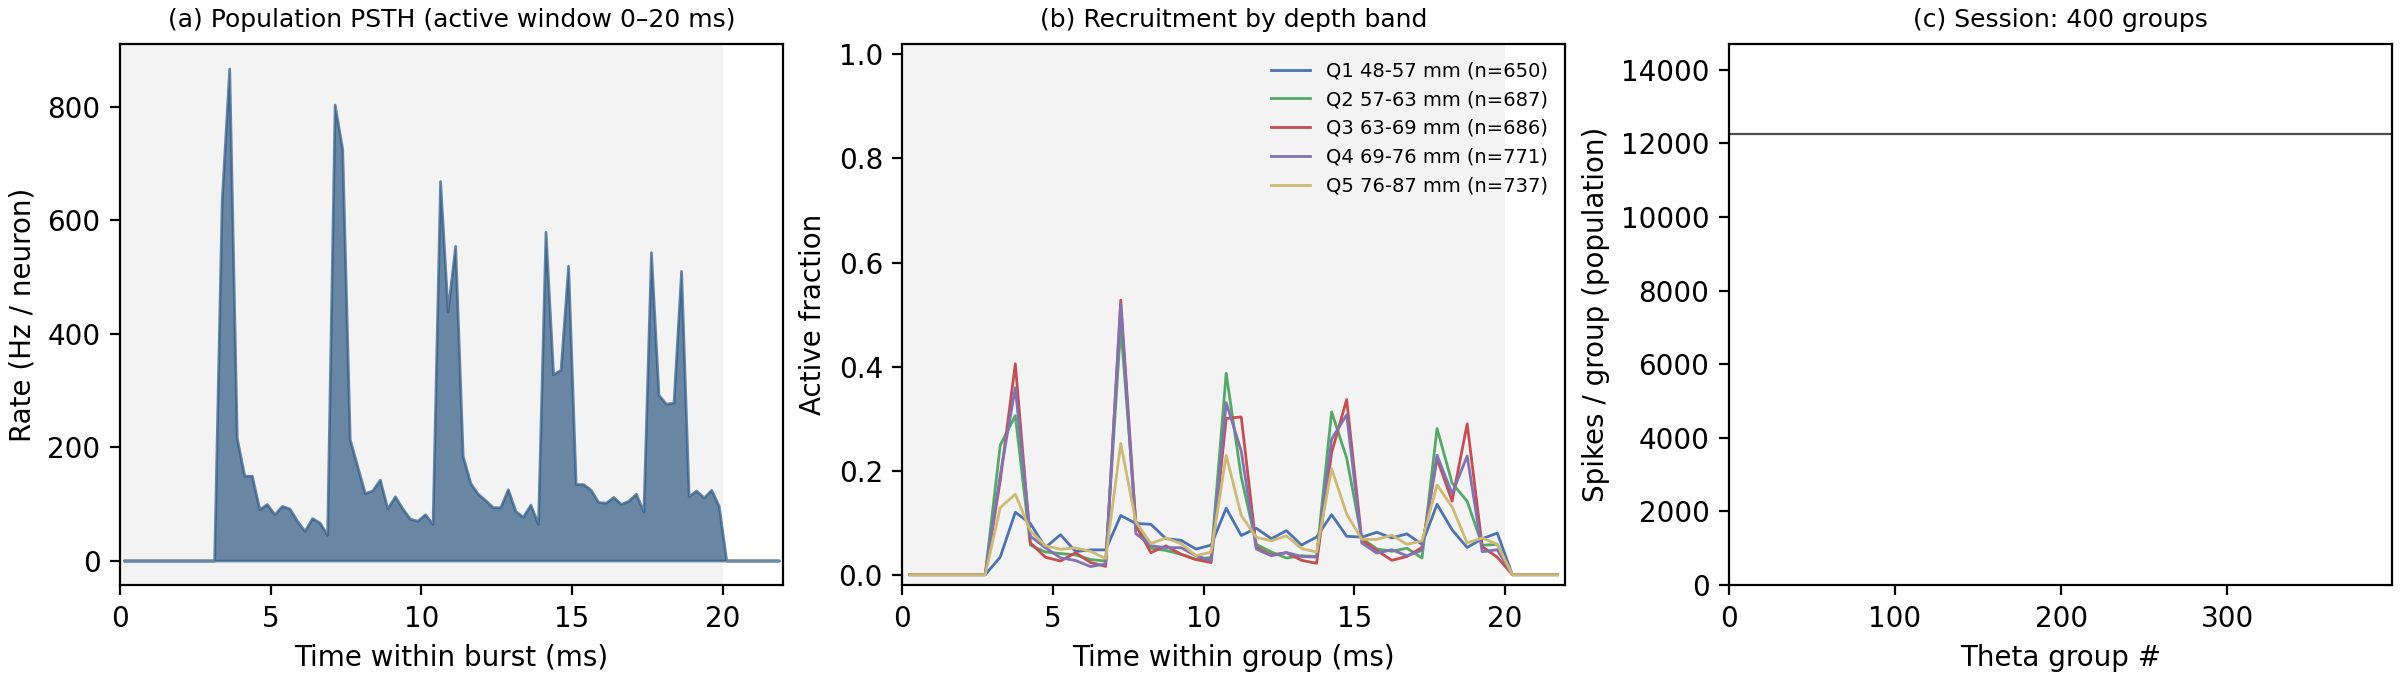
\includegraphics[width=\linewidth]{neural_psth.png}
\caption{(a) Population-mean PSTH over one theta-group period.  (b) Active-fraction recruitment split by depth band (shallow / mid / deep relative to focus).  (c) Per-group spike total over the 400-group session schedule.}\label{fig:neural_psth}
\end{figure}

\subsection{Rate distribution and spectral content}\label{sec:neural_distrib}
\begin{figure}[H]\centering
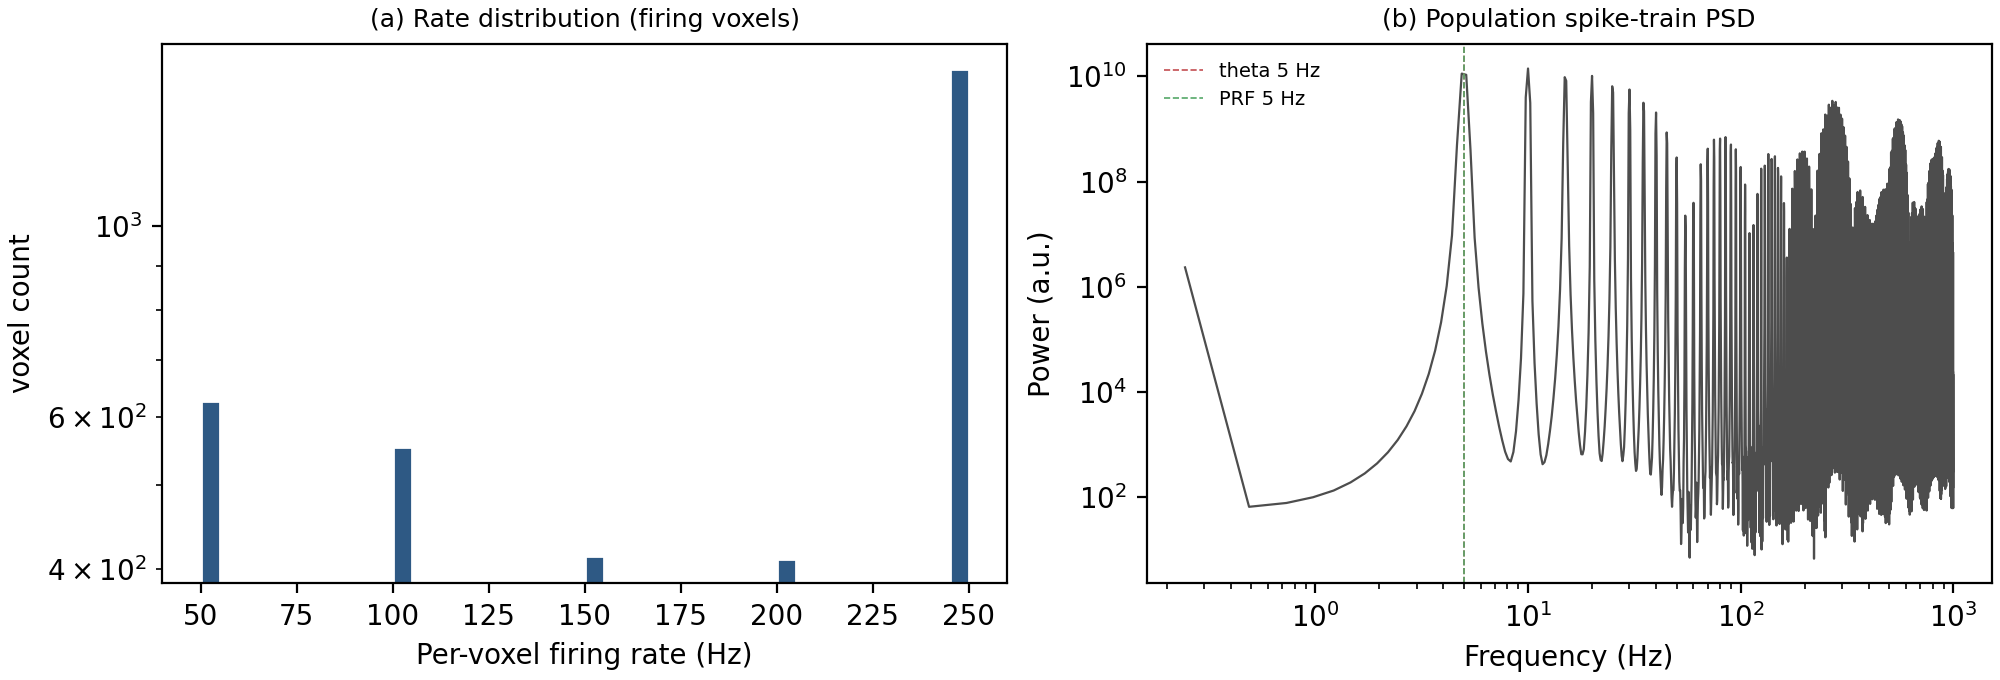
\includegraphics[width=\linewidth]{neural_distrib.png}
\caption{(a) Per-voxel firing-rate distribution across firing voxels (log $y$).  (b) Population spike-train PSD, log--log; vertical guides at the within-burst PRF and the theta envelope frequency test whether the simulated response carries the protocol's nominal rhythms.}\label{fig:neural_distrib}
\end{figure}

\subsection{Firing volume vs.\ time}\label{sec:neural_volume_t}
\begin{figure}[H]\centering
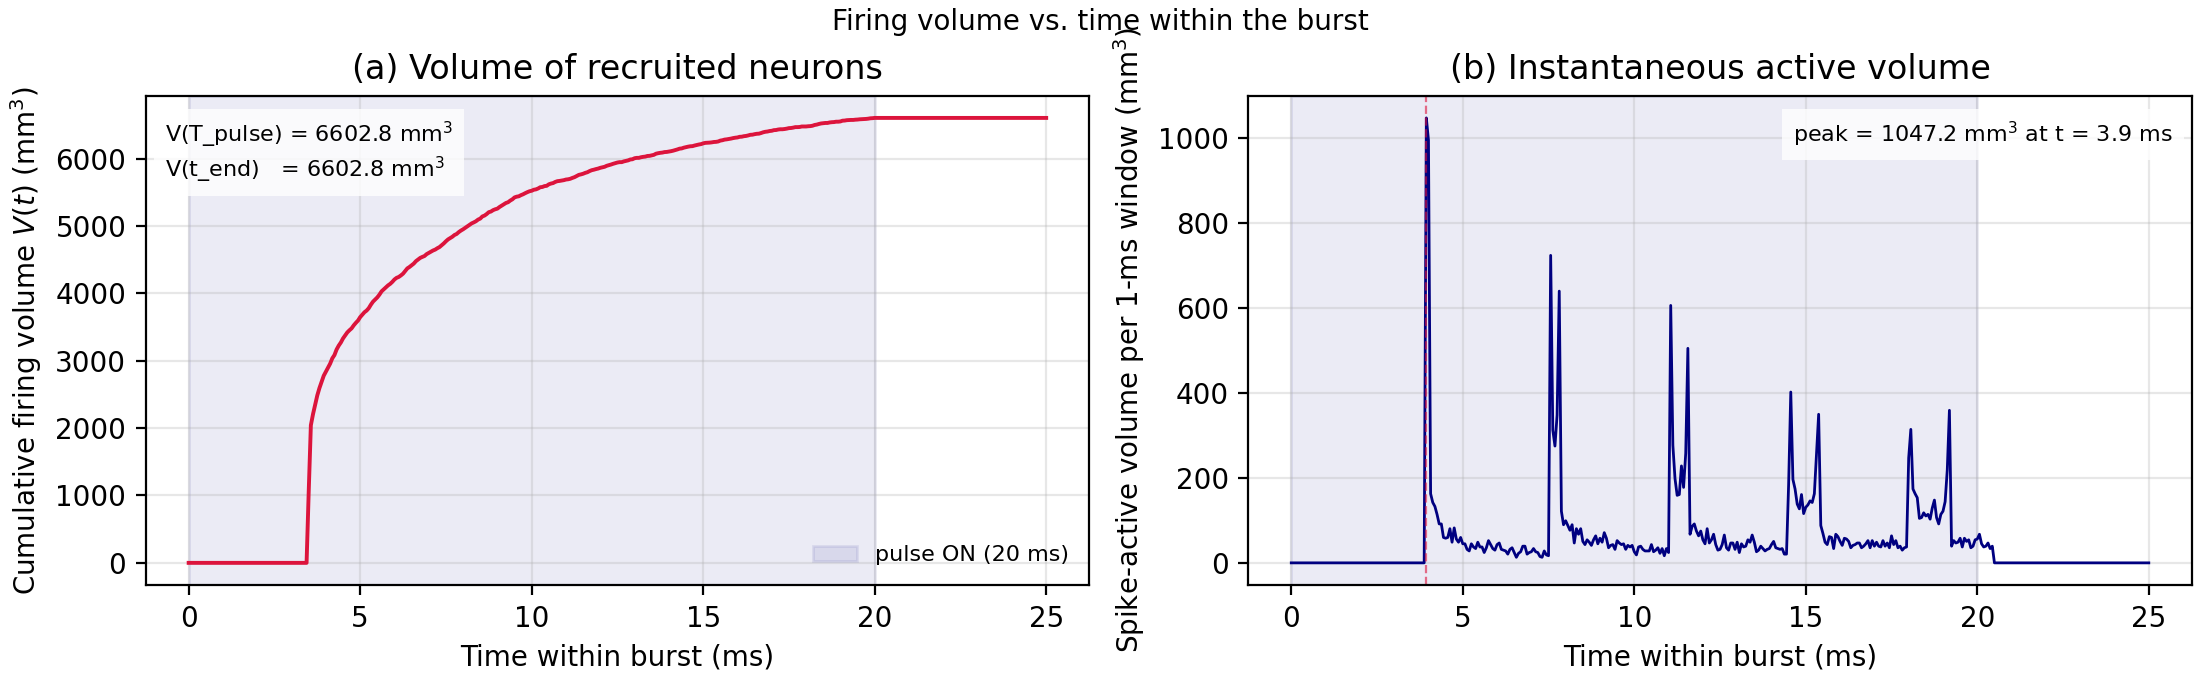
\includegraphics[width=\linewidth]{neural_volume_t.png}
\caption{Volumetric recruitment within the burst.  (a) Cumulative volume of brain that has fired at least one spike by time $t$; the navy band marks the pulse-on window.  (b) Spike-active volume in a rolling 1\,ms window --- the volumetric analogue of a population PSTH.  Volumes use the FDTD voxel pitch ($\sim 1.87$~mm$^3$ / voxel).  Cumulative volume at pulse end: 6602.8~mm$^3$; peak instantaneous active volume: 1047.2~mm$^3$.}\label{fig:neural_volume_t}
\end{figure}

\subsection{Mechanosensitive gating curves}\label{sec:neural_gating}
\begin{figure}[H]\centering
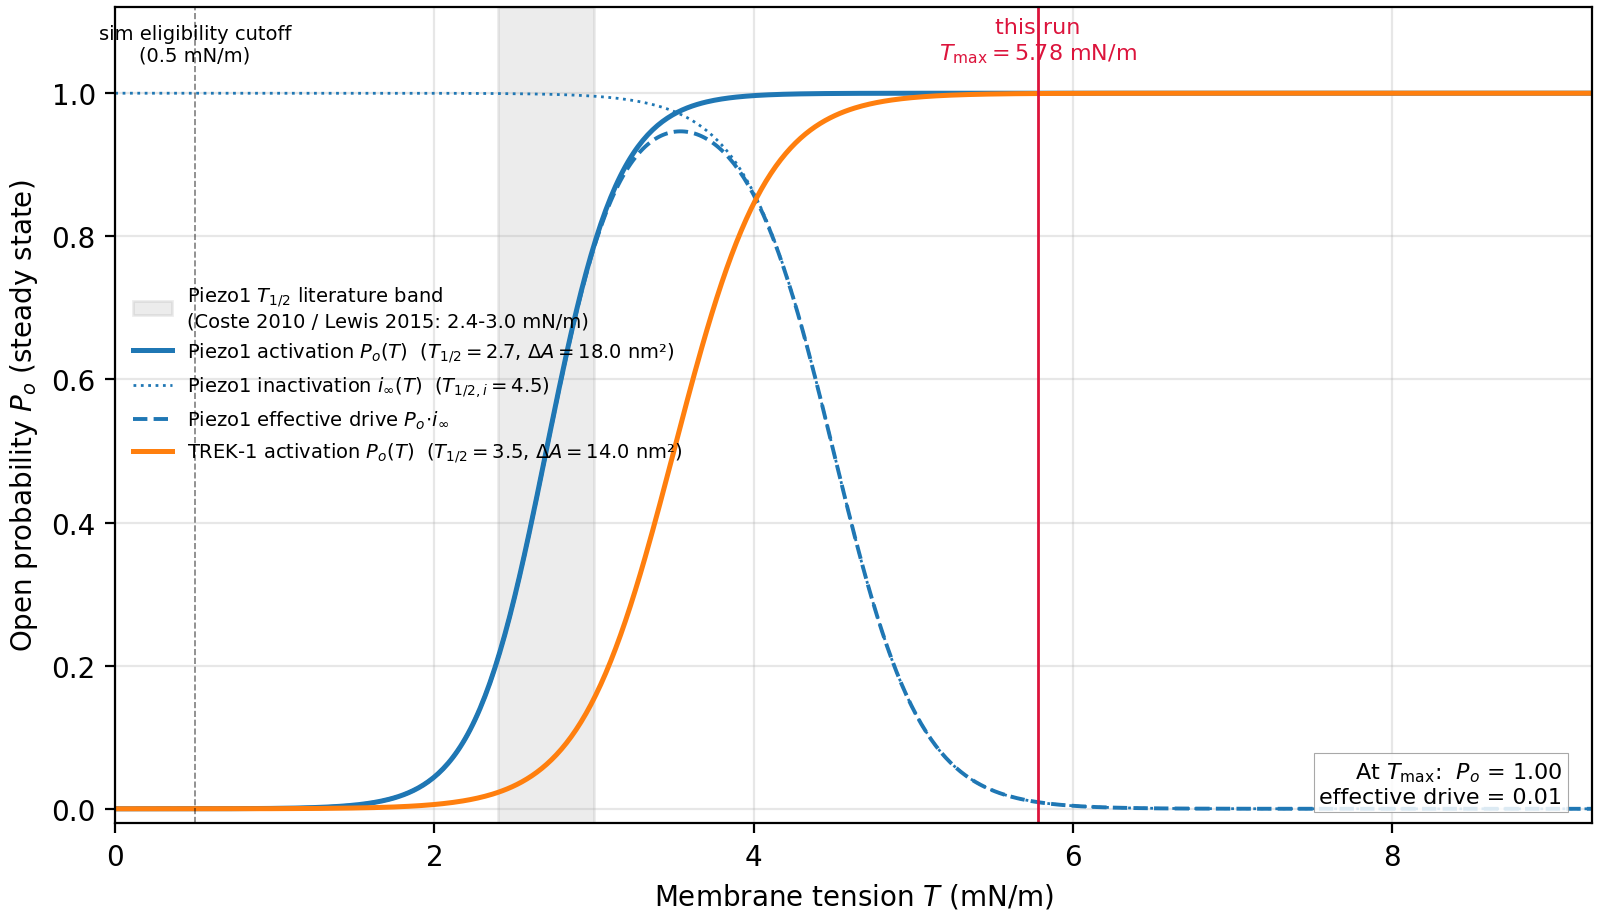
\includegraphics[width=0.92\linewidth]{neural_gating.png}
\caption{Boltzmann gating curves used for the strain-driven channels in this sim, overlaid with literature anchors and the per-sim working point.  Solid: activation $P_o(T)$; dotted (Piezo1 only): inactivation $i_\infty(T)$; dashed: effective drive $P_o \cdot i_\infty$.  Grey band: literature confidence interval on the Piezo1 half-activation $T_{1/2}$ (Coste 2010 / Lewis 2015: 2.4--3.0~mN/m).  Crimson vertical: peak tension reached in this sim.  Black dashed: tension-threshold cutoff used by the eligibility filter in \texttt{run\_neural\_sim.py}.}\label{fig:neural_gating}
\end{figure}

\subsection{Representative cells}\label{sec:neural_representative}
\begin{figure}[H]\centering
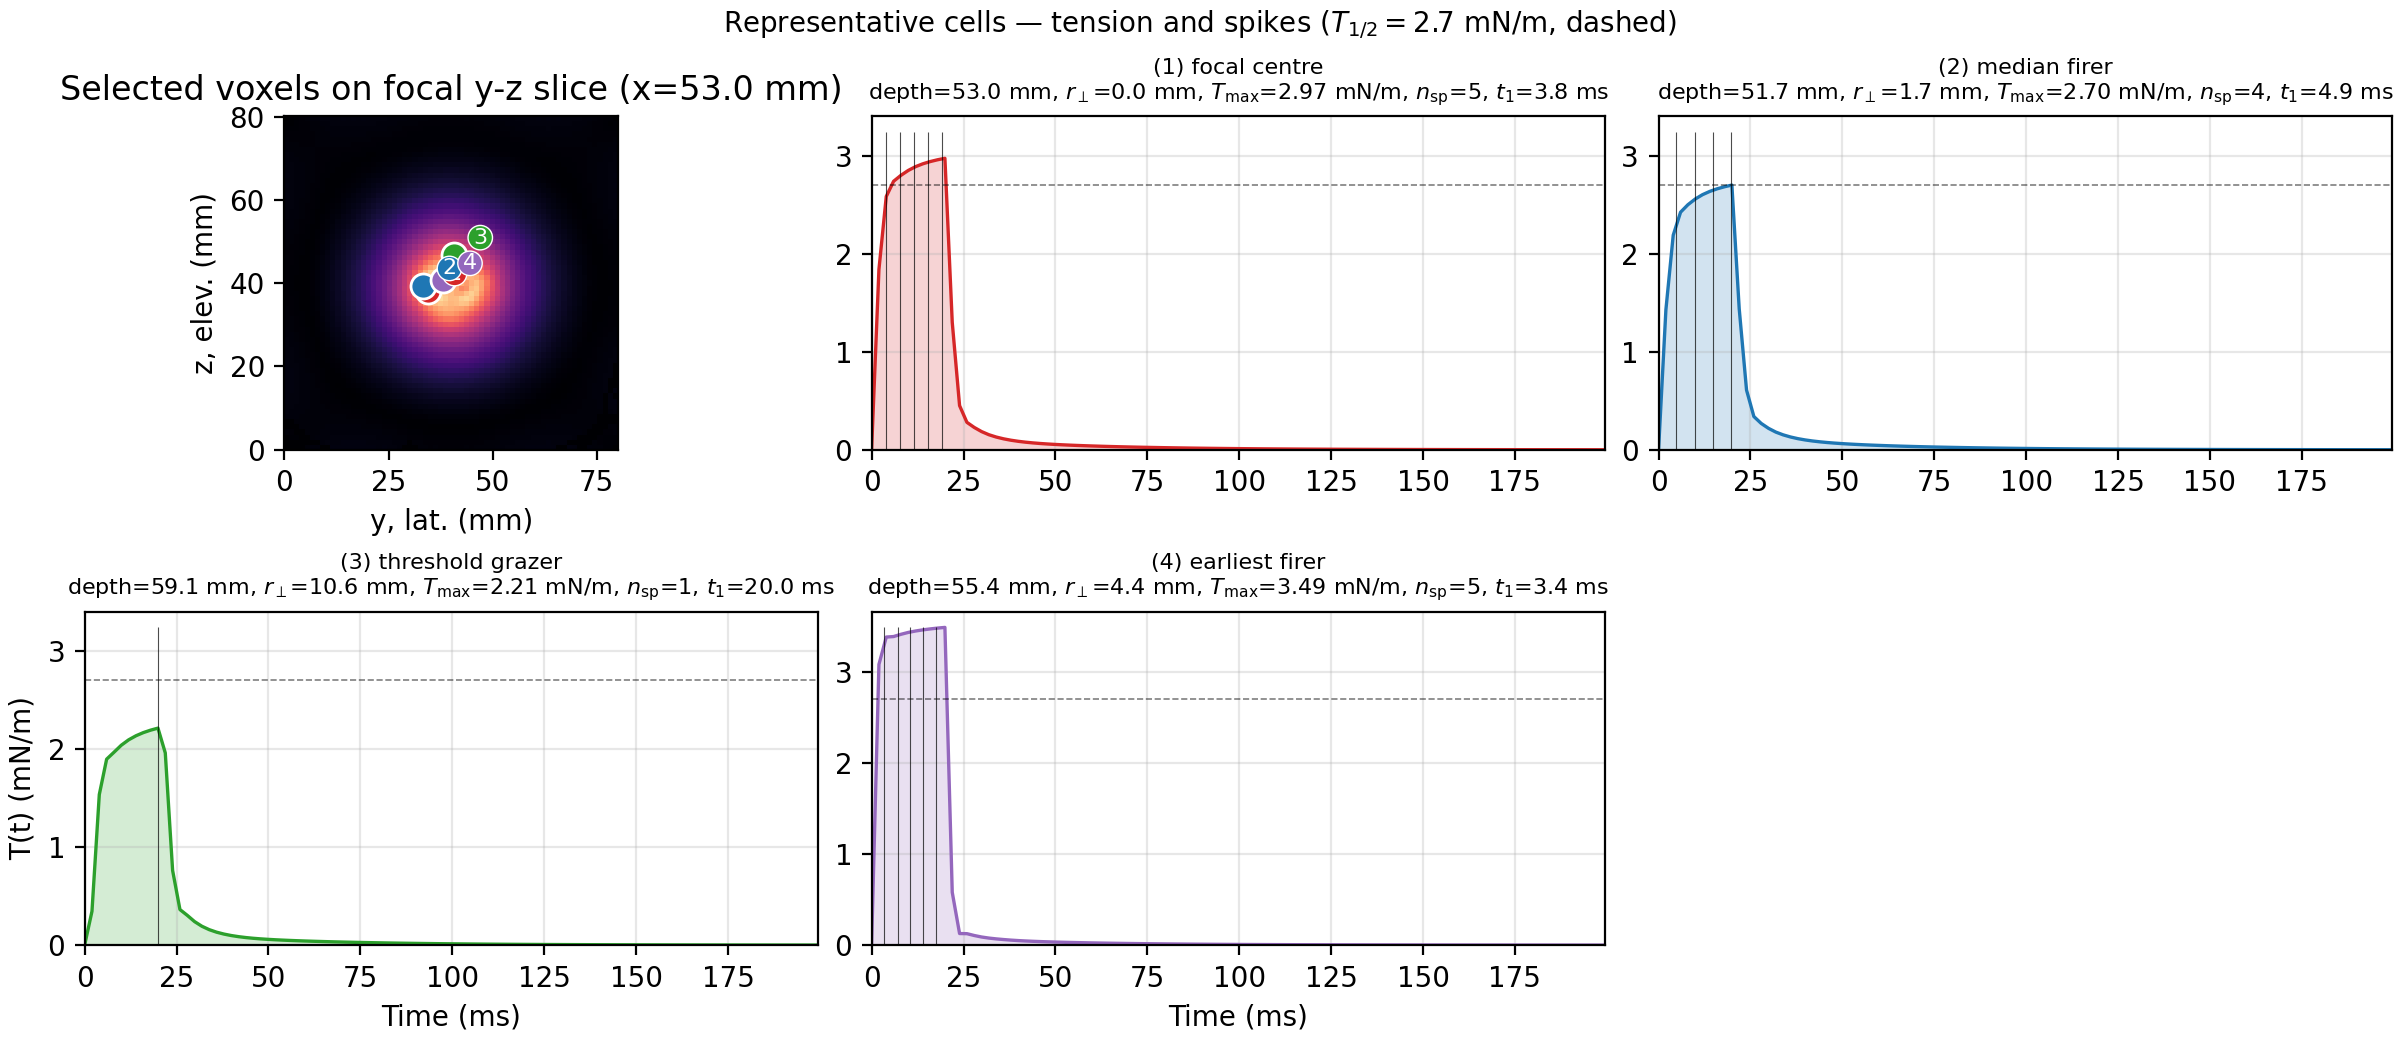
\includegraphics[width=\linewidth]{neural_representative.png}
\caption{Five voxels selected to span the firing-zone phenomenology: focal centre (highest peak tension); median firer (median spike count); threshold grazer (lowest peak tension that still fires); earliest firer (smallest first-spike latency); latest firer (largest first-spike latency).  Top-left: positions on the focal y-z slice, overlaid on the peak-tension field.  Trace panels: per-voxel membrane-tension trajectory $T(t)$ from the saved displacement-4D field, with the Piezo1 half-activation $T_{1/2} = 2.7$~mN/m drawn as a dashed line and the recorded spike times overlaid as black vlines.  Annotation box reports depth, lateral distance from focus $r_\perp$, peak tension, spike count, and first-spike latency for each cell.}\label{fig:neural_representative}
\end{figure}







\section{Astrocytic TRPA1 relay (non-Piezo mechanism)}\label{sec:astrocyte_outputs}

The astrocytic ultrasound-neuromodulation pathway of Oh et al.\ 2019 is
scored on the same per-voxel peak-tension field: ultrasound gates
mechanosensitive TRPA1 in astrocytes ($T_{1/2} = 6.0$~mN/m),
the resulting Ca\textsuperscript{2+} influx charges a slow astrocytic pool
($\tau_{\mathrm{Ca}} = 300$~ms), Ca\textsuperscript{2+}-triggered
glutamate release drives neuronal NMDA receptors, and the NMDA current
depolarises the neuron.  Unlike the per-pulse channel mechanisms, the
relay accumulates over the sonication, so its drive grows with duty
cycle $\times$ on-time rather than tracking the carrier.

\begin{table}[H]\centering\footnotesize
\caption{Astrocytic-NMDA relay metrics at the focal voxel and protocol duty / session on-time.}
\begin{tabular}{l r l}
\toprule
\textbf{Quantity} & \textbf{Value} & \textbf{Unit} \\
\midrule
Focal peak tension                 & 5.78   & mN/m \\
Peak astrocytic-NMDA drive         & 0.012          & 0--1 \\
Recruited voxels (drive $>$ 0.05)  & 0 & voxels \\
Focal depolarisation (500 ms)      & 7.5 & mV \\
Focal spikes (500 ms)              & 0                       & -- \\
Duty cycle / session               & 0.10 / 80 & -- / s \\
\bottomrule
\end{tabular}
\end{table}

\begin{figure}[H]\centering
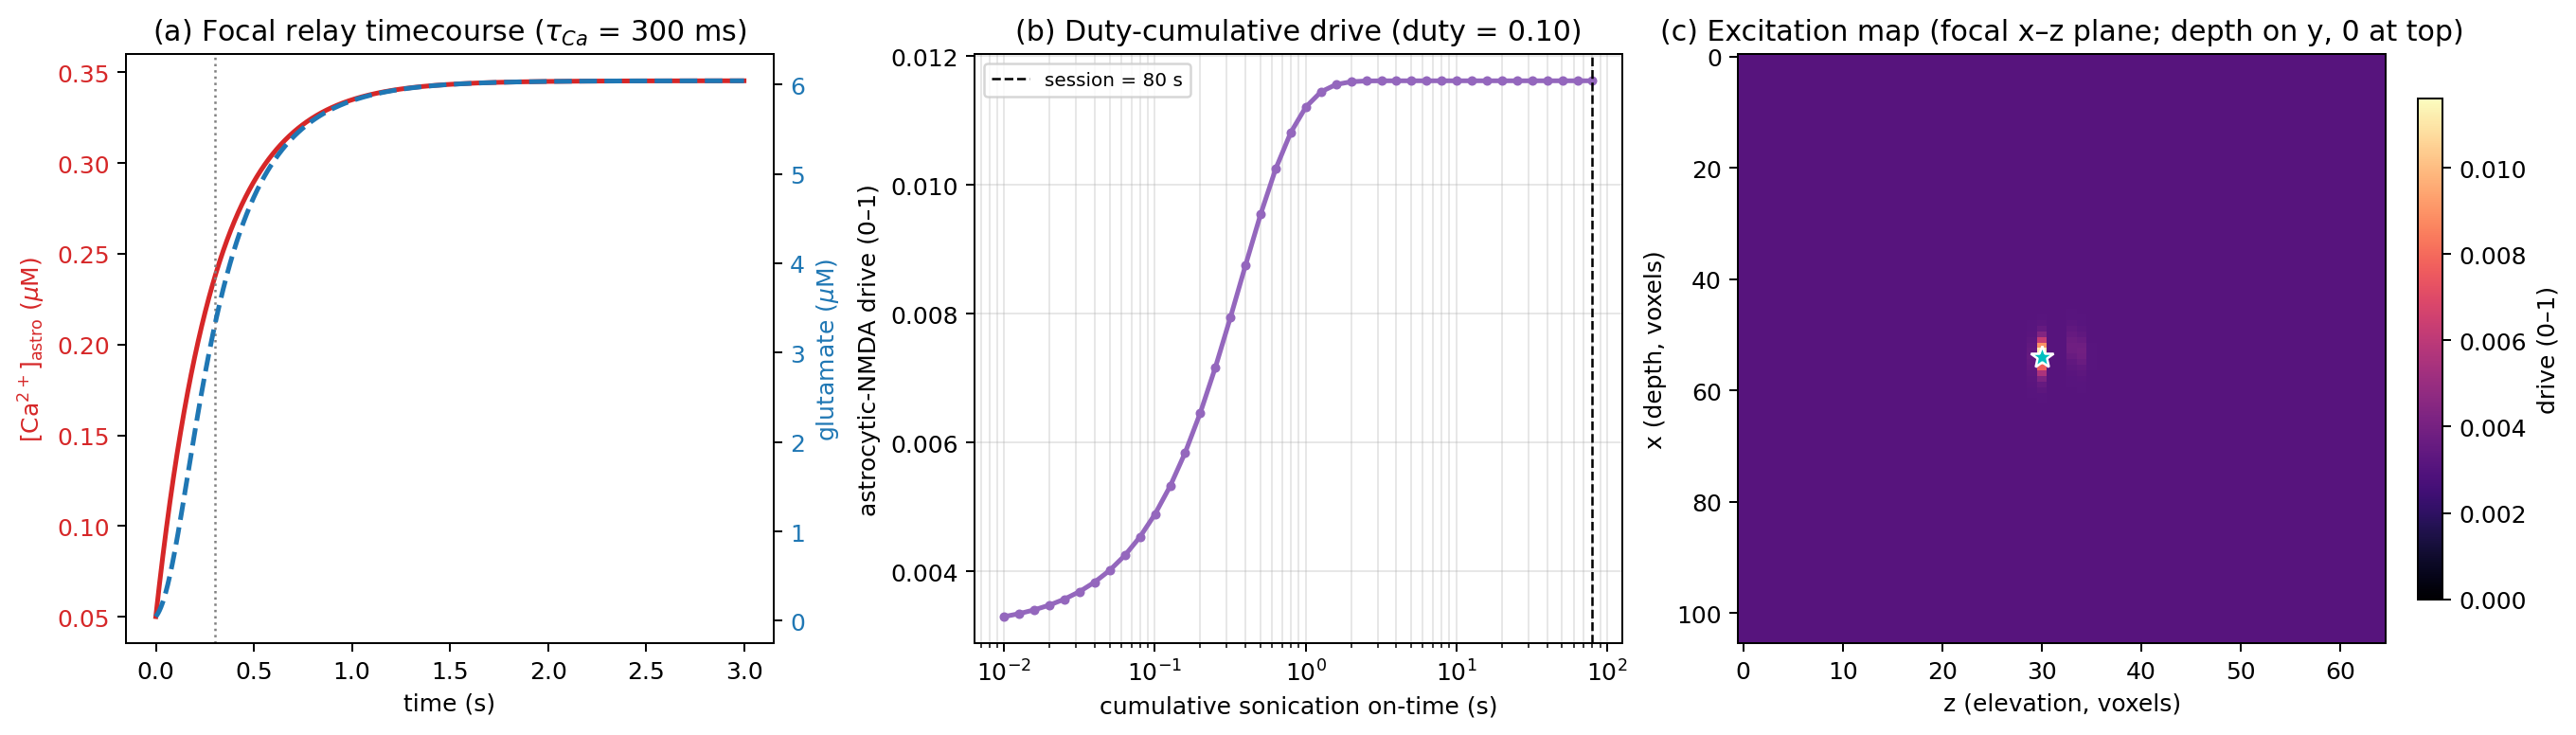
\includegraphics[width=\linewidth]{astrocyte_pathway.png}
\caption{Astrocytic TRPA1 $\to$ Ca\textsuperscript{2+} $\to$ glutamate $\to$ NMDA relay on the canonical field.  (a)~Focal-voxel relay timecourse: the slow astrocytic Ca\textsuperscript{2+} (red) and glutamate (blue dashed) rise over hundreds of ms, the defining slowness of the pathway.  (b)~Astrocytic-NMDA excitation drive versus cumulative sonication on-time --- the duty-cumulative signature that distinguishes this pathway from the per-pulse channel mechanisms; the dashed line marks the protocol session duration.  (c)~Per-voxel astrocytic-NMDA excitation map on the focal $x$--$z$ plane (cyan star: focal voxel).}\label{fig:astrocyte_pathway}
\end{figure}




\section{Mechanosensitive synaptic and voltage-gated transmission (sixth mechanism)}\label{sec:synaptic_outputs}

The sixth candidate mechanism scores mechanosensitive \emph{synaptic} and
\emph{voltage-gated} transmission on the same per-voxel peak-tension field.
It bundles three literature-grounded effects, each exposing a closed-form
per-case scalar gain: presynaptic vesicle-release modulation
$P_r(T)/P_r(0)$ (Tyler 2018), post-synaptic NMDA stretch enhancement
$f_{\mathrm{stretch}}(T)$ (Maneshi et al.\ 2017), and a hyperpolarising
shift of the voltage-gated Na\textsuperscript{+}/Ca\textsuperscript{2+}
activation that raises the Na\textsuperscript{+} current
($k_{\mathrm{mechano}} = 0.30$~mV per
mN/m; Kubanek et al.\ 2016).  Unlike the astrocytic relay these effects act
on the fast (per-pulse) synaptic and spike-generating machinery; their
product is a single multiplicative excitation gain that drives a
post-synaptic Hodgkin--Huxley neuron through an AMPA/NMDA synapse.

\begin{table}[H]\centering\footnotesize
\caption{Synaptic / voltage-gated (M6) metrics at the focal voxel.}
\begin{tabular}{l r l}
\toprule
\textbf{Quantity} & \textbf{Value} & \textbf{Unit} \\
\midrule
Focal peak tension                 & 5.78    & mN/m \\
Peak combined pathway gain         & 9.68   & $\times$ \\
Recruited voxels (gain $>$ 1.5)  & 17143 & voxels \\
Focal depolarisation (120 ms)      & 116.1 & mV \\
Focal spikes (120 ms)              & 10                        & -- \\
$P_r$ range / $\alpha_{\mathrm{NMDA}}$ & 0.10--0.60 / 1.0 & -- \\
\bottomrule
\end{tabular}
\end{table}

\begin{figure}[H]\centering
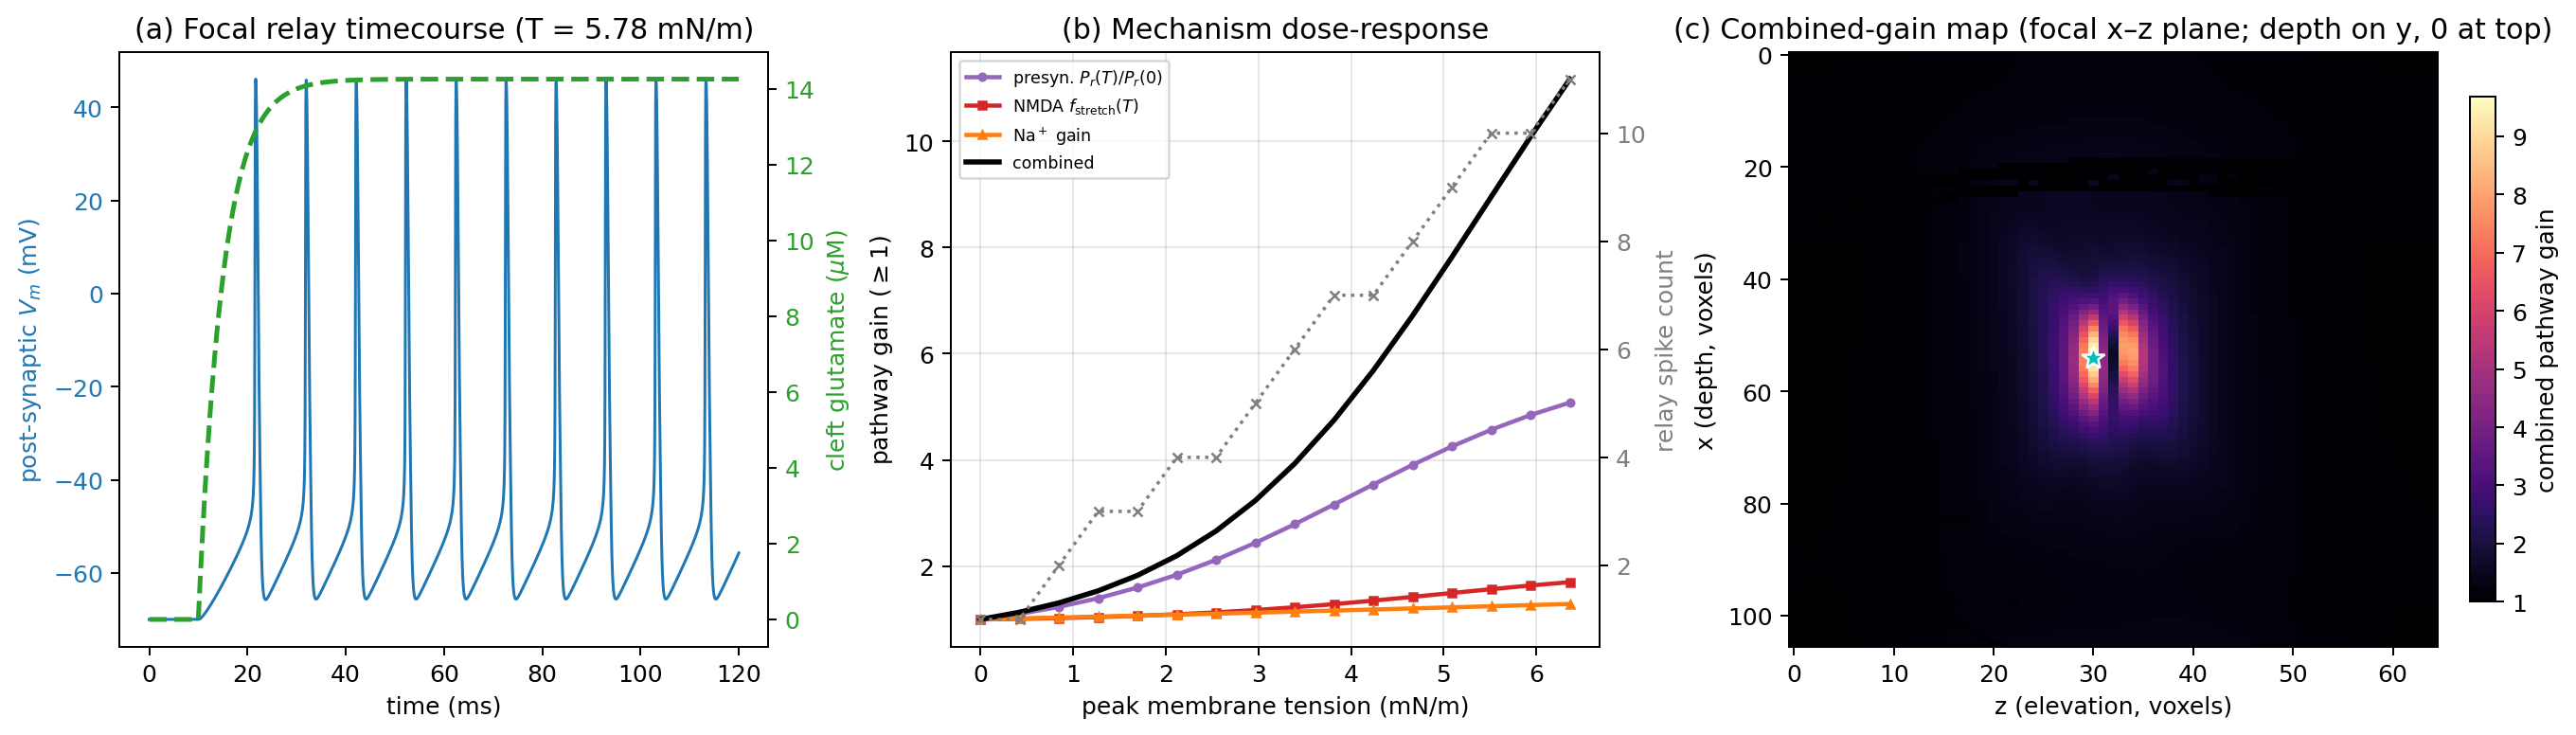
\includegraphics[width=\linewidth]{synaptic_pathway.png}
\caption{Mechanosensitive synaptic and voltage-gated transmission on the canonical field.  (a)~Focal-voxel relay timecourse: presynaptic tension-modulated release drives a cleft glutamate transient (green dashed) and post-synaptic firing (blue).  (b)~Mechanism dose-response: the three closed-form scalar gains --- presynaptic $P_r(T)/P_r(0)$, NMDA $f_{\mathrm{stretch}}(T)$, and Na\textsuperscript{+} current gain --- with their product (black), and the relay spike count (grey dotted, right axis) versus peak tension.  (c)~Per-voxel combined pathway-gain map on the focal $x$--$z$ plane (cyan star: focal voxel).}\label{fig:synaptic_pathway}
\end{figure}


\end{document}
